% This work is licensed under the Creative Commons Attribution-Share Alike 2.0 France License.
% To view a copy of this license, visit http://creativecommons.org/licenses/by-sa/2.0/fr/legalcode
% or send a letter to Creative Commons, 171 Second Street, Suite 300, San Francisco, California, 94105, USA.
\documentclass[12pt,french]{book}
	%\documentclass[a4paper,12pt,french]{book}
\usepackage{xunicode}
\usepackage{fontspec}
\usepackage{xltxtra}
\usepackage[francais]{babel} 
\usepackage{xspace}
\defaultfontfeatures{Mapping=tex-text}
\usepackage[a4paper, margin=2cm]{geometry}
	%\usepackage[paperwidth=150mm, paperheight=200mm, margin=2cm]{geometry}
\usepackage{xelibertine}
\setmainfont{Linux Libertine O}
\usepackage{listings}
\usepackage{color}
\usepackage{fix-cm}
\usepackage{fancybox}
\usepackage{eurosym}
\usepackage{makeidx} 
\usepackage[Bjornstrup]{fncychap}
\usepackage[xetex=true, colorlinks=true, linkcolor=blue, urlcolor=blue]{hyperref}
\usepackage{scalefnt}
\usepackage{fancyvrb}
\usepackage{float}
\usepackage{subfigure}
\usepackage[all]{hypcap}
\usepackage[tight]{shorttoc}
\newcommand{\sommaire}{\shorttoc{Sommaire}{0}}
%\newfontfamily\zhfont[BoldFont=AR PL New Sung]{AR PL New Sung}
\hypersetup{ % Modifiez la valeur des champs suivants
	    pdfauthor   = {Jason R. Briggs \& Michel Weinachter},%
	    pdftitle    = {Domptage de serpent pour les enfants},%
	    pdfsubject  = {Apprendre à programmer avec Python},%
	    pdfkeywords = {Python programmation débutant enfant},%
	    pdfcreator  = {XeTeX},%
	    pdfproducer = {XeTeX}%
	    }
\usepackage{eso-pic}
\newcommand\BackgroundPicture{
	 \put(0,0){
	 \parbox[b][\paperheight]{\paperwidth}{
	 \vfill
	 \centering
	 
\includegraphics[width=5cm]{images/python.pdf}
	 \vfill
	 }}} 
\setromanfont[Mapping=tex-text]{Linux Libertine O}
\setsansfont[Mapping=tex-text]{Linux Biolinum O}
\renewcommand{\chaptermark}[1]{\markboth{ #1}{}}
\renewcommand{\sectionmark}[1]{\markright{ #1}{}}
\title{Domptage de serpent pour les enfants}
\author{Jason R. Briggs \& Michel Weinachter}
\date{17 février 2009}
\definecolor{bleu}{rgb}{0,0,0.4}
\definecolor{lbleu}{rgb}{0.9,0.9,1}
\definecolor{mbleu}{rgb}{0.5,0.5,1}
\definecolor{gray}{rgb}{0.7,0.7,0.7}
%\makeindex
\newcommand{\clearemptydoublepage}{%
	\newpage{\pagestyle{empty}\cleardoublepage}}
%\documentclass[12pt,leqno,a4paper]{book}
%\usepackage[dvips]{graphicx}
%\usepackage[usenames]{color}
%\usepackage[colorlinks,pdfauthor={Jason R Briggs},pdftitle={Snake Wrangling for Kids - Learning to Program with Python},pdfsubject={Programming for Kids},pdfkeywords={python,kids,programming}]{hyperref}
%\usepackage{longdiv}
%\usepackage{makeidx}
\usepackage{versions}

\excludeversion{WINDOWS}

\includeversion{LINUX}

\excludeversion{MAC}

%\usepackage[absolute]{textpos}
%\usepackage{wrapfig}
%\usepackage{eso-pic}
	%\usepackage{nameref}
	%\usepackage{backref}
	%\usepackage{appendix}
	%\usepackage{upquote}
	%\usepackage[math-style=tex]{unicode-math} 
	%\usepackage{hyperref}
	%\usepackage[toc]{appendix}
	%\usepackage{memoir}
	%\usepackage{geometry}
	%\usepackage{zhspacing}
	%\zhspacing
	%\geometry{%
	%a4paper
	%paperwidth=140mm, paperheight=225mm
	%}
	%\usepackage{cleverref}
	%\usepackage{varioref}
	%\setlength{\overfullrule}{1cm}
	%
	%\newcommand\TitlePicture{
	% \put(0,0){
	% \parbox[b][\paperheight]{\paperwidth}{
	% \vfill
	% \centering
	% 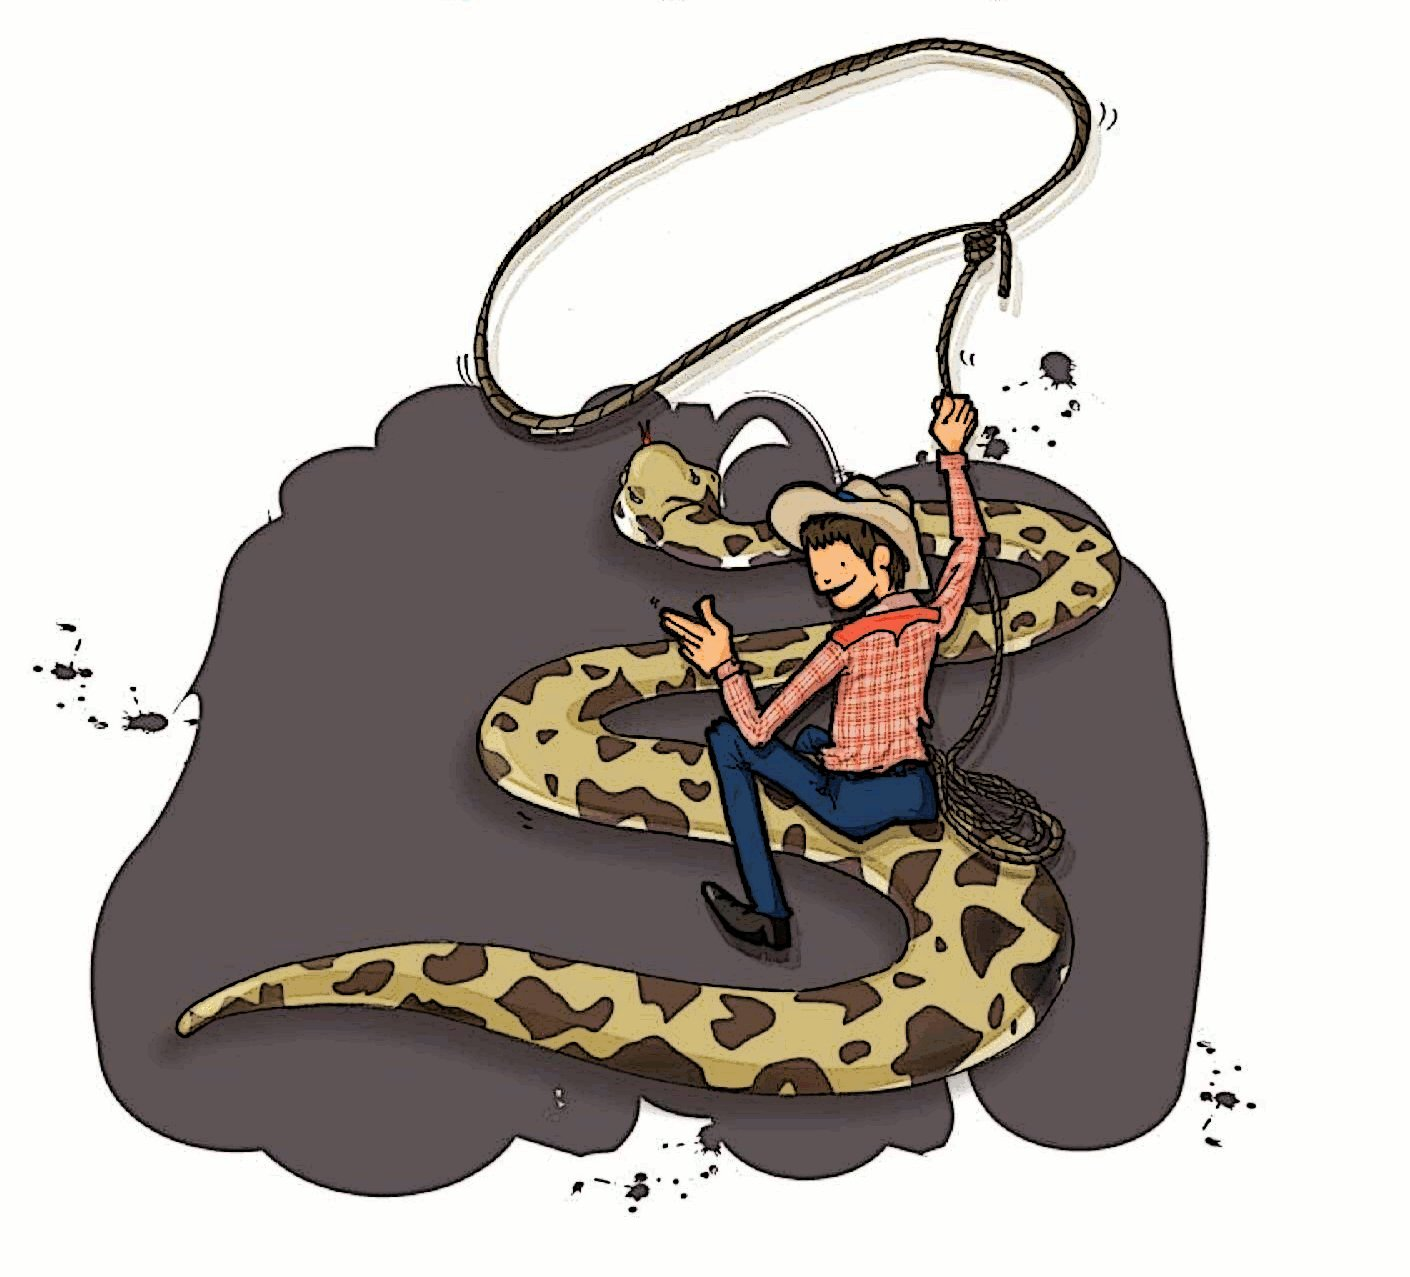
\includegraphics[width=19cm]{images/couv.jpg}
	% \vfill
	% }}} 
%\setmathfont{Linux Libertine O}
%\setmonofont[Mapping=tex-text]{DejaVu Sans Mono}
%\setmonofont[Mapping=tex-text]{Liberation Mono}
%\renewcommand{\tablemark}[1]{\markboth{ #1}{}}
% 
% \parindent 1cm
% \parskip 0.2cm
% \topmargin 0.2cm
% \oddsidemargin 1cm
% \evensidemargin 0.5cm
% \textwidth 15cm
% \textheight 21cm
% 
% \definecolor{PaleBlue}{rgb}{0.95,0.95,1}
% 
 \newenvironment{listing}
 {\begin{list}{}{\setlength{\leftmargin}{1em}}\item\footnotesize\samepage}
 {\end{list}}
 \newenvironment{listingignore}
 {\begin{list}{}{\setlength{\leftmargin}{1em}}\item\footnotesize\samepage}
 {\end{list}}

\def\appendixname{Annexe}%
\def\appendixautorefname{Annexe}%
 
 
% 
% \newcommand{\code}{\textcolor{OliveGreen}\bfseries}
% 
% \@FRONTCOVER_INC@version{FRONTCOVER}
% \@WINDOWS_INC@version{WINDOWS}
% \@MAC_INC@version{MAC}
% \@LINUX_INC@version{LINUX}
% 
% \title{Snake Wrangling for Kids - Learning to Program with Python}
% \author{Jason R Briggs}
\makeindex
\begin{document}

% This work is licensed under the Creative Commons Attribution-Share Alike 2.0 France License.
% To view a copy of this license, visit http://creativecommons.org/licenses/by-sa/2.0/fr/legalcode
% or send a letter to Creative Commons, 171 Second Street, Suite 300, San Francisco, California, 94105, USA.


\scalefont{0.8}
\ChNumVar{\fontsize{100}{100}\selectfont\textit} 
%\ChNameVar{\fontsize{5}{5}\selectfont\textrm} 
\ChTitleVar{\fontsize{28}{28}\selectfont\textrm}

\frontmatter

%\lstset{language=Python}
%\addfontfeature{Ligatures=Historical}

%\addfontfeature{Numbers=OldStyle}

\addfontfeature{Fractions=On}
\thispagestyle{empty}



\begin{center}
\textcolor{bleu}{\textbf{\fontsize{40}{40}\selectfont\textsf{Domptage de serpent pour les enfants}}}

\textcolor{bleu}{\textsf{\begin{Huge}Apprendre à programmer avec Python\end{Huge}}}

\vspace{1cm}

\begin{flushleft}
\textcolor{red}{\textsf{\begin{Huge}\Ovalbox{Édition Windows}\end{Huge}}}
\end{flushleft}

\AddToShipoutPicture*{
 \put(0,0){
 \parbox[b][\paperheight]{\paperwidth}{
 \vfill
 \vspace{2cm}
\begin{flushleft}
\hspace*{1cm}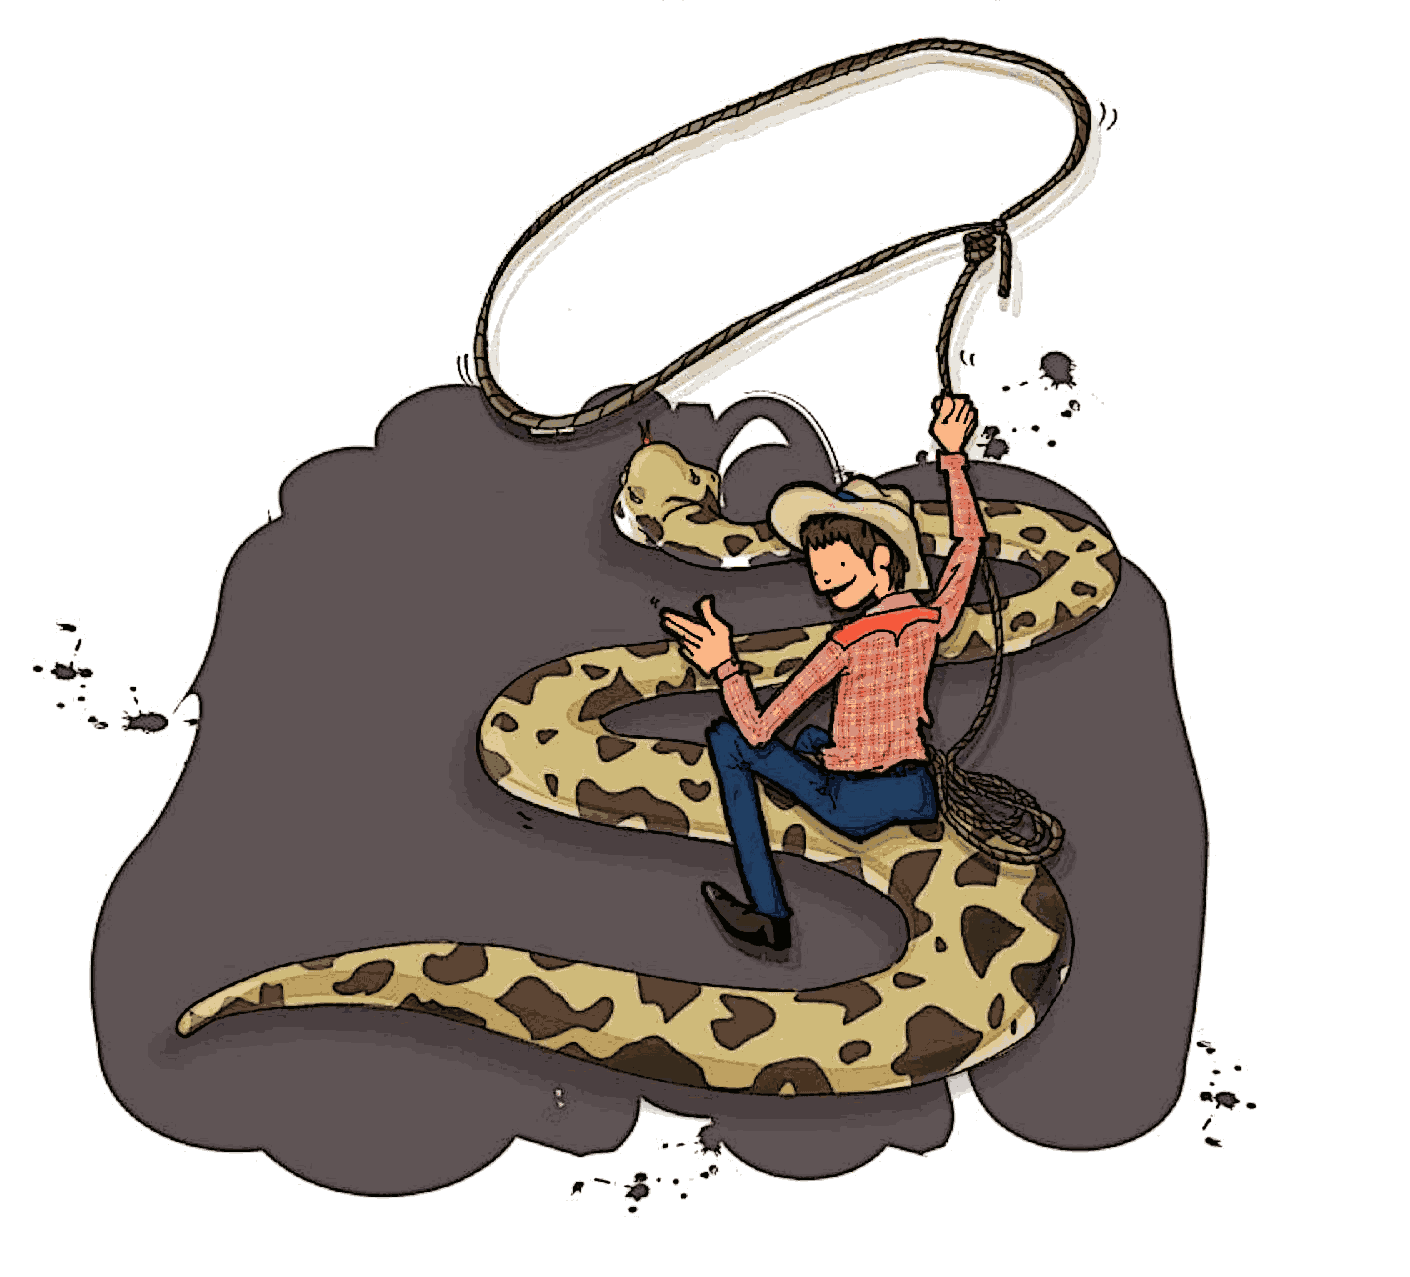
\includegraphics[width=21cm]{images/couv.png}
\end{flushleft}
 \vfill
 }}}

\vspace{16cm}

%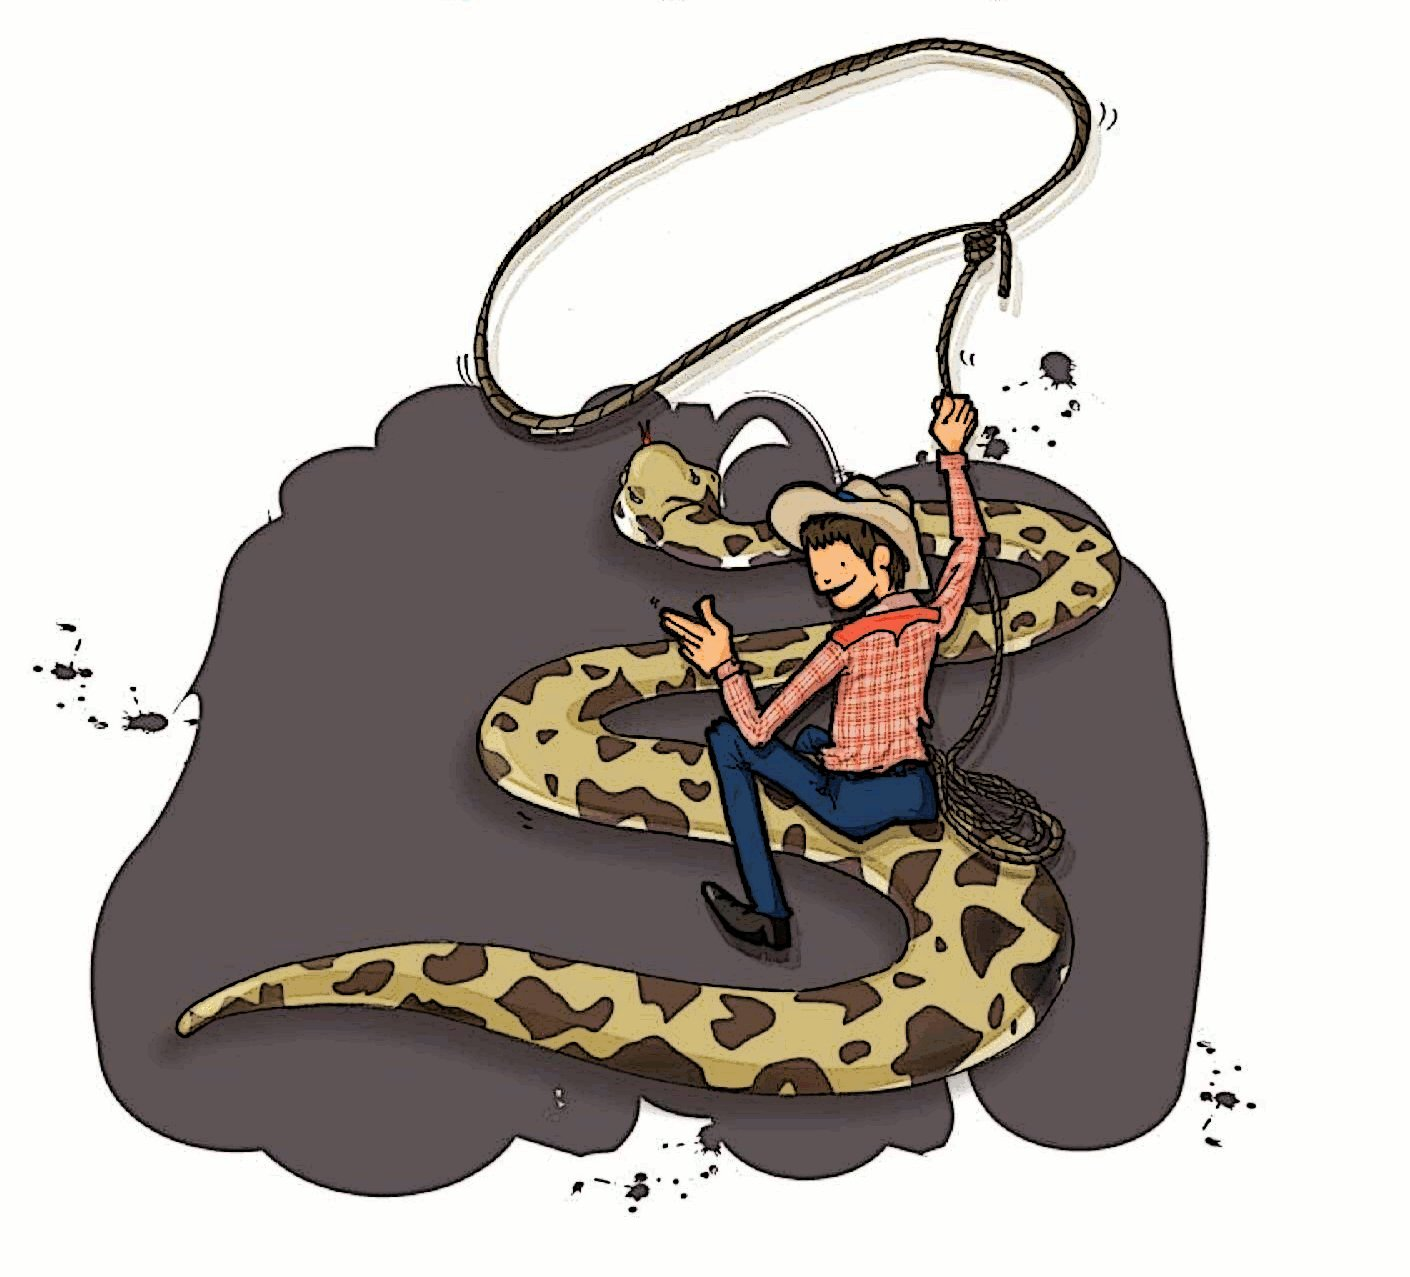
\includegraphics[scale=0.35]{images/couv.jpg} 
\end{center}

\begin{flushright}
\textcolor{bleu}{\begin{Huge}\textsf{Écrit par Jason R. Briggs}\end{Huge}}

\textcolor{bleu}{\begin{huge}\textsf{Traduit et adapté par Michel Weinachter}\end{huge}}
\end{flushright}

\newpage

\textit{Domptage de serpents pour les enfants, apprendre à programmer en Python}

par Jason R. Briggs

traduit et adapté par Michel Weinachter

\bigskip
Version: 0.7.6

Version française: 0.0.1

\bigskip
Copyright © 2007-2009

\bigskip
Publié par... ah, personne en fait.

\bigskip
Illustration de couverture par Nuthapitol C., illustrations par Nuthapitol C. et Michel Weinachter, cliparts:
\url{openclipart.org} et \url{commons.wikimedia.org}.

\bigskip
Composé avec \XeTeX{} et \XeLaTeX{} en utilisant les fontes \emph{Linux Libertine}, \textsf{Linux Biolinum}, \texttt{Computer Modern}, \setsansfont[Mapping=tex-text]{DejaVu Sans}\textsf{DejaVu} pour quelques symboles, et Firefly pour quatres caractères chinois {%\setromanfont[Mapping=tex-text]
\fontspec{AR PL UMing CN}漢字}.%\zhfont{漢字}.
 
\bigskip
Site web:

\url{http://www.briggs.net.nz/log/writing/snake-wrangling-for-kids}

\bigskip
Remerciements de l'auteur: merci à Guido van Rossum (pour la bienveillante dictature du langage Python), les membres de la liste de diffusion Edu-Sig (pour leurs avis et commentaires utiles) et à l'auteur David Brin (l'instigateur original de ce livre).

\bigskip
Remerciements du traducteur: merci à Jason R. Briggs, Gael Lickindorf, Anne, Christophe, Thaïs \& Anne-Sophie.

\bigskip
\begin{center}

%\begin{tabular}[t]{cc}
Licence:
%&


\includegraphics[scale=0.4]{images/CC-BY-SA.png}\\ 
%\end{tabular} 

\end{center}


Cette Œuvre est licenciée selon les termes du Contrat Public Creative Commons: 
Paternité-Partage des Conditions Initiales à l'Identique 2.0 France
Pour voir une copie de cette licence vous pouvez vous rendre à l'adresse suivante:
\url{http://creativecommons.org/licenses/by-sa/2.0/fr/}.

\bigskip

Vous êtes libres:
\begin{description}

\item[] 
\includegraphics[scale=0.2]{images/Share.pdf}\bf{} de reproduire\rm, distribuer et communiquer cette création au public
\item[] 
\includegraphics[scale=0.2]{images/remix.pdf}\bf{} de modifier\rm{} cette création
\end{description}

\bigskip
Selon les conditions suivantes:
\begin{description}
\item[] 
\includegraphics[scale=0.2]{images/Cc-by_new.pdf}\bf{} Paternité\rm{}. Vous devez citer le nom de l'auteur original de la manière indiquée par l'auteur de l'œuvre ou le titulaire des droits qui vous confère cette autorisation (mais pas d'une manière qui suggérerait qu'ils vous soutiennent ou approuvent votre utilisation de l'œuvre).
\item[] 
\includegraphics[scale=0.2]{images/sa.pdf} \textbf{Partage des Conditions Initiales à l'Identique}. Si vous modifiez, transformez ou adaptez cette création, vous n'avez le droit de distribuer la création qui en résulte que sous un contrat identique à celui-ci.
\end{description}
\begin{itemize}
\item À chaque réutilisation ou distribution de cette création, vous devez faire apparaître clairement au public
les conditions contractuelles de sa mise à disposition. La meilleure manière de les indiquer est un lien vers la
 page web:\\
\url{http://creativecommons.org/licenses/by-sa/2.0/fr/}.

\item Chacune de ces conditions peut être levée si vous obtenez l'autorisation du titulaire des droits sur cette œuvre.
\item Rien dans ce contrat ne diminue ou ne restreint le droit moral de l'auteur ou des auteurs.
\end{itemize}

\bigskip
Ce qui précède n'affecte en rien vos droits en tant qu'utilisateur (exceptions au droit d'auteur: copies réservées à l'usage privé du copiste, courtes citations, parodie...).

Une version complète du Contrat est disponible sur:\\
\url{http://creativecommons.org/licenses/by-sa/2.0/fr/legalcode}.

\scalefont{1.4}
\sommaire

%\clearpage
%\newpage
%\AddToShipoutPicture*{\BackgroundPicture}
%\phantom{a}
%\vspace{9cm}
% \begin{center}
%\fontsize{50}{50}\selectfont
%\textcolor{gray}{\XeTeX}
%\end{center}
%\vfill

%
% This work is licensed under the Creative Commons Attribution-Share Alike 2.0 France License.
% To view a copy of this license, visit http://creativecommons.org/licenses/by-sa/2.0/fr/legalcode
% or send a letter to Creative Commons, 171 Second Street, Suite 300, San Francisco, California, 94105, USA.



\markboth{}{}

\chapter{Préface}
\section*{\center{\textit{Une note aux parents...}}}

Chers parents et autres personnes attentionnées,\\

\section*{Vous vous demandez peut-être pourquoi apprendre à programmer?}
Apprendre à programmer permettra à votre enfant d'améliorer sa logique. Un ordinateur ne fait que ce qu'on lui a demandé. Si le programme ne fonctionne pas c'est que sa logique interne est mauvaise. 

De plus, savoir comment fonctionnent les ordinateurs permettra à l'enfant de comprendre qu'ils ne fonctionnent pas grâce à de la poudre magique mais grâce à la magie du génie humain.


\section*{Vous vous demandez peut-être, pourquoi Python?}
Python est un langage simple mais pas simpliste. Les commandes Python ont des rôles indépendants: «~il doit y avoir une manière évidente, de préférence une seule, de faire les choses~». Ces commandes sont donc en nombre limitées ce qui permet de se concentrer sur la logique du programme et non pas sur les commandes à utiliser. 
Néanmoins Python est puissant, d'ailleurs des organismes comme l'INRIA ou la NASA utilisent Python. Python est utilisé par des gouvernements pour des infrastructures critiques. Les entreprises l'utilisent comme Google qui fournit d'ailleurs un environnement Python en ligne.

Python est un langage de haut niveau qui ne contient pas de concepts liés au matériel ou au système d'exploitation ce qui permet de réaliser des programmes simples sans se focaliser sur des éléments non directement productifs. Python est interactif sa ligne de commande permet de réaliser des tests sans passer par des étapes complexes.

Par ailleurs, Python impose une écriture compréhensible car les différents blocs des programmes sont indiqués par les indentations du texte.

\bigskip
\section*{Comment installer Python?}
De manière à ce que votre enfant puisse commencer à programmer, vous avez besoin 
d'installer Python sur votre ordinateur. Ce livre a été récemment mis à jour pour Python~3.0; cette version de Python est la plus récente et n'est pas compatible avec les versions antérieures. Si vous avez une
version plus ancienne installée, vous devez télécharger la dernière version pour utiliser ce livre.\\


Installer Python est une tâche assez simple, mais il y a quelques différences selon le système d'exploitation que 
vous utilisez. 

Ce livre existe en trois versions: Linux, Mac Os X et Windows. La version que vous avez en main est la version Windows. Si vous n'utilisez pas Windows, vous pouvez télécharger la version adaptée sur:

\url{http://www.briggs.net.nz/log/writing/snake-wrangling-for-kids}.\\



Si vous venez juste d'acheter un nouvel ordinateur, que vous n'avez pas idée de quoi faire avec et que les phrases précédentes vous ont remplit de frissons glacés, vous devriez sûrement trouver quelqu'un pour faire ça pour vous.\\


Selon votre ordinateur et la vitesse de votre connexion à Internet, cette installation devrait vous prendre entre quelques minutes et plusieurs heures.

Premièrement, allez sur \url{www.python.org} et téléchargez le dernier installateur pour Python~3. À la date de l'écriture de ce livre vous pouvez le trouver à l'adresse \index{installation} \url{http://www.python.org/ftp/python/3.0.1/python-3.0.1.msi}.

Double-cliquez sur l'icône de l'installateur de Python pour Windows (vous vous rappelez où vous l'avez téléchargé, n'est-ce pas?), et suivez les instructions pour l'installer à l'endroit par défaut (qui est probablement \verb+C:\Python30+ ou quelque chose de très similaire).\\


\textit{Après l'installation...}


... Vous pourriez avoir besoin de vous asseoir à côté de votre enfant pour quelques premiers chapitres, mais 
heureusement après quelques exemples, il devrait chasser vos mains du clavier et faire les choses par lui-même. 
Il devrait, au moins, savoir comment utiliser un éditeur de texte quelconque avant de commencer (non, pas un traitement de texte comme Word, un vrai éditeur de texte à l'ancienne, sans gestion d'effets de style comme le bloc-notes) il devrait au moins être capable d'ouvrir et de fermer des fichiers, de créer des fichiers «~texte~» et sauvegarder ce qu'il fait. Mis à part ça, ce livre va essayer de lui enseigner le \textit{b+a, ba} à compter de cette page.

\bigskip
Merci pour votre temps, bien cordialement.\\
%\AddToShipoutPicture*{\BackgroundPicture}


\textit{Le Livre}
\pagestyle{headings}
\pagenumbering{arabic}

% This work is licensed under the Creative Commons Attribution-Share Alike 2.0 France License.
% To view a copy of this license, visit http://creativecommons.org/licenses/by-sa/2.0/fr/legalcode
% or send a letter to Creative Commons, 171 Second Street, Suite 300, San Francisco, California, 94105, USA.


\mainmatter
\clearemptydoublepage
\chapter{Tous les serpents ne vont pas vous mor\-dre}
\section{Bonjour, je suis votre livre}
Il y a des chances que vous\footnote{Mon traducteur a fait le choix de traduire «~you~» par vous, le voussoiement lui semble plus adapté que le tutoiement généralisé dans certains livres pour enfants.} ayez reçu ce livre pour votre anniversaire. Tante Gertrude allait vous donner des chaussettes disparates qui auraient été deux tailles trop grandes (et que vous n'auriez pas porté plus grand de toute manière). À la place, elle a entendu quelqu'un parler de ce livre à imprimer, s'est rappelée que vous aviez un de ces ordinateurs-machin-chose, que vous aviez essayé de lui monter comment l'utiliser au dernier Noël (vous aviez abandonné quand elle avait commencé à parler à la souris), et l'a fait imprimer.
\\


\emph{Soyez juste soulagés que vous n'ayez pas eu ces vieilles chaussettes moisies.\\}


J'espère que vous n'avez pas été trop désappointé quand j'ai jailli à leur place du papier recyclé d'emballage.
Un livre qui ne parle pas vraiment (O.K., qui ne parle pas du tout), avec un titre de mauvaise augure sur la couverture 
qui parle d'«~apprendre...~». Mais prenez un moment pour penser à ce que je ressens. Si vous étiez un personnage d'un roman qui parle de magiciens et que j'étais dans la bibliothèque de votre chambre, j'aurais probablement des dents... ou peut-être des yeux verts. Je pourrais contenir des images animées ou être capable de faire des hurlements de fantôme quand vous ouvreriez mes pages. À la place, je suis imprimé sur des feuilles de papier A4 cornées, agrafées ensemble ou peut-être mises dans une chemise. Comme pourrais-je le savoir? Je n'ai pas d'yeux.\\


\emph{Je donnerai n'importe quoi pour une belle mâchoire pleine de dents aiguisées...}\\


Malgré tout n'est pas aussi catastrophique qu'il y parait. Même si je ne peux pas parler... Ou mordre vos doigts quand vous ne regardez pas... Je peux vous parler un petit peu de ce qui fait fonctionner les ordinateurs. Pas la partie physique, avec les fils, les puces, les câbles et les éléments qui pourraient plus que probablement vous électrocuter aussitôt que vous les toucheriez (donc ne le faites pas!) mais la partie cachée qui court à l'intérieur de ces fils, ces puces, ces câbles et ces machins qui font que les ordinateurs sont vraiment utiles. 

\begin{center}
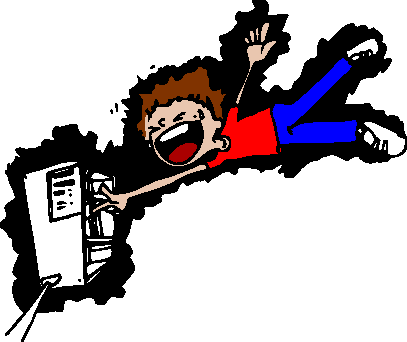
\includegraphics[scale=1]{images/electrocution.pdf} 
\end{center} 

C'est un petit peu comme les pensées qui tournent dans votre tête. Si vous n'aviez pas de pensée, vous seriez assis sur le sol de votre chambre, regardant vaguement vers la porte et bavant sur l'avant de votre t-shirt. Sans programme, les ordinateurs seraient seulement utiles comme des cales-porte --- et même comme cela ils ne seraient pas très utiles parce que vous devriez prendre garde à bien les enjamber pendant la nuit. Et il n'y a rien de pire que de se cogner un orteil dans l'obscurité.

\bigskip
\emph {Je suis juste un livre et même moi je sais ça.}

\bigskip
Votre famille a peut-être une Playstation, une Xbox ou une Wii qui trônent dans le salon. Elles ne seraient que d'une faible utilité sans programme (jeu) pour les faire fonctionner. Les lecteurs de DVD, certains réfrigérateurs et même la plupart des voitures, ont tous des programmes informatiques qui les rendent plus utiles qu'ils ne pourraient l'être autrement. Votre lecteur de DVD utilise des programmes pour jouer des disques; votre réfrigérateur peut disposer d'un programme simple pour s'assurer qu'il n'utilise pas trop d'électricité, mais continue de garder les aliments froids; certaines voitures peuvent avoir un ordinateur avec un programme pour avertir si elles risquent d'avoir un accident.

Si vous savez comment écrire un programme informatique, vous pouvez faire toutes sortes de choses utiles, comme programmer vos propres jeux ou créer vos propres pages web qui peuvent réagir au lieu d'un bête machin coloré. Être capable de programmer pourrait peut-être même vous aider dans votre travail scolaire.
\\


Cela dit, passons maintenant à un sujet un peu plus intéressant.

\section{Qu'est ce que nous allons voir?}
Nous allons voir comment poser des questions et prendre en compte la réponse: par exemple demander à quelqu'un son nom et lui faire des remarques sur celui-ci.

Nous allons aussi voir comment faire faire des dessins comme sur la \autoref{fig:pythonimage}.

\begin{figure}[!ht]
\capstart
\centering
\subfigure[Le Yin et le Yang]{

\includegraphics[scale=0.6]{images/yinyang_bis}
\label{fig:yinyang_bis}
}
\subfigure[Étoile à neuf branches]{

\includegraphics[scale=0.5]{images/etoileorange3}
\label{fig:etoileorange3}
}
\caption{Des dessins faits avec Python}\label{fig:pythonimage}
\end{figure}

Nous verrons aussi comment afficher un message de bienvenue différent tous les jours.

\section{Quelques mots à propos des langages}
Comme les humains, certainement les baleines, possiblement les dauphins et peut-être même les parents (même si cela fait débat pour ces derniers), les ordinateurs ont leur propre langage. En fait, aussi comme les humains, ils ont plus d'un langage. A, B, C, D et E ne sont pas juste des lettres, ce sont aussi des langages de programmation (ce qui prouve que les adultes n'ont pas d'imagination et devraient lire soit un dictionnaire soit un répertoire avant de nommer quoique ce soit). Oh et si vous ajoutez quelques plus ou dièses (+, \#) après certaines de ces lettres que je viens de lister, il s'agit encore de langages de programmations qui sont presque les mêmes et n'en diffèrent que légèrement.

D'autres sont nommés d'après des personnes, en utilisant de simples acronymes (les premières lettres d'une série de mots), voir pour certains à partir d'une émission de télévision. 

\bigskip
\emph{Qu'est-ce que je vous avez dit? Pas d'imagination!}

\bigskip
Par chance, de nombreux langages sont tombés en désuétude ou ont disparu complètement; mais la liste des différentes manières de «~parler~» à un ordinateur reste vraiment ennuyeusement longue. Je vais seulement parler d'un de ceux-ci --- sinon nous ferions aussi bien de ne pas commencer.\\


Il serait alors plus productif de vous asseoir dans votre chambre et de baver sur le devant de votre t-shirt.

\section{L'ordre des serpents constricteurs non-venimeux...}
... ou pythons, pour faire plus court.

\bigskip
Le python est un serpent mais le Python est un langage de programmation. Néanmoins, son nom ne vient pas directement du reptile sans patte; il s'agit d'un de ces rares langages de programmations nommés d'après une émission de télévision. Le Monty Python's Flying Circus était une émission humoristique britannique populaire durant les années 1970 (et en fait, encore vraiment populaire actuellement) qui nécessite d'avoir un certain âge pour la trouver amusante. Toute personne en dessous de... disons douze ans... pourrait se demander d'où peut provenir tout ce battage\footnote{Mis à part «~the fish slapping dance~» ou danse tape-poisson qui est drôle quelque soit votre âge.}.

Il y a un certain nombre de choses à propos de Python (le langage de programmation, pas le serpent ou l'émission de télévision) qui le rende extrêmement pratique quand vous allez apprendre à programmer. Pour nous, en ce moment l'important est que vous puissiez commencer et faire des choses vraiment rapidement.

C'est maintenant la partie où vous espérez que Maman, Papa ou quiconque est en charge de l'ordinateur, a lu la partie au début de ce livre nommée «~Une note aux parents...~».

\begin{figure}[!ht]
\capstart
\centering
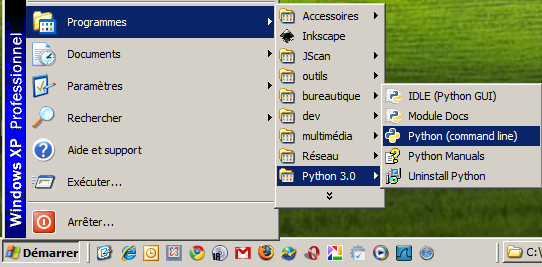
\includegraphics[scale=0.6]{images/startmenu}
\caption{Python dans le menu de Windows.}\label{fig:startmenu}
\end{figure}

Il y a une bonne manière de vérifier s'ils l'ont réellement lu: cliquez sur le bouton «~démarrer~» en bas à gauche de l'écran, cliquez sur «~Programmes~» (qui doit avoir un petit triangle à coté), et avec optimisme dans la liste des programmes vous devriez voir «~Python 3.1~» (ou quelque chose approchant).\index{console}
 
La figure \ref{fig:startmenu} montre ce que vous devriez voir. Cliquez sur «~Python (command line)~» et vous devriez voir quelque chose comme sur la figure \ref{fig:pycl}.

\begin{figure}[!ht]
\centering
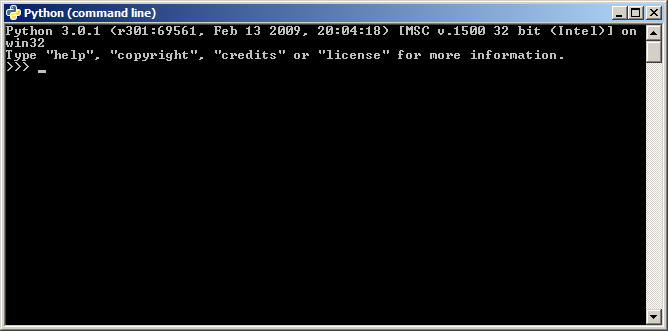
\includegraphics[scale=0.6]{images/pycl}
\caption{Ligne de commande Python sous Windows.}\label{fig:pycl}
\end{figure}

La ligne de commande Python fonctionne sous Windows à partir de la ligne de commande Windows et hérite de certaines limitations en particulier pour l'affichage de certains caractères (typiquement les caractères français comme «~œ~» ou  «~\begin{small}\euro\end{small}~» qui seront remplacés par des «~\texttt{?}~») sans que cela ne pose de problème important.

Cliquez sur «~IDLE (Python GUI)~» et vous devriez voir quelque chose comme sur la figure \ref{fig:shell}.

\begin{figure}[!ht]
\centering
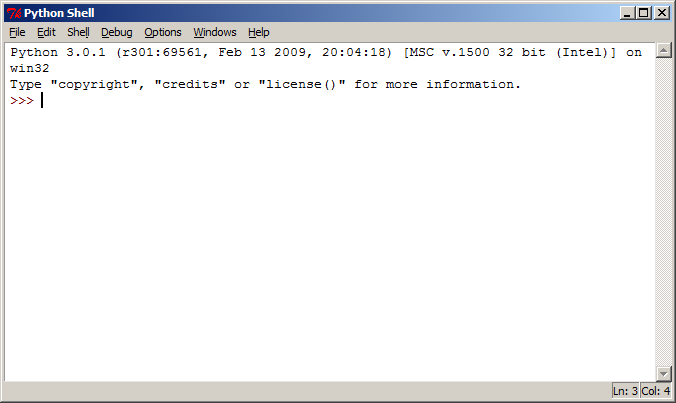
\includegraphics[scale=0.6]{images/shell}
\caption{Shell Python sous Windows.}\label{fig:shell}
\end{figure}

Le shell\footnote{Le mot \emph{shell} signifie en anglais coquille, c'est le nom donné à l'interface d'un système d'exploration, c'est à dire la partie que manipule l'utilisateur pour utiliser un système d'exploitation. Par extension, ce nom est donné à certaines autres interfaces.} Python est plus puissant et plus convivial: en particulier il met en valeur en les coloriant les éléments clef des commandes qui sont passées ce qui limite le risque d'erreur.

\section*{Si vous découvrez qu'ils n'ont pas lu la section du début...}

... parce que s'il manque quelque chose quand vous essayez de suivre ces instructions --- alors retournez au début du livre et brandissez le sous leur nez alors qu'ils essayent de lire le journal, et soyez plein d'optimisme. Si vous avez du mal à les convaincre de s'extraire du canapé, dire: «~s'il-vous-plait, s'il-vous-plait, s'il-vous-plait...~» encore et encore jusqu'à ce que cela devienne ennuyant devrait vraiment bien fonctionner. Bien sûr, l'autre chose que vous pouvez faire est de retourner au début du livre et suivre les instructions de la préface pour installer Python vous même.

\section{Votre premier programme en Python}

Avec de la chance, si vous avez atteint ce point, vous avez réussi à démarrer la console Python, qui est un moyen de lancer des commandes Python et des programmes. Quand vous lancez la console (ou après avoir entré une commande), ce que vous voyez en premier est appelé une «~invite de commande~» (invite pour faire court ou «~\emph{prompt}~» en anglais). 
Dans la console Python, l'invite est matérialisée par trois chevrons, ou trois symboles plus-grand-que (\verb+>+) pointant vers la droite:
\begin{Verbatim*}[frame=single,rulecolor=\color{gray}, label=ne pas saisir]
>>>
\end{Verbatim*}
Si vous placez suffisamment de commandes Python ensembles, vous avez un programme que vous pouvez lancer même en dehors de la console... Mais pour le moment nous allons garder les choses simples et taper nos commandes directement dans la console, à l'invite (\verb+>>>+).
\VerbatimFootnotes
Ainsi pourquoi ne pas commencer à taper ce qui suit
\footnote{Le \verb*+ + dans les codes symbolise \emph{une} espace, c'est à dire le caractère issu de l'appui sur la barre d'espace. Quand cela est utile, ce symbole sera affiché.}:

\begin{Verbatim*}[frame=single,rulecolor=\color{mbleu}, label=à taper]
print("Bonjour le monde !")
\end{Verbatim*}

Note du traducteur: la plupart des langages de programmation utilisent des mots clefs en anglais. Python ne fait pas exception à la règle. Vous avez donc l'occasion d'apprendre quelques mots d'anglais en plus d'un langage de programmation. Le verbe «~\emph{(to) print}~» signifie en anglais «~imprimer~» ou «~afficher~» du moyen anglais \emph{prente} issu du participe passé \emph{preint, prient} du verbe \emph{priendre}, du latin \emph{premere} qui signifie presser. Par la suite les explications et traductions des mots anglais seront mises en note de bas de page.\\

Pour information les extraits de code sont mis en valeur dans des cadres colorés. 
Les cadres bleus contiennent des exemples que vous pouvez taper sans difficulté particulière:

\begin{Verbatim}[frame=single,rulecolor=\color{mbleu}, label=à taper]

\end{Verbatim}

Python est résistant: les erreurs que vous pourriez obtenir sont sans gravité, vous pouvez expérimenter sans peur.
Il vous sera même indiqué parfois des tests à réaliser pour le pousser à la faute. Python couinera un peu, mais ce n'est pas grave.


\begin{center}
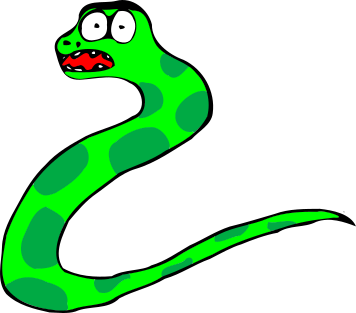
\includegraphics[scale=0.5]{images/serpent}
\end{center}

Les cadres rouges contiennent des erreurs, si vous les tapez vous obtiendrez le message d'erreur indiqué:

\begin{Verbatim}[frame=single,rulecolor=\color{red}, label=erreur]

\end{Verbatim}

Les cadres verts contiennent des exemples valides mais avec des subtilités qui viennent d'être expliquées ou qui vont l'être prochainement, si vous les tapez en oubliant des espaces (symbolisée par \verb*+ +) vous pouvez obtenir des messages d'erreur:

\begin{Verbatim*}[frame=single,rulecolor=\color{green}, label=à taper avec attention]
 
\end{Verbatim*}
Les cadres gris contiennent des exemples qui ne sont pas à taper:

\begin{Verbatim}[frame=single,rulecolor=\color{gray}, label=ne pas saisir]
 
\end{Verbatim}


Assurez-vous d'inclure les guillemets (ceux qui sont comme cela \texttt{" "}), et d'appuyer sur entrée à la fin de la ligne.
Normalement vous devriez avoir quelque chose comme:

\begin{Verbatim*}[frame=single,rulecolor=\color{mbleu}, label=à taper si cela n'est pas déjà fait]
>>> print("Bonjour le monde !")
Bonjour le monde
\end{Verbatim*}


L'invite réapparaît pour vous faire savoir que la console Python est prête à accepter plus de commandes.
\\


Félicitations! Vous venez juste de créer votre premier programme en Python. La commande \index{print}«~\verb+print+~» est une fonction qui écrit tout ce qui est entre les parenthèses sur la sortie de la console, nous la verrons plus en détail ultérieurement.

\section{Votre second programme Python... Le même à nouveau?}

Les programmes Python ne seraient pas très utiles si vous aviez à taper les commandes chaque fois que vous voulez faire quelque chose, ou si vous écriviez un programme pour quel\-qu'un et qu'il avait à le taper avant qu'il ne puisse l'utiliser.

Le traitement de texte, que vous pouvez utiliser pour faire des dossiers pour l'école, est probablement constitué de dix à cent millions de lignes de code. Selon le nombre de lignes imprimées sur une page et même si vous imprimez sur les deux faces, cela représente quatre cents mille pages imprimées, ou une pile de quarante mètres de haut. Imaginez-vous juste quand vous ramenez un tel logiciel à la maison depuis le magasin, il faudrait plus que quelques voyages pour ramener autant de papier. Et vous feriez mieux d'espérer qu'il n'y ait pas une rafale de vent quand vous ramenez les piles de papier.

\begin{center}

\includegraphics[scale=1]{images/encore.pdf} 
\end{center} 

Heureusement il y a une alternative à toute ces saisies de texte\footnote{On parle aussi de dactylographie, écriture avec les doigts.} ou rien ne serait jamais fini.
Ouvrez le «~Bloc-notes~» (cliquez sur «~Démarrer~», «~Programmes~» et vous devriez le trouver dans le sous menu «~Accessoires~») et tapez la commande exactement comme vous l'aviez tapée dans la console auparavant:

\begin{Verbatim}[frame=single,rulecolor=\color{gray}, label=ne pas saisir]
print("Bonjour le monde !")
\end{Verbatim}
\rm

Cliquez sur le menu «~Fichier~» (dans le Bloc-notes) puis sur «~Enregistrer~», il vous sera alors demandé de choisir un nom de fichier, entrez «~\texttt{bonjour.py}~» et sauvez le fichier sur le Bureau. Pour ce faire cliquez sur l'icône «~\texttt{Bureau}~», changez le type de «~\texttt{Fichiers texte (*.txt) en «~\texttt{Tous les fichiers}~» }~», puis changer le «~\texttt{*.txt}~» en «~\texttt{bonjour.py}~». Double cliquez sur l'icône bonjour.py sur votre bureau (voir figure \ref{fig:bureau} et pendant un bref instant une fenêtre noire va apparaître.

\begin{figure}[!ht]
\centering
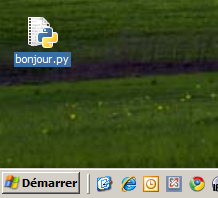
\includegraphics[scale=0.6]{images/bureau}
\caption{Programme Python sur le bureau.}\label{fig:bureau}
\end{figure}

Elle va disparaître trop rapidement pour que vous puissiez la lire mais «~Bonjour le monde !~» est apparu dans la fenêtre une fraction de seconde; nous y reviendrons plus tard et nous montrerons que le texte s'y est bien imprimé.

Ainsi, nous venons de voir que les sympathiques personnes qui ont créé Python, nous ont gentiment prémuni d'avoir à taper la même chose encore et encore et encore et encore... Comme le faisait certains dans les années 1980. Non, je suis sérieux, certains l'ont fait. Allez demander à votre maman ou votre papa s'ils n'ont pas possédé un MO5 ou un Amstrad CPC\footnote{Ces ordinateurs étaient populaires dans les années 1980 dans les pays francophones.} quand ils étaient plus jeunes. S'ils en ont eu un vous pouvez les montrer du doigt et rigoler.\\


Croyez moi sur ce point, vous ne comprendrez peut-être pas mais, eux, ils comprendront.\\

\emph{Soyez néanmoins prêts à courir.}\\


Mon cousin, le livre en version anglaise, parle de ZX81\footnote{Le Sinclair ZX81, vendu dans les années 1980 a été un des premiers ordinateurs vraiment abordable. Un grand nombre de jeunes garçons et de jeunes filles ont été complètement passionnés et tapaient les codes de jeux imprimés dans des magazines populaires consacrés au ZX81 pour découvrir après des heures de dactylographie que ces saletés ne fonctionnaient jamais correctement.} un ordinateur qui a été très populaire dans les pays anglo-saxons.


\section*{La fin du début}

Bienvenue dans le monde merveilleux de la programmation. Nous avons commencé vraiment simplement avec une 
application «~Bonjour le monde~»\footnote{«~Hello world~» en anglais}. tout le monde commence avec cela quand on apprend à programmer. Dans le prochain chapitre nous commencerons à faire des choses plus utiles avec la console Python et alors nous regarderons comment faire un programme.

 \vfill
\begin{center}
 
\includegraphics[width=5cm]{images/python.pdf}
\end{center}
 \vfill

\newpage
\thispagestyle{empty}
\AddToShipoutPicture*{
 \put(0,0){
 \parbox[b][\paperheight]{\paperwidth}{
 \vfill
\begin{center}
 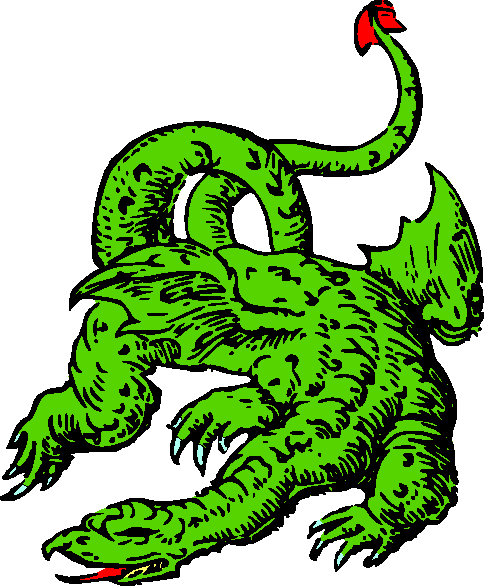
\includegraphics[width=5cm]{images/python_det.pdf}
\end{center}
 \vfill
 }}}

\include{8multipliés}

% This work is licensed under the Creative Commons Attribution-Share Alike 2.0 France License.
% To view a copy of this license, visit http://creativecommons.org/licenses/by-sa/2.0/fr/legalcode
% or send a letter to Creative Commons, 171 Second Street, Suite 300, San Francisco, California, 94105, USA.


\chapter{Tortues et autres choses lentes\label{chap:tortue1}}
\section{Un reptile plus lent que Python}
Il y a certaines similarités entre les tortues du monde réel et une tortue Python.
Dans le monde réel, une tortue   est un reptile, parfois vert, qui se déplace très lentement et porte sa maison sur le dos. Dans le monde de Python, une tortue est une petite flèche noire qui se déplace lentement dans une fenêtre. Néanmoins il n'est nulle part fait mention d'une maison.\\

En fait, considérant le fait que la tortue Python laisse une trace derrière elle dans la fenêtre, cela en fait moins une tortue qu'un petit escargot ou une limace. Néanmoins, je suppose qu'un module appelé «~limace~»  n'aurait pas été très attirant. C'est pour cela qu'il était plus sensé de garder les tortues. Il suffit d'imaginer une tortue qui transporterait quelques feutres et qui dessinerait en avançant.\\

Dans un passé lointain et sombre il y avait un simple langage de programmation appelé Logo. Logo était utilisé pour contrôler une tortue robot (appelé Irving). Au cours du temps la tortue a évolué depuis un robot qui pouvait se déplacer sur le sol à une petite flèche qui peut se déplacer sur l'écran.\\

\emph{Ce que revient à montrer que les choses ne s'améliorent pas tout le temps avec les avancés de la technologie. Une petite tortue robot aurait été nettement plus drôle.}\\

\section{À la recherche de la tortue perdue}

Le module «~\texttt{turtle\footnote{Le mot \emph{turtle} signifie tortue en anglais et semble venir du français.}}~» de Python est juste un petit peu comme la tortue Logo.
Nous verrons plus tard ce qu'est un module, mais 
pour le moment pensez juste que c'est quelque chose.

Néanmoins, Python a de nombreuses autres capacités que Logo. Le module «~\texttt{turtle}~» est une manière pratique 
 d'apprendre comment les ordinateurs tracent des images sur votre écran.\\

Bon commençons et voyons juste comment cela fonctionne. La première étape est de dire à Python que nous voulons utiliser «~\texttt{turtle}~» en important le module:

\begin{figure}[ht]
\begin{minipage}{0.4\linewidth}
\scalefont{1.1}
La gestion des fenêtres de Windows, différente de celle des autres systèmes d'exploitation, empêche de laisser le shell Python et la fenêtre «~\texttt{turtle}~» se recouvrir sans dysfonctionnement. En effet, si le shell Python et la fenêtre «~\texttt{turtle}~» se recouvrent une seule fenêtre verra son contenu mis à jour. Pour contourner ce problème, vous pouvez utiliser la ligne de commande Python ou réduire la largeur de la fenêtre du shell Python.\\

Vous pouvez voir sur la figure \ref{fig:shellami} le shell Python dont la largeur a été réduite de manière à empêcher le recouvrement.\\

Si le shell n'est pas assez réduit et que la fenêtre «~\texttt{turtle}~» et le shell sont superposées, il suffit de les déplacer ou de les redimensionner.
\end{minipage}
\hspace{0.5cm}
\begin{minipage}{0.5\linewidth}
\centering
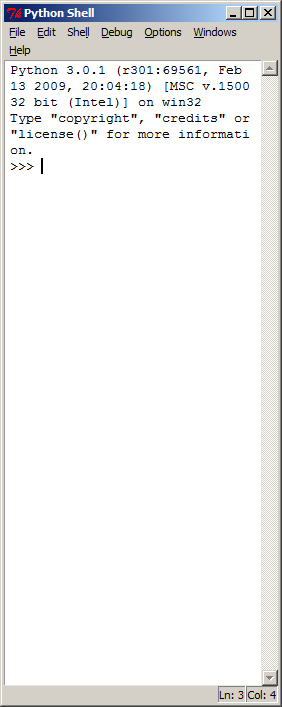
\includegraphics[scale=0.5]{images/shell_pour_turtle.png}
\caption{Shell Python redimensionné pour utiliser turtle}
\label{fig:shellami}
\end{minipage}
\end{figure}

Pour importer le module turtle faites:

\begin{Verbatim}[frame=single,rulecolor=\color{mbleu}, label=à taper]
>>> import turtle
\end{Verbatim}

Puis nous avons besoin d'afficher une feuille pour dessiner. Cette feuille est appelée en informatique zone de dessin. Cette zone de dessin est comme la toile qu'un artiste utilise pour peindre, dans notre cas c'est juste un espace blanc pour dessiner:

\begin{Verbatim}[frame=single,rulecolor=\color{mbleu}, label=à taper]
>>> tortue = turtle.Pen()
\end{Verbatim}

Attention Python fait la différence entre les minuscules et les capitales\footnote{On dit qu'il est sensible à la casse.}, il convient d'écrire «~\texttt{Pen\footnote{Le mot \emph{pen} signifie stylo, du vieux français \emph{penne} lui même du latin tardif \emph{penna} signifiant plume.
}}~»  et non pas «~\texttt{pen}~». Si vous vous êtes trompés retapez juste: «~\texttt{tortue = turtle.Pen(}~».


Quand nous voulons quitter «~\texttt{turtle}~» il est conseillé de fermer au préalable la zone de dessin en faisant «~\texttt{turtle.bye()}~».

\begin{Verbatim}[frame=single,rulecolor=\color{mbleu}, label=à taper]
>>> turtle.Pen()
\end{Verbatim}


Dans \verb+tortue = turtle.Pen()+ nous appelons une fonction particulière (Pen) du module turtle qui crée automatiquement une zone de dessin dans laquelle nous pouvons écrire et nous faisons pointer une variable vers le résultat de cette fonction de manière à pouvoir dessiner.

Une fonction est un bout de code réutilisable (à nouveau nous étudierons  les fonctions plus tard) qui fait quelque chose qu'il est utile de faire plusieurs fois. Dans notre cas la fonction «~\texttt{Pen}~» retourne un objet qui 
représente notre tortue (enfin notre flèche en forme de tortue). Nous associons cet objet à la variable «~\texttt{tortue}~».

Quand nous tapons le code dans la console Python, nous voyons une zone blanche apparaître (la zone de dessin dite \emph{canvas\footnote{Le mot \emph{canvas} signifie toile en anglais du français canevas.}} en programmation) qui ressemble à la figure \ref{fig:turtledebut}

\begin{figure}[ht!]
\centering
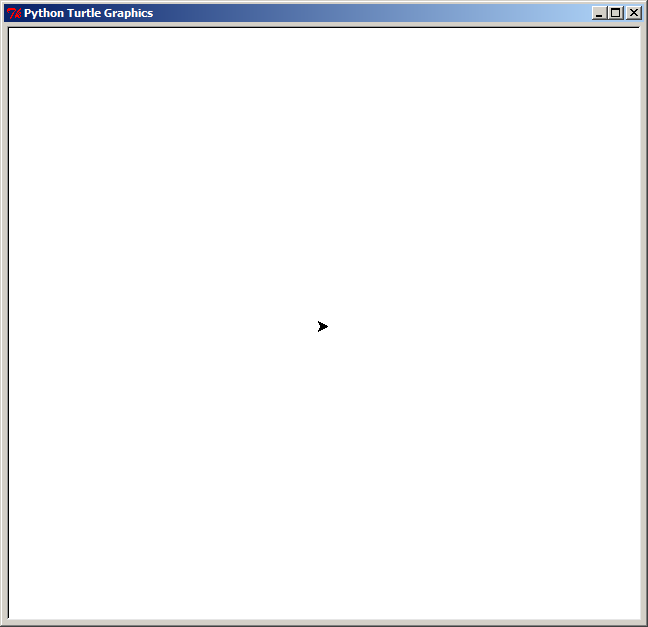
\includegraphics[scale=0.4]{images/turtle_debut.png}
\caption{Une flèche représente la tortue}
\label{fig:turtledebut}
\end{figure}

\emph{Oui la petite flèche au milieu de l'écran est notre tortue. Et non, elle ne ressemble pas vraiment à une tortue.}\\

La \emph{Fausse Bonne Idée} serait de faire :

\begin{Verbatim}[frame=single,rulecolor=\color{red}, label=erreur]
>>> turtle.Pen()
\end{Verbatim}

La zone de dessin serait créée mais sans étiquette pour identifier le stylo nous ne pourrions pas dessiner dessus.\\


Vous pouvez envoyer des instructions à la tortue, en utilisant des fonctions sur cet objet que nous venons de créer en appelant «~\texttt{turtle.Pen}~». Comme nous avons assigné cet objet à la variable tortue, nous utilisons «~\texttt{tortue}~» pour envoyer des instructions. Une instruction de notre tortue est «~\texttt{forward\footnote{Le mot \emph{forward} vers l'avant du vieil anglais foreweard,  \emph{fore} (avant) + \emph{-weard -ward} (suffixe de mouvement).}}~».

L'instruction «~\texttt{forward}~» dit à notre tortue d'avancer vers l'avant quelque soit la direction vers laquelle elle pointe. Disons à la tortue l'avancer vers l'avant de 50 \emph{pixels} (nous allons parler des pixels dans une minute):

\begin{Verbatim}[frame=single,rulecolor=\color{mbleu}, label=à taper]
>>> tortue.forward(50)
\end{Verbatim}

Vous devriez obtenir quelque chose qui ressemble à la figure \ref{fig:50px}.

\begin{figure}[h!]
\centering
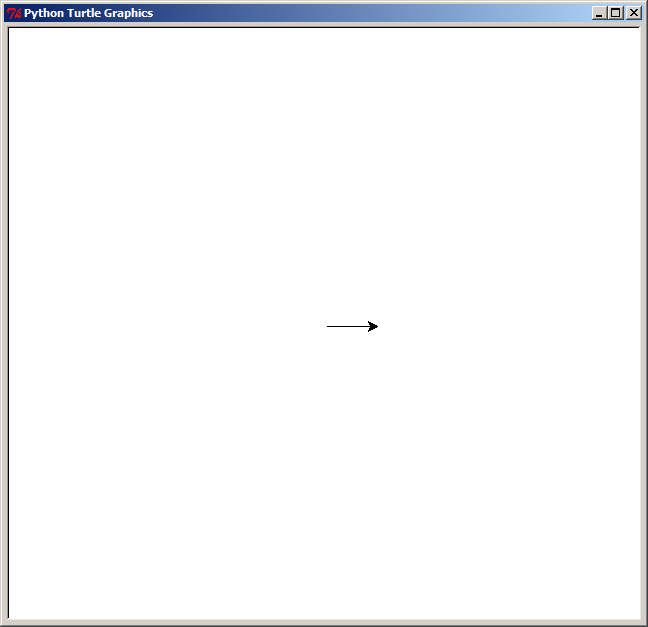
\includegraphics[scale=0.4]{images/50px.png}
\caption{La tortue dessine une ligne}
\label{fig:50px}
\end{figure}

Du point de vue de la tortue elle a avancé de cinquante pas. De notre point de vue elle s'est déplacée  de 50 pixels.\\


\emph{Bon qu'est-ce que qu'un pixel?}\\

Un pixel est un point sur l'écran. Quand vous regardez l'écran de votre ordinateur tout est fait de petits points (approximativement) carrés. Les programmes que vous utilisez, et les jeux auxquels vous jouez sur l'ordinateur ou votre console, sont faits d'une multitude de différents points colorés arrangés sur l'écran. En fait si vous regardez l'écran avec une loupe vous devriez être capable de voir de quoi sont faits ces points. Ainsi si nous zoomons dans la zone de dessin au niveau de la ligne qui vient d'être tracée par la tortue, nous pouvons voir que la flèche qui représente la tortue est aussi un paquet de points carrés, comme vous pouvez le voir sur la figure \ref{fig:points}.

\begin{figure}[h!]
\centering
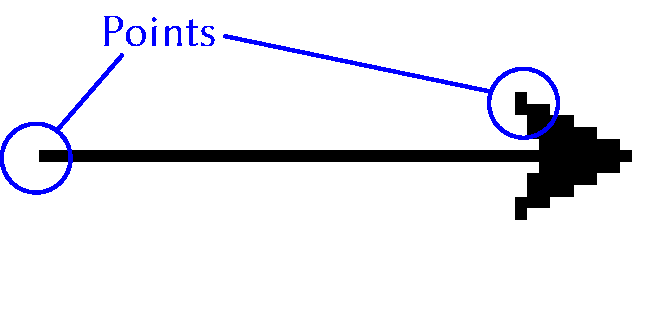
\includegraphics[scale=1]{images/points.pdf}
\caption{Zoom sur la tortue}
\label{fig:points}
\end{figure}

Nous parlerons plus de ces points, ou pixels, dans un prochain chapitre.
Maintenant nous allons dire à la tortue de tourner à gauche ou à droite:

\begin{Verbatim}[frame=single,rulecolor=\color{mbleu}, label=à taper]
>>> tortue.left(90)
\end{Verbatim}

L'instruction «~\texttt{left(90)\footnote{Le mot \emph{left} signifie gauche en anglais, du vieil allemand \emph{lucht} (gauche).}}~»  dit à la tortue de tourner vers la gauche de 90 degrés (souvent notés °). Vous n'avez peut-être pas encore appris ce que sont les degrés à l'école mais la manière la plus simple de se les représenter est qu'ils sont un peu comme les divisions d'une montre (voir la figure \ref{fig:clock}).
\begin{figure}[H]
\centering
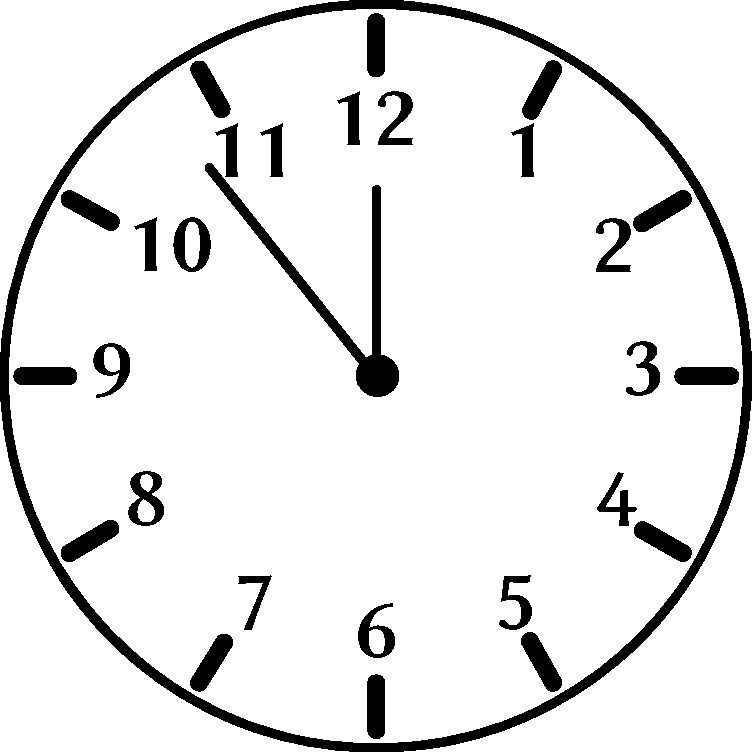
\includegraphics[scale=0.5]{images/clock.pdf}
\caption{Le cadran d'une montre et ses divisions}
\label{fig:clock}
\end{figure}

Contrairement à la montre et à ses 12 divisions (ou 60 si vous comptez les minutes plutôt que les heures), il y faut 360 degrés pour faire un tour complet. Ainsi vous comptez 360 divisions sur l'horloge, vous avez 90 où sont normalement 3, 180 là où sont normalement 6 et 270 où sont normalement 9. Zéro et 360 seraient en haut au départ où normalement   sont 12. La figure \ref{fig:degres} vous montre les degrés sur une horloge.
\begin{figure}[H]
\centering
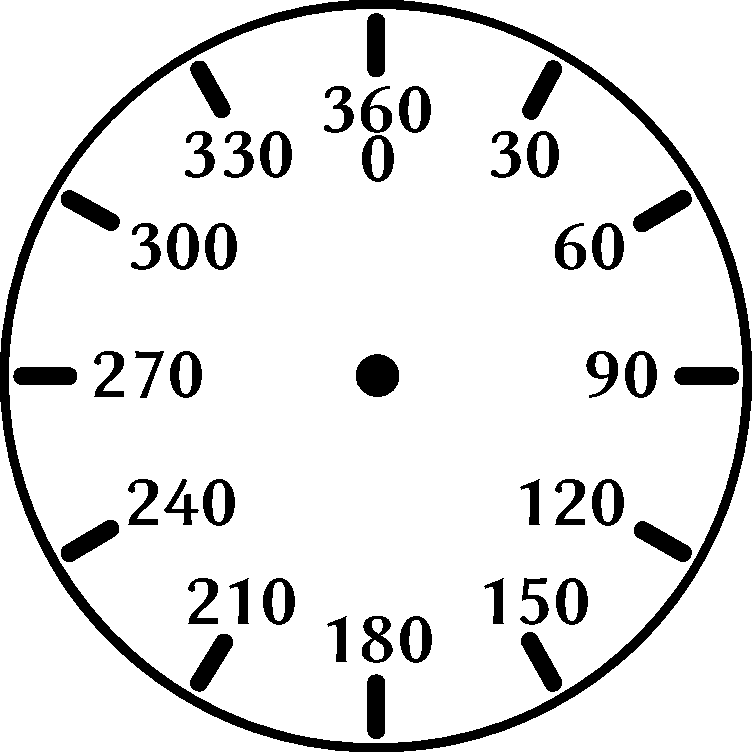
\includegraphics[scale=0.5]{images/degres.pdf}
\caption{Les degrés}
\label{fig:degres}
\end{figure}

Ainsi que veulent vraiment dire «~\texttt{left(90)}~»  ?\\

Si vous êtes debout et face à une direction, pointez un bras directement dans la continuité de votre épaule, voilà c'est 90 degrés de la direction qui vous fait face (c'est un angle droit). Si vous pointez le bras gauche c'est 90 degrés vers la gauche. Si vous pointez le bras droit c'est 90 degrés vers la droite. Quand la tortue Python tourne vers la gauche, elle met son nez sur un point puis pivote son corps pour pointer vers la nouvelle direction (comme si vous aviez tourné votre corps de manière à faire face vers où le bras pointait).\\

Ainsi suite à «~\texttt{tortue.left(90)}~»  la tortue-flèche pointe vers le haut, comme montré dans la figure \ref{fig:90l}.
\begin{figure}[h!]
\centering
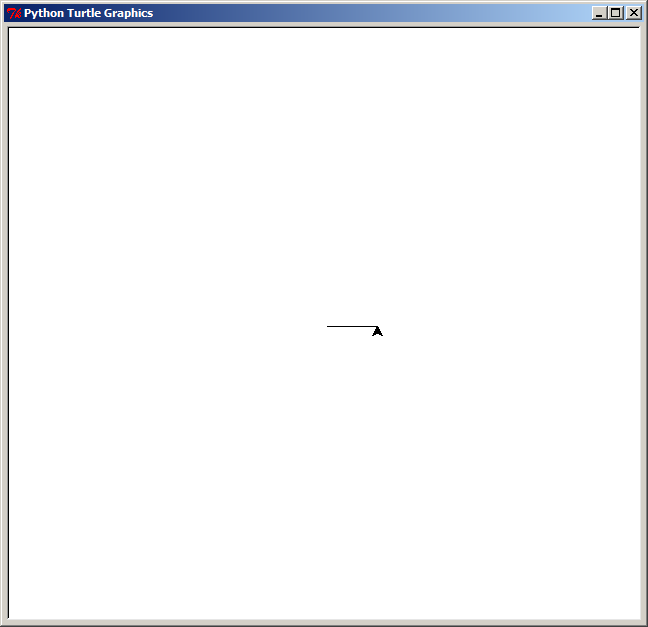
\includegraphics[scale=0.3]{images/90l.png}
\caption{Tortue après avoir tourné de 90°}
\label{fig:90l}
\end{figure}

Recommençons à nouveau quelques fois, en utilisant l'historique:

\begin{Verbatim}[frame=single,rulecolor=\color{mbleu}, label=à taper]
>>> tortue.forward(50)
>>> tortue.left(90)
>>> tortue.forward(50)
>>> tortue.left(90)
>>> tortue.forward(50)
>>> tortue.left(90)
\end{Verbatim}

Notre tortue a dessiné un carré et pointe maintenant dans la même direction et au même endroit que là où elle avait commencé (voir figure \ref{fig:tcar}).
\begin{figure}[h!]
\centering
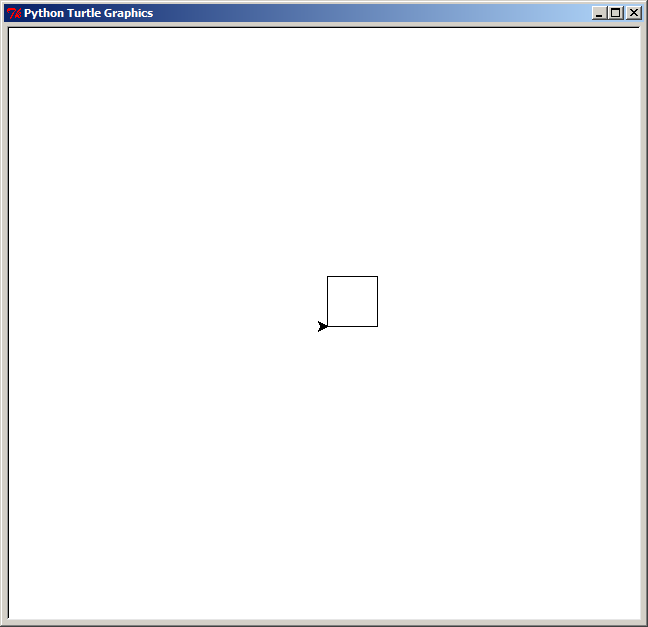
\includegraphics[scale=0.3]{images/tcar.png}
\caption{Tortue après un carré}
\label{fig:tcar}
\end{figure}

Nous pouvons effacer ce qu'il y a sur la zone de dessin en utilisant «~\texttt{clear()}~» (effacer en anglais).

Il  existe quelques autres fonctions que vous pouvez utiliser: 
\begin{itemize}
\item «~\texttt{right()}~»\footnote{droite en anglais} qui tourne la tortue vers la droite;
\item «~\texttt{reset()}~»\footnote{remise à zéro en anglais} qui elle aussi efface l'écran mais replace automatique la tortue à sa position initiale;
\item «~\texttt{backward()}~»\footnote{vers l'arrière en anglais} qui fait reculer la tortue;
\item «~\texttt{up()}~»\footnote{vers le haut} qui dit à la tortue de ne plus dessiner (qui soulève le stylo);
\item «~\texttt{down()}~»\footnote{vers le bas} qui dit à la tortue de dessiner à nouveau.
\end{itemize}
 Vous pouvez utiliser ces fonctions de la même manière que vous avez utilisé les autres:
 
\begin{Verbatim}[frame=single,rulecolor=\color{mbleu}, label=à taper]
>>> tortue.reset()
>>> tortue.backward(100)
>>> tortue.right(90)
>>> tortue.forward(100)
>>> tortue.up()
>>> tortue.forward(100)
>>> tortue.down()
>>> tortue.forward(100)
\end{Verbatim}

Nous reviendrons au module «~\texttt{turtle}~»  bientôt.

\section{À vous de jouer}\label{PRATIQUE:TORTUES}
Dans ce chapitre nous avons vu comment utiliser la tortue pour dessiner de simples lignes, la faire tourner à gauche et à droite. Nous avons vu que la tortue utilise des degrés pour tourner, un peu comme des minutes sur un horloge.

Vous trouverez des pistes de réponses dans la \autoref{REPONSES:TORTUES}.
\subsection*{Exercice 1}
Créez une zone de dessin en utilisant la fonction Pen() de «~\texttt{turtle}~» et dessinez un rectangle.
\subsection*{Exercice 2}
Créez une autre zone de dessin en utilisant la fonction Pen() de «~\texttt{turtle}~» et dessinez un triangle.
 \vfill
\begin{center}
 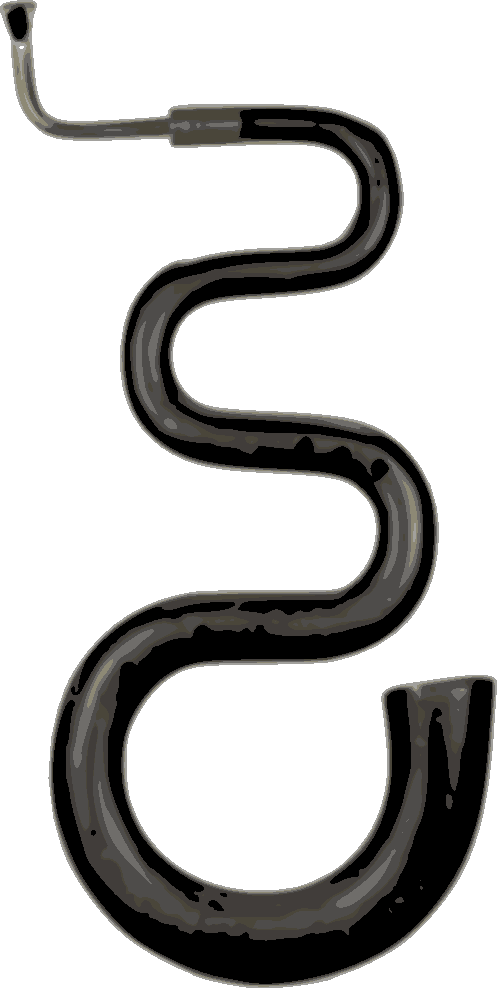
\includegraphics[width=5cm]{images/sem.pdf}
\end{center}
 \vfill

\clearemptydoublepage

% This work is licensed under the Creative Commons Attribution-Share Alike 2.0 France License.
% To view a copy of this license, visit http://creativecommons.org/licenses/by-sa/2.0/fr/legalcode
% or send a letter to Creative Commons, 171 Second Street, Suite 300, San Francisco, California, 94105, USA.


\chapter{Comment poser une question\label{chap:question}}

Attention, l'ensemble des exemples de ce chapitre sont entourés de vert car il faut copier avec exactitude les espaces \emph{ajoutées} dans ces codes. Toutes les indentations de ce chapitre sont composées de quatre espaces (quatre appuis sur la barre d'espace). Ces indentations définissent des blocs que nous verrons dans le chapitre suivant.

Si vous n'entrez pas les espaces correctement vous pourriez avoir une erreur du type:

\begin{Verbatim}[frame=single,rulecolor=\color{red}, label=erreur]
IndentationError: expected an indented block
\end{Verbatim}

\setsansfont[Mapping=tex-text]{DejaVu Sans}
Les espaces et les des tabulations «~\textsf{⇆}~» sont extrêmement importantes en Python. Nous en parlerons en détail dans le chapitre suivant.

\section{Avec des «~si~» on mettrait Paris en bouteille}
En termes de programmation, une question signifie usuellement que nous voulons faire des choses différentes selon 
la réponse à la question. Cela est appelé un «~test si~».

Par exemple:

\emph{Quel âge avez-vous ? Si vous avez plus que 18 ans, vous êtes majeur !}\\


Cela peut être écrit en Python avec le «~\texttt{test si}~» suivant:
\begin{Verbatim}[frame=single,rulecolor=\color{gray}, label=ne pas saisir]
if âge > 18:
    print('Vous êtes majeur !')
\end{Verbatim}

Une représentation graphique peut être observée figure \ref{fig:Cf-if-fr}.

\begin{figure}[ht]
\centering
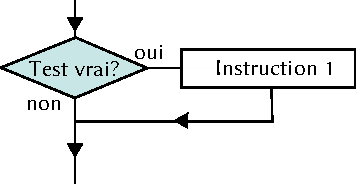
\includegraphics[scale=1.5]{images/Cf-if-fr.pdf}
\caption{Diagramme d'un test «~si~»}
\label{fig:Cf-if-fr}
\end{figure}

Un test \emph{si} est fait d'un «~\texttt{if\footnote{Si l'if est un arbuste en français, il s'agit ici du mot anglais \emph{if} signifie «~si~» en français.}}~» suivi de ce que nous appelons une «~condition~»  (plus de  détails dans une seconde) suivi par deux points «~\verb+:+~». Les lignes qui suivent le «~\texttt{if}~» doivent constituer un bloc; si la réponse à la question est «~oui~» (ou «~vrai~» comme nous le disons en termes de programmation) alors les commandes dans le bloc seront exécutées.\\

Une condition est un élément de programmation qui retourne «~oui~» (vrai) ou «~non~» (faux). Certains symboles (ou opérateurs) sont utilisés pour créer des conditions, comme dans la table \ref{table:opcond}:

\begin{table}[h!]
\begin{center}
\begin{tabular}{|c|c|}
\hline
\texttt{Opérateur}&Opération\\
\hline
\texttt{==}&Égal\\
\hline
\texttt{!=}&Différent\\
\hline
\texttt{>}&Plus grand que\\
\hline
\texttt{<}&Plus petit que\\
\hline
\texttt{>=}&Plus grand ou égal à\\
\hline
\texttt{<=}&Plus petit ou égal à\\
\hline
\end{tabular}
\end{center}
\caption{Opérateurs de condition}
\label{table:opcond}
\end{table}

Par exemple si vous avez 10 ans alors la condition «~\texttt{votre\_âge == 10}~» retournera vrai (oui). Si vous n'avez pas dix ans  elle retournera faux. \\

\fcolorbox{black}{lbleu}{
\centering\begin{minipage}{0.9\textwidth}
Rappelez-vous: ne confondez pas les \emph{deux} symboles utilisés dans une condition «~\texttt{==}~», avec le signe égal utilisé pour assigner une variable. Si vous utiliser un seul symbole «~\texttt{=}~» dans une condition, vous obtiendrez un message d'erreur.\end{minipage}}
\\


Présumons que vous avez attribué votre âge à une variable «~\texttt{âge}~»  et bien si vous avez douze ans la condition «~\texttt{âge > 10}~» sera \emph{vraie}.

Si vous avez huit ans elle retournera \emph{faux}.
Si vous avez dix ans elle retournera \emph{faux} car la condition est vérifiée pour \emph{strictement} plus grand «~\texttt{>}~»  que dix et non pas pour plus grand ou égal «~\texttt{>=}~» à dix.\\

Essayons quelques exemples:

\begin{Verbatim*}[frame=single,rulecolor=\color{green}, label=à taper avec attention]
>>> âge = 10
>>> if âge > 10:
...     print('Arrivé ici !')
\end{Verbatim*}

Si vous avez obtenu une erreur c'est que vous avez oublié quelques espaces (que je vous montre ici en les remplaçant par des @):

\begin{Verbatim}[frame=single,rulecolor=\color{gray}, label=ne pas saisir]
>>> âge = 10
>>> if âge > 10:
... @@@@print('Arrivé ici !')
\end{Verbatim}

Si vous entrez l'exemple ci dessus dans une console qu'arrivera-t-il?\\

\emph{Rien!}\\

Parce que la valeur de la variable «~\texttt{âge}~» n'est pas strictement plus grande que dix, la commande «~\texttt{print}~» dans le bloc ne sera pas lancée. Maintenant étudions:

\begin{Verbatim}[frame=single,rulecolor=\color{green}, label=à taper avec attention]
>>> âge = 10
>>> if âge >= 10:
...     print('Arrivé ici !')
Arrivé ici !
\end{Verbatim}

Si nous essayons cet exemple, alors nous pouvons voir le message affiché. La même chose arrivera avec l'exemple suivant:

\begin{Verbatim}[frame=single,rulecolor=\color{green}, label=à taper avec attention]
>>> âge = 10
>>> if âge == 10:
...     print('Arrivé ici !')
Arrivé ici !
\end{Verbatim}

\begin{center}
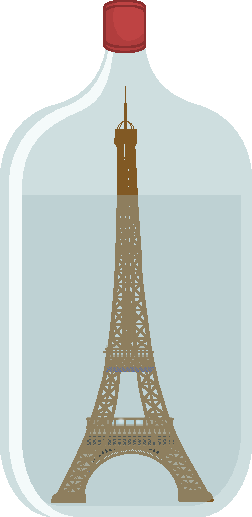
\includegraphics[scale=1]{images/paris.pdf}
\end{center}

\section{Fait cela! Ou sinon...}

Nous pouvons aussi étendre un test «~si~» et faire quelque chose quand la condition n'est pas vraie. Par exemple, afficher le mot «~Bonjour~» sur la console si votre âge est de douze ans mais «~Au revoir~»  s'il est différent. Pour faire cela nous utilisons un test «~si sinon~», ce qui est une autre manière de dire «~si quelque chose est vrai, fais ceci sinon cela~»:

\begin{Verbatim}[frame=single,rulecolor=\color{green}, label=à taper avec attention]
>>> âge = 12
>>> if âge == 12:
...     print('Bonjour !')
... else:
...     print('Au revoir !')
Bonjour !
\end{Verbatim}

Le test «~si sinon~» utilise «~\texttt{if}~» pour si et «~\texttt{else\footnote{Le mot \emph{else} signifie «~sinon~» et provient du latin \emph{alius} (autre) et \emph{alter} (l'autre de deux).}}~» pour sinon.

Rentrez l'exemple ci-dessus et vous devriez voir «~\texttt{Bonjour !}~» affiché dans la console.
Changez la valeur de la variable «~\texttt{âge}~»  à une autre valeur et «~\texttt{Au revoir !}~»  sera affiché:

\begin{Verbatim}[frame=single,rulecolor=\color{green}, label=à taper avec attention]
>>> âge = 8
>>> if âge == 12:
...     print('Bonjour !')
... else:
...     print('Au revoir !')
Au revoir !
\end{Verbatim}

Une représentation graphique peut être observée figure \ref{fig:Cf-else-fr}.

\begin{figure}[ht]
\centering
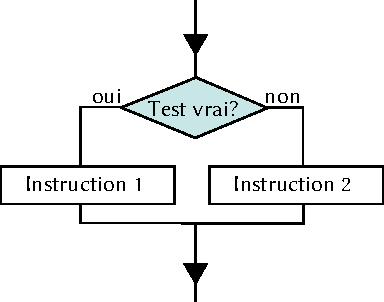
\includegraphics[scale=1.5]{images/Cf-else-fr.pdf}
\caption{Diagramme d'un test «~si~»}
\label{fig:Cf-else-fr}
\end{figure}


\section{Fais cela, ou cela, ou cela! Ou sinon...}
Nous pouvons étendre le test «~si~» encore plus loin en utilisant «~\texttt{elif}~» (l'abréviation  de else-if, «~sinon, si~»). Par exemple, nous pouvons vérifier si votre âge est égal à dix, puis à onze, puis à douze et ainsi de suite: 

\begin{Verbatim}[frame=single,rulecolor=\color{green}, label=à taper avec attention]
>>> âge = 12
>>> if âge == 10:
...     print('Vous avez 10 ans.')
... elif âge == 11:
...     print('Vous avez 11 ans.')
... elif âge == 12:
...     print('Vous avez 12 ans.')
... elif âge == 13:
...     print('Vous avez 13 ans.')
... else:
...     print('Je ne connais pas votre âge.')
Vous avez 12 ans.
\end{Verbatim}

Dans le code ci-dessus, le code vérifie à la deuxième ligne si la valeur de la variable «~\texttt{âge}~» est égale à dix.
Si elle ne l'est pas alors il saute à la quatrième ligne pour vérifier si 
la valeur de la variable «~\texttt{âge}~» est égale à onze. À nouveau  celle-ci     ne l'est pas donc il saute à la sixième ligne  pour vérifier si 
la valeur de la variable «~\texttt{âge}~» est égale à douze. Dans ce cas cela est le cas donc Python va dans le bloc à la septième ligne et exécute la commande «~\texttt{print}~».
Vous avez probablement remarqué qu'il a cinq groupes dans ce code aux lignes 3, 5, 7, 9 et 11.

Une représentation graphique peut être observée figure \ref{fig:Cf-elif-fr}.

\begin{figure}[ht]
\centering
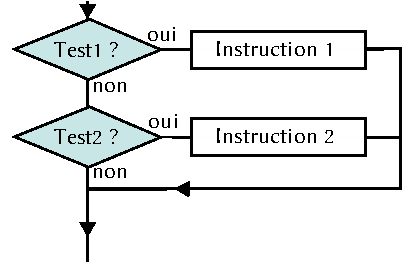
\includegraphics[scale=1.5]{images/Cf-elif-fr.pdf}
\caption{Diagramme d'un test «~si~»}
\label{fig:Cf-elif-fr}
\end{figure}

\section{Combiner des conditions}
Vous pouvez combiner des conditions ensemble en utilisant les mots clef «~\texttt{and}~» qui signifie «~et~» et «~\texttt{or}~» qui signifie «~ou~».

Nous pouvons condenser l'exemple précédent, un petit peu, en utilisant «~\texttt{or}~» pour joindre les conditions ensemble:

\begin{Verbatim}[frame=single,rulecolor=\color{green}, label=à taper avec attention]
>>> if âge == 10 or âge == 11 or âge == 12 or âge == 13:
...     print('Vous avez %s ans.' % âge)
... else:
...     print('Heu ?')
\end{Verbatim}

Si n'importe laquelle des conditions de la première ligne est vraie, c'est à dire si  «~\texttt{âge}~» est égal à 10, 11, 12 ou 13, alors le bloc de code ligne 2 sera exécuté. Sinon Python ira à la quatrième ligne. 
Nous pouvons condenser ce code un peu plus en utilisant les opérateurs «~\texttt{and}~», «~\texttt{>=}~», «~\texttt{<=}~»:

\begin{Verbatim}[frame=single,rulecolor=\color{green}, label=à taper avec attention]
>>> if âge >= 10 and âge <= 13:
...     print('Vous avez %s ans.' % âge)
... else:
...     print('Heu ?')
\end{Verbatim}

Vous avez probablement compris que si les deux conditions de la première ligne sont vraies alors le bloc de la deuxième ligne est exécuté (si «~\texttt{âge}~»  est plus grand ou égal à dix et «~\texttt{âge}~» est plus petit ou égal à 13. Donc si la variable «~\texttt{âge}~» vaut douze alors «~\texttt{Vous avez 12 ans.}~» sera affiché sur la console parce que douze est plus grand que dix et plus petit que treize.

\section{Rien}
Il y a une autre sorte de valeur qui peut être assignée à une variable et dont nous n'avons pas encore parlé dans les chapitres précédents: \textbf{rien}!

De la même manière que les nombres, les chaînes et les listes peuvent être assignés à des variables, «~{rien}~»  est aussi un type de valeur qui peut être assigné. En Python une valeur vide est désignée comme «~\texttt{None\footnote{Le mot \emph{none} signifie aucun, personne en anglais, contraction de \emph{no one} pas un.}}~».

Une variable valant «~\texttt{None}~» (dans d'autres langages, «~\texttt{null}~» est parfois utilisé) peut être utilisée comme les autres variables:

\begin{Verbatim}[frame=single,rulecolor=\color{mbleu}, label=à taper]
>>> maval = None
>>> print(maval)
None
\end{Verbatim}

\begin{center}
\textcolor{blue}{\textrm{\scalefont{5}\{\}==∅==None}}
\end{center}

«~\texttt{None}~» est une manière de réinitialiser une variable comme étant non utilisée ou une manière de créer une variable sans fixer sa valeur avant de l'utiliser.

Par exemple si votre équipe de football lève des fonds pour de nouveaux uniformes, vous voulez peut-être attendre que toute l'équipe soit revenue avec l'argent récolté, avant d'ad\-di\-tion\-ner les montants. En termes de programmation, vous pouvez avoir une variable pour chaque joueur de l'équipe et initialiser ces variables à «~\texttt{None}~»:

\begin{Verbatim}[frame=single,rulecolor=\color{mbleu}, label=à taper]
>>> joueur1 = None
>>> joueur2 = None
>>> joueur2 = None
\end{Verbatim}

Nous pouvons utiliser un test «~si~» pour vérifier ces variables de manière à déterminer si tous les membres de l'équipe sont revenus avec l'argent qu'ils ont levé:

\begin{Verbatim}[frame=single,rulecolor=\color{green}, label=à taper avec attention]
>>> if joueur1 is None or joueur2 is None or joueur3 is None:
...     print('''S'il-vous-plait, attendez jusqu'à ce 
...que tous les joueurs soient revenus.''')
... else:
...     print('Vous avez levé %s€' % (player1 + player2 + player3))
\end{Verbatim}

Le test «~si~» contrôle si une des variables a une valeur nulle et affiche le premier message si cela est la cas.

Le mot \emph{is} est la troisième personne du verbe \emph{to be}, c'est à dire «~être~» en français. Le test est donc «~Est ce que joueur1, joueur2 ou joueur3 sont nuls?~». 

Si chaque variable a une valeur non nulle alors le second message est affiché avec la somme totale récoltée.
Si vous essayez le code avec toutes les variables qui pointent vers «~\texttt{None}~»,  vous aurez le premier message (n'oubliez pas de créer les variables d'abord ou vous aurez un message d'erreur):

\begin{Verbatim}[frame=single,rulecolor=\color{green}, label=à taper avec attention]
>>> if joueur1 is None or joueur2 is None or joueur3 is None:
...     print('''S'il-vous-plait, attendez jusqu'à ce 
...que tous les joueurs soient revenus.''')
... else:
...     print('Vous avez levé %s€' % (player1 + player2 + player3))
S'il-vous-plait, attendez jusqu'à ce 
que tous les joueurs soient revenus.
\end{Verbatim}

Même si vous avez modifié une ou deux variables, vous continuerez d'avoir le même message:

\begin{Verbatim}[frame=single,rulecolor=\color{green}, label=à taper avec attention]
>>> joueur1=100
>>> joueur2=300
>>> if joueur1 is None or joueur2 is None or joueur3 is None:
...     print('''S'il-vous-plait, attendez jusqu'à ce 
...que tous les joueurs soient revenus.''')
... else:
...     print('Vous avez levé %s€' % (player1 + player2 + player3))
S'il-vous-plait, attendez jusqu'à ce 
...que tous les joueurs soient revenus.
\end{Verbatim}

Finalement une fois toutes les variables modifiées vous verrez le message du second bloc:

\begin{Verbatim}[frame=single,rulecolor=\color{green}, label=à taper avec attention]
>>> joueur1=100
>>> joueur2=300
>>> joueur3=400
>>> if joueur1 is None or joueur2 is None or joueur3 is None:
...     print('''S'il-vous-plait, attendez jusqu'à ce 
...que tous les joueurs soient revenus.''')
... else:
...     print('Vous avez levé %s€' % (player1 + player2 + player3))
Vous avez levé 800€
\end{Verbatim}

\section{Quelle est la différence?\label{sec:dif}}

Quelle est la différence entre «~\texttt{«~10~»}~» et «~\texttt{'10'}~»?
Pas grande mis à part les apostrophes, pouvez-vous penser. Et bien, si vous avez bien lu les chapitres précédents vous savez que le premier est un nombre et que le second est une chaîne. Cela les rend plus différents que ce à quoi vous pourriez vous attendre. Auparavant nous avions comparé la valeur de la variable «~\texttt{âge}~» à un nombre dans un test «~si~»:

\begin{Verbatim}[frame=single,rulecolor=\color{green}, label=à taper avec attention]
>>> if âge == 10:
...     print('Vous avez 10 ans.')
\end{Verbatim}

Si vous aviez attribué dix à la variable «~\texttt{âge}~»  la fonction «~\texttt{print}~»  sera appelée:

\begin{Verbatim}[frame=single,rulecolor=\color{green}, label=à taper avec attention]
>>> âge = 10
>>> if âge == 10:
...     print('Vous avez 10 ans.')
...
Vous avez 10 ans.
\end{Verbatim}

Mais si «~\texttt{âge}~»  a pour valeur «~\texttt{"10"}~» alors la fonction «~\texttt{print}~» ne sera pas appelée:

\begin{Verbatim}[frame=single,rulecolor=\color{green}, label=à taper avec attention]
>>> âge = '10'
>>> if âge == 10:
...     print('Vous avez 10 ans.')
...
\end{Verbatim}

Pourquoi le code dans le bloc n'a pas été exécuté? Parce qu'une chaîne est différente d'un nombre, même s'ils se ressemblent:

\begin{Verbatim}[frame=single,rulecolor=\color{mbleu}, label=à taper]
>>> âge1 = 10
>>> âge2 = '10'
>>> print(âge1)
10
>>> print(âge2)
10
\end{Verbatim}

Regardez! Ils semblent exactement identiques. Pourtant, parce que l'un est une chaîne et l'autre est un nombre, ils ont des valeurs différentes. Néanmoins après «~\texttt{âge="10"}~», «~\texttt{âge == 10}~»  sera toujours faux tant qu'«~\texttt{âge}~» sera une chaîne.  Nous sommes trompés par Python dont la fonction «~\texttt{print}~» est capable de convertir un nombre en chaîne pour l'afficher.

Il y a probablement une meilleure manière de penser les choses: c'est de considérer dix livres et dix briques. Le nombre d'éléments peut être le même mais vous ne diriez pas que dix livres sont exactement la même chose que dix briques, n'est-ce-pas? Par chance, en Python nous avons des fonctions magiques qui peuvent transformer des chaînes en nombres et des nombres en chaînes même si elles ne peuvent pas vraiment transformer les briques en livres. Par exemple, pour convertir la chaine «~\texttt{'10'}~»  en un nombre vous pouvez utiliser la fonction «~\texttt{int}~»: 

\begin{Verbatim}[frame=single,rulecolor=\color{mbleu}, label=à taper]
>>> âge_en_chaîne = '10'
>>> âge_en_nombre = int(âge)
>>> print(âge_en_chaîne*2)
1010
>>> print(âge_en_nombre*2)
20
\end{Verbatim}

L'abbreviation «~\texttt{int}~»  est utilisé  pour \emph{integer} qui signifie entier en anglais. C'est-à-dire un nombre entier (sans virgule).\\

La variable «~\texttt{âge\_en\_nombre}~» contient le nombre dix et pas une chaîne. Pour convertir un nombre en une chaîne, vous pouvez utiliser la fonction «~\texttt{str}~»:


\begin{Verbatim}[frame=single,rulecolor=\color{mbleu}, label=à taper]
>>> âge_en_nombre = 10
>>> âge_en_chaîne = str(âge_en_nombre)
\end{Verbatim}

L'abréviation «~\texttt{str}~» est utilisée au lieu de \emph{string} qui signifie ficelle en anglais mais plus particulièrement chaîne de caractères en programmation\footnote{L'appellation française est pour une fois nettement plus compréhensible que la forme originale en anglais.}.\\

«~\texttt{âge\_en\_chaîne}~» contient la chaîne «~\texttt{'10'}~» et non pas un nombre. Revenons à notre test «~si~» qui n'imprimait rien:

\begin{Verbatim}[frame=single,rulecolor=\color{green}, label=à taper avec attention]
>>> âge = '10'
>>> if âge == 10:
...     print('Vous avez dix ans.')
...
\end{Verbatim}

Si nous convertissons la variable avant le test alors nous aurons un résultat différent:

\begin{Verbatim}[frame=single,rulecolor=\color{green}, label=à taper avec attention]
>>> âge = '10'
>>> âge_converti=int(âge)
>>> if âge_converti == 10:
...     print('Vous avez dix ans.')
...
Vous avez dix ans.
\end{Verbatim}

\vfill
\begin{center}
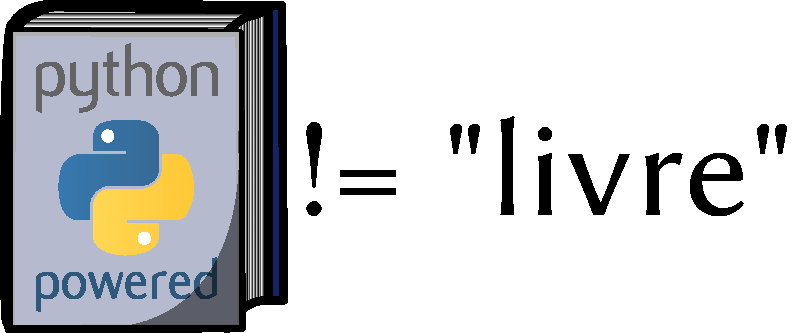
\includegraphics[scale=1]{images/livre.pdf} 
\end{center}
\vfill

\clearemptydoublepage

% This work is licensed under the Creative Commons Attribution-Share Alike 2.0 France License.
% To view a copy of this license, visit http://creativecommons.org/licenses/by-sa/2.0/fr/legalcode
% or send a letter to Creative Commons, 171 Second Street, Suite 300, San Francisco, California, 94105, USA.



\chapter{Encore et encore}
\section{Rabâchage}
Il n'y pas grand chose de pire que de faire la même chose encore et encore\footnote{\url{http://fr.wikipedia.org/wiki/Sisyphe}}.
C'est la raison pour laquelle vos parents vous disent de compter les moutons pour essayer de dormir et cela n'a rien avoir avec les incroyables pouvoirs somnifères des mammifères laineux. Cela  a tout avoir avec le fait que répéter quelque chose sans fin est ennuyeux, et que votre esprit devrait tomber dans le sommeil plus facilement s'il n'est pas en train de se concentrer sur quelque chose d'intéressant.\\


Les programmeurs, eux aussi, n'aiment pas particulièrement répéter les choses. Cela les endort aussi. C'est la vraie raison pour laquelle tous les langages de programmation de haut niveau\footnote{Les boucles ont été introduites avec le langage Fortran en 1958.} ont quelque chose appelé une boucle. Par exemple pour afficher «~hello~»  cinq fois en Python vous pouvez faire comme suit:

\begin{Verbatim}[frame=single,rulecolor=\color{gray}, label=ne pas saisir]
>>> print("hello")
hello
>>> print("hello")
hello
>>> print("hello")
hello
>>> print("hello")
hello
>>> print("hello")
hello
\end{Verbatim}

\emph{Ce qui est... Plutôt ennuyant, pour être poli.}\\


Ou nous pouvons utiliser une boucle:

\begin{Verbatim}[frame=single,rulecolor=\color{green}, label=à taper avec attention]
>>> for x in range(0, 5):
...     print('hello')
...
hello
hello
hello
hello
hello
\end{Verbatim}

Comme au chapitre précédent les espaces sont importants, je vous les montre de manière plus explicite avec des arobases:

\begin{Verbatim}[frame=single,rulecolor=\color{gray}, label=ne pas saisir]
>>> for x in range(0, 5):
... @@@@print('hello')
...
\end{Verbatim}

Le mot \emph{for} signifie «~pour~»  en anglais, \emph{in} signifie «~dans~» et \emph{range} signifie gamme (de produit), éventail (de valeurs), série (de valeurs).

La fonction «~\texttt{range}~» permet de créer facilement et rapidement une liste (une série) de nombre entre un début et une fin, par exemple:

\begin{Verbatim}[frame=single,rulecolor=\color{mbleu}, label=à taper]
>>> print(list(range(10, 20)))
[10, 11, 12, 13, 14, 15, 16, 17, 18, 19]
\end{Verbatim}

Si nous ne fournissons qu'un nombre à «~\texttt{range}~» la liste part de zéro («~\texttt{range(n) == range(0,n)}~»:

\begin{Verbatim}[frame=single,rulecolor=\color{mbleu}, label=à taper]
>>> print(list(range(5)))
[0, 1, 2, 3, 4]
\end{Verbatim}

Le mot \emph{list} signifie liste (oui je sais vous aviez deviné).

Dans le cas de Python la boucle utilisée s'appelle un itérateur. Le code «~\texttt{for x in range(0,5)}~» dit en fait à Python de créer une liste de nombre (0, 1, 2, 3, 4) puis pour chacun de ces nombres de stocker cette valeur dans la variable «~\texttt{x}~» et enfin d'exécuter la commande dans le bloc après les deux points pour chaque valeur de «~\texttt{x}~». Nous pouvons utiliser ce «~\texttt{x}~»  dans notre déclaration qui contient «~\texttt{print}~» si nous le voulons:

\begin{Verbatim}[frame=single,rulecolor=\color{green}, label=à taper avec attention]
>>> for x in range(0, 5):
...     print('hello %s' % x)
hello 0
hello 1
hello 2
hello 3
hello 4
\end{Verbatim}

Une représentation graphique peut être observée figure \ref{fig:for}.
\begin{figure}[ht]
\centering
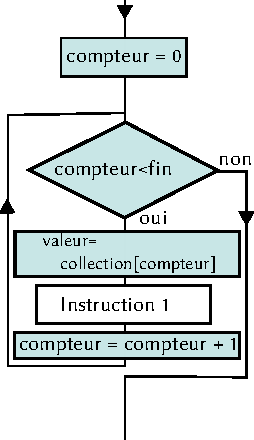
\includegraphics[scale=1.5]{images/for.pdf}
\caption{Diagramme d'un itérateur}
\label{fig:for}
\end{figure}

Si nous déroulions la boucle que nous venons d'éxécuter, cela pourrait ressembler à quelque chose comme cela:

\begin{Verbatim}[frame=single,rulecolor=\color{gray}, label=ne pas saisir]
x = 0
print('hello %s' % x)
x = 1
print('hello %s' % x)
x = 2
print('hello %s' % x)
x = 3
print('hello %s' % x)
x = 4
print('hello %s' % x)
\end{Verbatim}

Ainsi cette boucle (cet itérateur) nous a épargné d'écrire huit lignes de code supplémentaires. C'est vraiment utile, d'autant plus que le programmeur moyen est plus encore paresseux qu'un hippopotame (un jour chaud) quand il s'agit de taper quelque chose. Les bons programmeurs détestent faire les choses plus d'une fois, donc les boucles sont une des structures les plus utiles dans un langage de programmation.\\

Nous n'avons pas obligation d'utiliser «~\texttt{range}~», nous pouvons utiliser les listes que nous avons déjà utilisées:

\begin{small}
\begin{Verbatim}[frame=single,rulecolor=\color{green}, label=à taper avec attention]
>>> courses=['lait', 'fromage', 'laitue', 'confiture', 'sirop', 'chocolat']
>>> for i in courses:
...     print(i)
lait
fromage
laitue
confiture
sirop
chocolat
\end{Verbatim}
\end{small}

Le code si dessus est une manière de dire: «~pour chaque élément de la liste, stocke la valeur dans la variable \texttt{i} et affiche le contenu de cette variable~»\footnote{Les variables utilisées dans les boucles simples ont rarement des noms explicites. Dans une boucle plus complexe «~\texttt{produit\_à\_acheter}~» pourrait être plus opportun.}.  À nouveau si nous déroulons la boucle nous aurons quelque chose comme:

\begin{small}
\begin{Verbatim}[frame=single,rulecolor=\color{gray}, label=ne pas saisir]
>>> courses=['lait', 'fromage', 'laitue', 'confiture', 'sirop', 'chocolat']
>>> print(courses[0])
lait
>>> print(courses[1])
fromage
>>> print(courses[2])
laitue
>>> print(courses[3])
confiture
>>> print(courses[4])
sirop
>>> print(courses[5])
chocolat
\end{Verbatim}
\end{small}

De nouveau la boucle nous a épargné beaucoup d'écriture.

\begin{center}
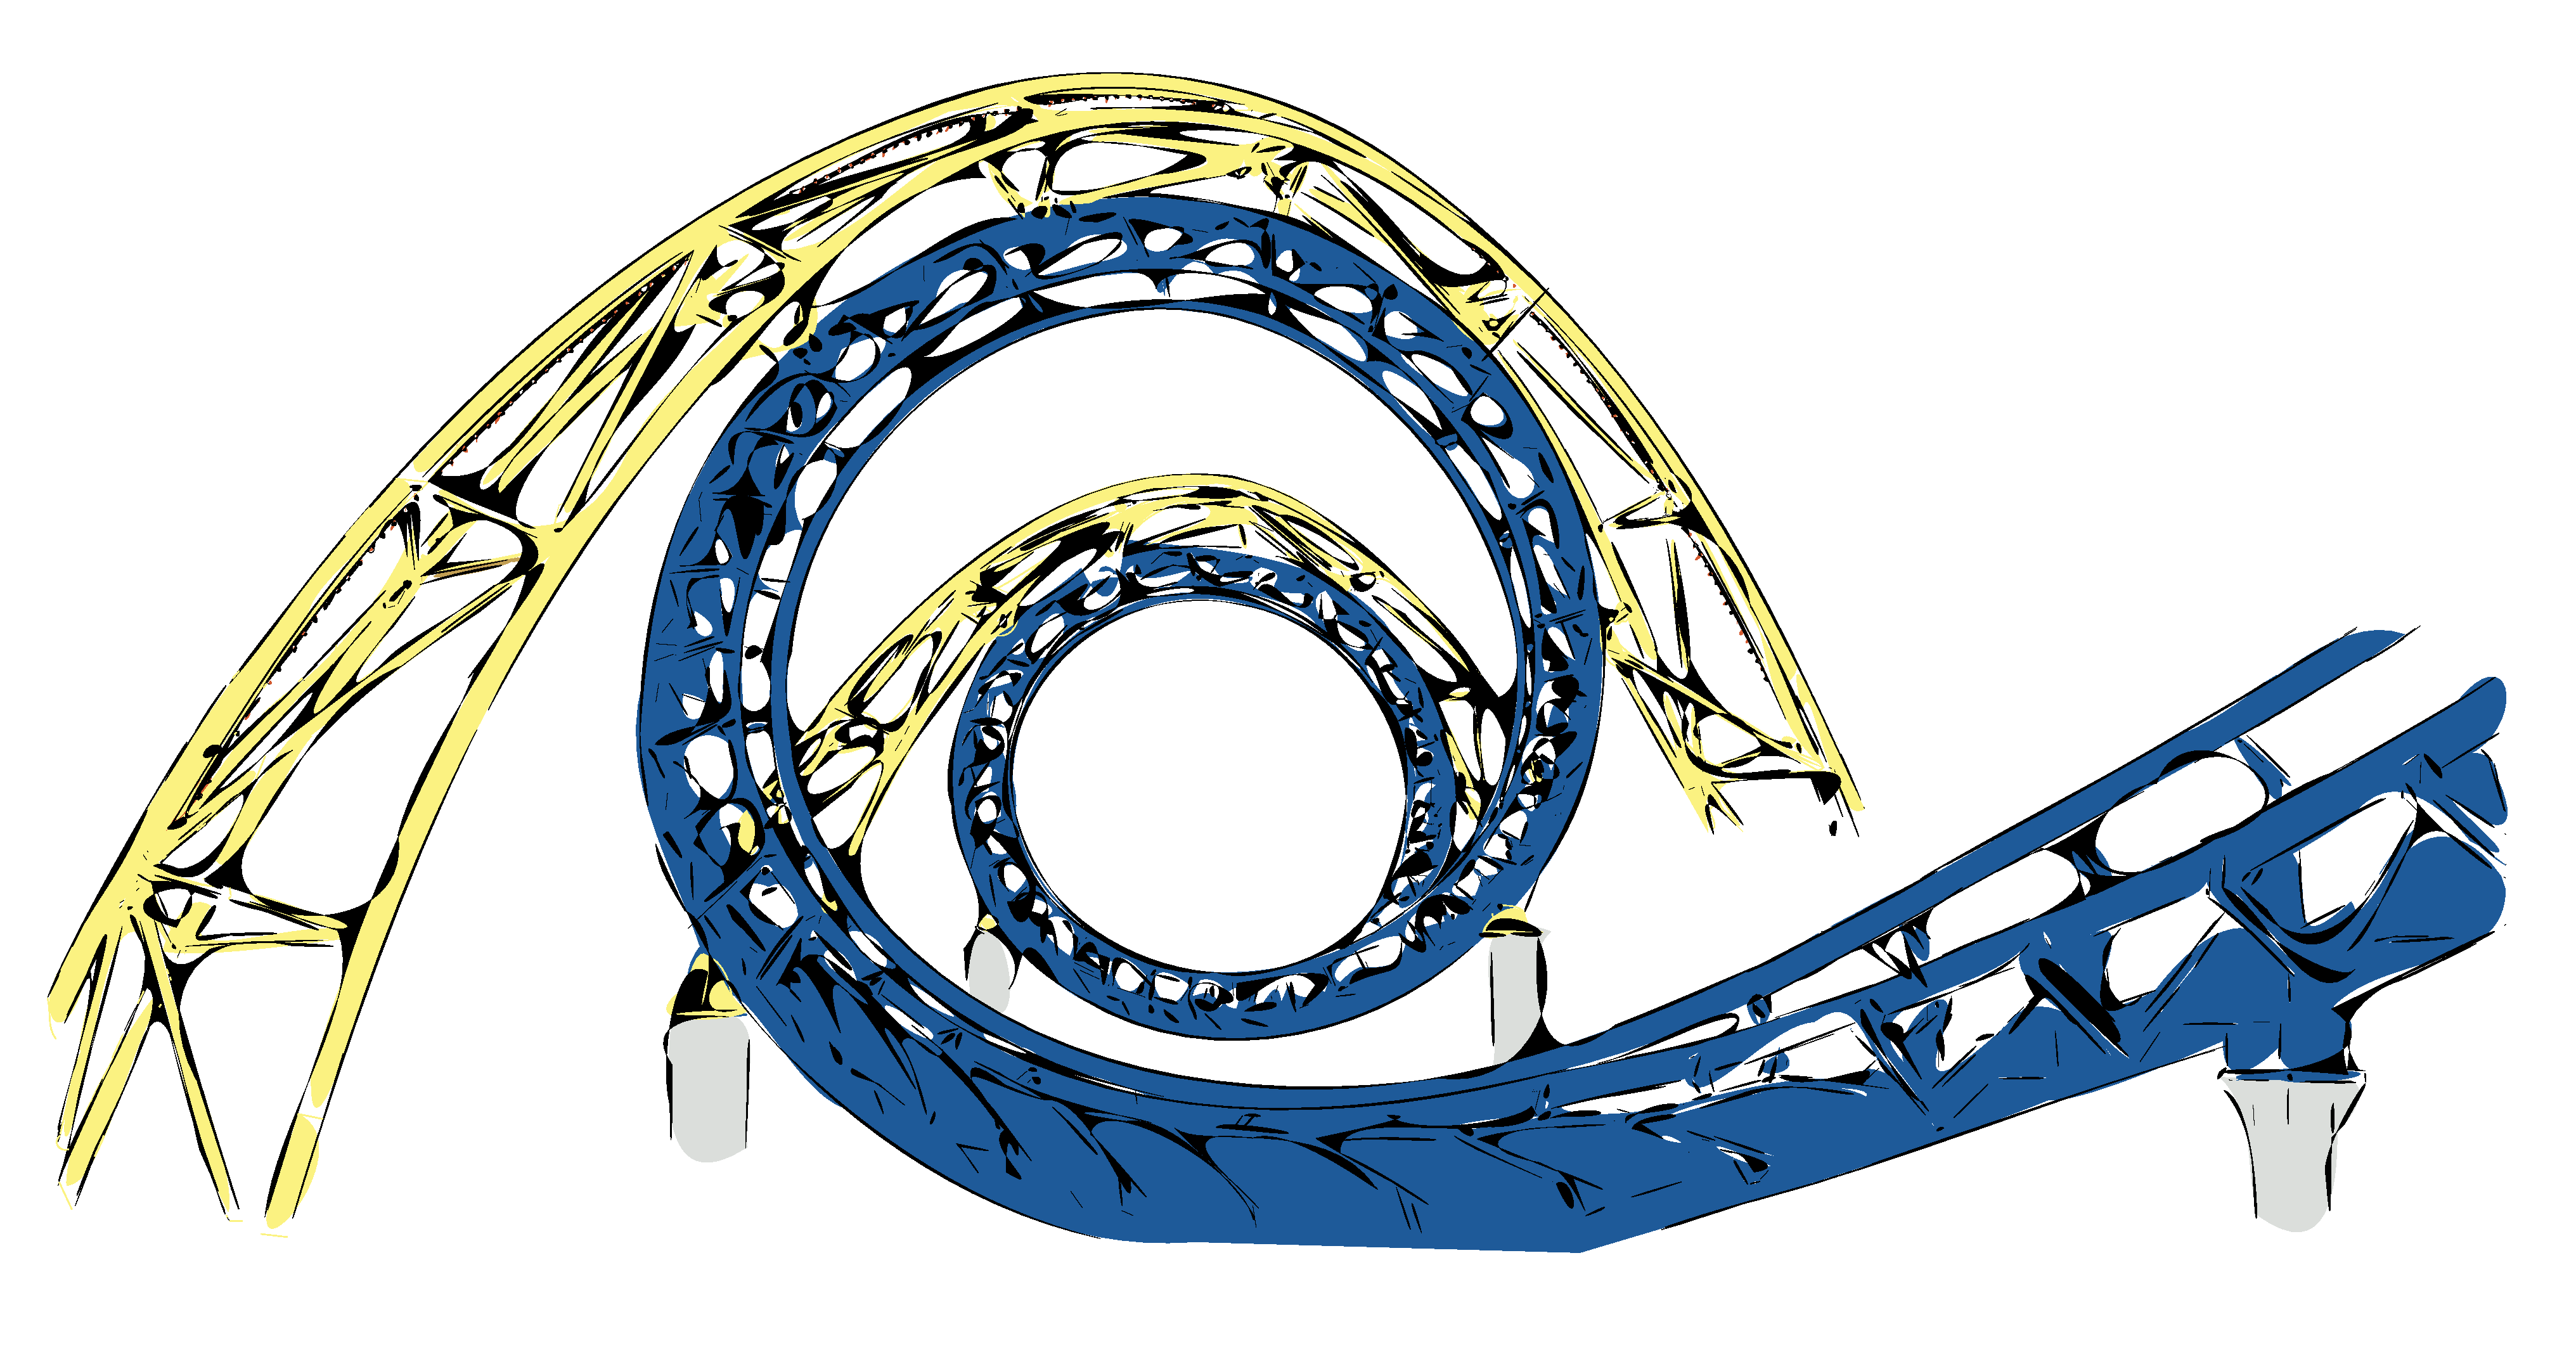
\includegraphics[scale=.2]{images/SteveLambert_Roller_Coaster_Tracks.pdf} 
\end{center}


\section{Quand est-ce qu'un bloc n'est pas compact?}
Quand c'est un bloc de code.\\

Qu'est-ce qu'un «~bloc de code~», alors?\\

Un bloc de code est une série d'instructions que vous voulez grouper ensemble.
Par exemple, dans la boucle ci-dessus vous pourriez avoir envie de faire plus qu'afficher des éléments. 
Peut-être que vous voudriez acheter chaque objet et afficher qu'il l'a bien été.
Supposons que nous avons une fonction appelé «~\texttt{acheter}~» vous pourriez écrire quelque chose comme cela :

\begin{Verbatim}[frame=single,rulecolor=\color{gray}, label=ne pas saisir]
>>> for i in courses :
... 	acheter(i)
... 	print(i)
\end{Verbatim}

Ne vous cassez pas la tête à taper cet exemple dans la console Python car nous n'avons pas de fonction «~\texttt{acheter}~» et que vous auriez un message d'erreur si vous tentiez de la lancer. 
Néanmoins cet exemple permet de montrer un bloc fait de deux commandes:

\begin{Verbatim}[frame=single,rulecolor=\color{gray}, label=ne pas saisir]
acheter(i)
print(i)
\end{Verbatim}

De manière plus utile nous pouvons aussi tracer un cercle avec la tortue sans fonction cercle:

\begin{Verbatim}[frame=single,rulecolor=\color{green}, label=à taper avec attention]
>>> import turtle
>>> tortue=turtle.Pen()
>>> for i in range(360):
...     tortue.forward(1)
...     tortue.left(1)
...
\end{Verbatim}

Vous pouvez observer le résultat sur la figure \ref{fig:cercle}.
\begin{figure}[H]
\centering
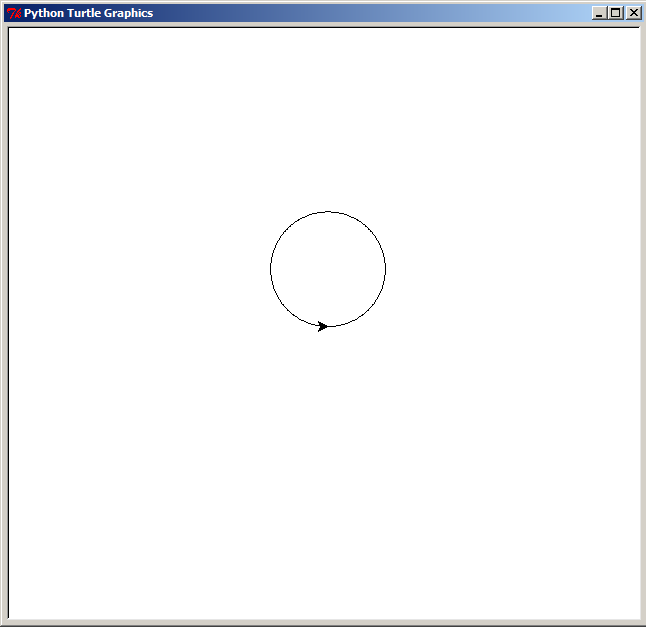
\includegraphics[scale=0.4]{images/cercle.png}
\caption{Un cercle fait en 360 étapes}
\label{fig:cercle}
\end{figure}


En Python, les espaces que ce soient des espaces normales ou des tabulations «~\textsf{⇆}~» sont extrêmement  importantes (bis). Le code qui est positionné à la même position horizontalement est groupé ensemble en blocs.\\


La figure \ref{fig:blocs} montre le découpage en bloc selon la position.
\begin{figure}[H]
\centering
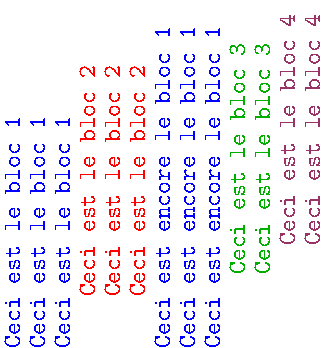
\includegraphics[scale=1,angle=270]{images/blocs.pdf}
\caption{Les blocs en Python}
\label{fig:blocs}
\end{figure}

On commence un nouveau bloc après une ligne finissant   par «~\verb+:+~». Le nouveau bloc est défini par rapport à son indentation (la distance avec le bord gauche). Le bloc initié par «~\verb+:+~» doit avoir une indentation plus grande (être plus à droite) que le bloc précédent.\\


Attention vous devez être cohérents avec vos espacements. Par exemple, nous aurons une erreur avec:

\begin{Verbatim}[frame=single,rulecolor=\color{red}, label=erreur]
>>> for i in courses:
...     acheter(i)
...       print(i)
\end{Verbatim}

La seconde ligne (avec la fonction «~\texttt{acheter(i)}~») commence avec \textbf{quatre} espaces. La troisième ligne commence avec \textbf{six} espaces. Regardons attentivement le code en mettant en valeur les espaces avec des arobases:

\begin{Verbatim}[frame=single,rulecolor=\color{gray}, label=ne pas saisir]
>>> for i in courses:
... @@@@acheter(i)
... @@@@@@print(i)
\end{Verbatim}

Cela causera une erreur. Quand nous commençons un bloc avec quatre espaces vous devez continuer quatre espaces. Et cela tant que vous ne créez pas un nouveau bloc avec «~\verb+:+~» ou que vous ne finissiez pas le bloc en revenant à un niveau d'indentation précédent.\\

Il est d'usage d'indenter les blocs avec des espaces, ou pour le moins, de ne pas mélanger les espaces et les tabulations. De plus on utilise généralement des pas d'indentation constant de quatre espaces.
Si vous commencez un bloc dans un bloc indenté de quatre espaces, il convient d'indenter le nouveau de huit (2x4).
Par exemple, on tapera:

\begin{Verbatim}[frame=single,rulecolor=\color{gray}, label=ne pas saisir]
@@@@un premier bloc
@@@@un premier bloc
@@@@un premier bloc
@@@@@@@@un deuxième bloc
@@@@@@@@un deuxième bloc
@@@@@@@@un deuxième bloc
\end{Verbatim}

Pourquoi allons nous vouloir mettre un bloc «~dans~» un autre? Généralement nous faisons cela quand le deuxième bloc repose sur le premier d'une certaine façon, comme dans une boucle.

Si nous commençons une boucle dans le premier bloc alors les instructions que nous voulons exécuter encore et encore sont dans le second, le second bloc repose sur le premier pour fonctionner correctement.\\

Dans une console Python, une fois que vous commencez à taper du code dans un bloc, Python continue ce bloc jusqu'à ce que vous pressiez entrée sur une ligne vide (ou que vous changez de bloc). Vous pouvez observer trois points au début de chaque ligne qui indiquent que vous continuez à être dans un bloc.\\

Essayons maintenant quelques \emph{vrais} exemples. Ouvrez la console et tapez ce qui suit en vous rappelant de presser la barre d'espace quatre fois au début des lignes qui commencent par «~\texttt{print}~»:

\begin{Verbatim}[frame=single,rulecolor=\color{green}, label=à saisir avec attention]
>>> maliste = [ 'a', 'b', 'c' ]
>>> for i in maliste:
...     print(i)
...     print(i)
...
a
a
b
b
c
c
\end{Verbatim} 

Après le second «~\texttt{print}~» appuyez sur la touche entrée sur la ligne blanche pour dire à la console que vous souhaitez finir le bloc. Cela affichera chaque élément deux fois.\\

L'exemple suivant va créer un message d'erreur:

\begin{Verbatim}[frame=single,rulecolor=\color{red}, label=erreur]
>>> maliste = [ 'a', 'b', 'c' ]
>>> for i in maliste:
...     print(i)
...       print(i)
...
File <stdin>, line 3
print(i)
^
IndentationError: unexpected indent
\end{Verbatim}

La seconde ligne avec «~\texttt{print}~» a six espaces et non quatre sans avoir été introduite par deux points. Python n'aime pas cela car l'indentation doit rester la même au sein d'un même bloc.

\begin{center}

\fcolorbox{black}{lbleu}{
 \begin{minipage}{12cm}
\textbf{Pense-bête}\\

Si vous commencez un bloc de code avec quatre espaces vous devez continuer avec quatres espace. De plus il est conseillé de toujours utiliser des indentations multiples de la première indentation choisie comme 4, 8, 12.

La pluspart des programmeurs Python utilisent des indentations de quatres espaces. Pour faciliter l'éventuelle fusion de code, il est donc conseillé d'utiliser, vous aussi des indentations de quatres espaces.

De plus si vous utilisez IDLE comme éditeur (pas dans le Shell) l'appui sur la touche tabulation «~\textsf{⇆}~» insérera quatres espaces. Le shell IDLE ajoute automatiquement une indentation réalisée avec une tabulation. Le passage d'un bloc à un autre sur une ligne peut être fait en utilisant les flèches horizontales.

\end{minipage}
 }
\end{center}



Vois un exemple qui met en œuvre deux blocs de code:

\begin{Verbatim}[frame=single,rulecolor=\color{gray}, label=ne pas saisir]
>>> maliste = [ 'a', 'b', 'c' ]
>>> for i in maliste:
...     print(i)
...     for j in maliste:
...         print(j)
...
\end{Verbatim}

Où sont les blocs dans ce code que va-t-il faire?
Il a deux blocs, le premier fait parti de la première boucle:

\begin{Verbatim}[frame=single,rulecolor=\color{gray}, label=ne pas saisir]
>>> maliste = [ 'a', 'b', 'c' ]
>>> for i in maliste:
...     print(i)              # Ces deux lignes sont
...     for j in maliste:     # le premier bloc
...         print(j)
...
\end{Verbatim}

Le deuxième bloc est la ligne «~\texttt{print}~» solitaire dans la seconde boucle:

\begin{Verbatim}[frame=single,rulecolor=\color{gray}, label=ne pas saisir]
>>> maliste = [ 'a', 'b', 'c' ]
>>> for i in maliste:
...     print(i) 
...     for j in maliste:
...         print(j)          # Second bloc
...
\end{Verbatim}

Au passage vous pouvez observer des dièses «~\texttt{\#}~» qui sont utilisés pour marquer des commentaires. Les commentaires sont du texte qui n'est pas pris en compte pour l'éxécution mais qui apporte des informations sur le code et permettent de le documenter (pour un usage ultérieur par exemple).\\


Pouvez-vous déduire ce que ce petit bout de code va faire?
Il va afficher les trois lettres de «~\texttt{maliste}~», mais combien de fois?
Si nous étudions chaque ligne nous pouvons probablement trouvez ce nombre de fois.
Nous savons que la première boucle va parcourir tous les objets de la liste et exécuter
les commandes du premier bloc. Donc elle va afficher une lettre puis lancer la seconde boucle. Cette boucle va elle aussi parcourir les éléments de la liste et exécuter les commandes du deuxième bloc. Ainsi nous pouvons comprendre ce qui est affiché quand le code est exécuté, ce sera un «~\texttt{a}~»  suivi de «~\texttt{a}~», «~\texttt{b}~», «~\texttt{c}~» puis un «~\texttt{b}~»  suivi de «~\texttt{a}~», «~\texttt{b}~», «~\texttt{c}~» et ainsi de suite.\\

Entre le code dans console et voyez par vous-même:

\begin{Verbatim}[frame=single,rulecolor=\color{green}, label=à saisir avec attention]
>>> maliste = [ 'a', 'b', 'c' ]
>>> for i in maliste:
...     print(i)
...     for j in maliste:
...         print(j)
...
a
a
b
c
b
a
b
c
c
a
b
c
\end{Verbatim}

Et si nous faisions maintenant quelque chose de plus utile que juste afficher des lettres?
Rappelez-vous les calculs que nous avions fait au début de ce livre sur les économies que vous pourriez réaliser. Il s'agissait de calculer les économies si vous gagniez 10\begin{small}\euro\end{small} par semaine en faisant le ménage, 30\begin{small}\euro\end{small} en distribuant le journal et vous dépensiez 10\begin{small}\euro\end{small}.\\

Cela ressemblait à cela:

\begin{Verbatim}[frame=single,rulecolor=\color{gray}, label=ne pas saisir]
>>> (5 + 30 - 10) * 52
\end{Verbatim}

C'est à dire 5\begin{small}\euro\end{small}+30\begin{small}\euro\end{small}-10\begin{small}\euro\end{small} multiplié par 52 semaines dans l'année.\\

Il pourrait être utile de voir de combien vos économies augmentent durant l'année plutôt que de savoir ce qu'elles seront en toute fin d'année. Nous pouvons calculer cela avec un itérateur. Mais premièrement nous devonc mettre ces nombres dans des variables:

\begin{Verbatim}[frame=single,rulecolor=\color{mbleu}, label=à taper]
>>> ménage = 5
>>> journaux = 30
>>> dépenses = 10
\end{Verbatim}

Nous pouvons faire le calcul original en utilisant ces variables:

\begin{Verbatim}[frame=single,rulecolor=\color{mbleu}, label=à taper]
>>> (ménage + journaux - dépenses) * 52
1300
\end{Verbatim}

Ou nous pouvons voir nos économies augmenter au cours de l'année en créant une autre variable appelée «~\texttt{économies}~» et l'utiliser dans une boucle:

\begin{Verbatim}[frame=single,rulecolor=\color{mbleu}, label=à taper]
>>> économies=0
>>> for semaine in range(1, 53):
...     économies = économies + ménage + journaux - dépenses
...     print('Semaine %s = %s€' % (semaine,économies))
... 
\end{Verbatim}

À la première ligne la variable «~\texttt{économies}~» est créée avec pour valeur zéro car nous n'avons encore
rien économisé. Si nous ne créons pas cette variable nous ne pourons pas dire à la première étape que les économie de la première semaine sont égales à celles d'avant qu'on débute. On pourrait écrire:

\begin{Verbatim}[frame=single,rulecolor=\color{gray}, label=moche]
>>> économies=économies + ménage + journaux - dépenses
>>> for semaine in range(2, 53):
...     économies = économies + ménage + journaux - dépenses
...     print('Semaine %s = %s€' % (semaine,économies))
... 
\end{Verbatim}

Mais cela ferait du code à taper en plus, pour rien.\\

\emph{Les bons programmeurs ne tapent pas du code pour rien.}\\



La deuxième ligne commence un itérateur (une boucle) qui va exécuter les commandes dans le bloc constitué de la troisième et de la quatrième ligne. À chaque itération (à chaque tour de la boucle) la variable «~\texttt{semaine}~» est chargée avec le nombre suivant de la série 1 à 52.

La troisième ligne est un peu plus compliquée. Simplement, pour chaque semaine nous voulons ajouter ce que nous avons économisé à nos «~\texttt{économies}~» totales. Pensez à la variable «~\texttt{économie}~» comme à une tirelire. En langage Python la troisième ligne veut dire: remplace le contenu de la variable «~\texttt{économies}~» par mes économies actuelles plus ce que j'ai gagné cette semaine.

Le symbole «~\texttt{=}~» est un bout de code astucieux pour dire: calcule ce qu'il y a à droite en premier puis garde le pour plus tard en utilisant le nom qui est à gauche.\\

Si la ligne contenant «~\texttt{économie=économie+...}~» vous semble trop difficile à comprendre, sachez que l'on peut aussi écrire:

\begin{Verbatim}[frame=single,rulecolor=\color{mbleu}, label=à taper]
>>> économies=0
>>> for semaine in range(1, 53):
...     économies += ménage + journaux - dépenses
...     print('Semaine %s = %s€' % (semaine,économies))
... 
\end{Verbatim}

C'est à dire ajouter à «~\texttt{économie}~» le résultat de «~\texttt{ménage + journaux - dépenses}~». La quatrième ligne est une instruction «~\texttt{print}~» légèrement compliquée. Elle affiche le numéro de la semaine et le montant total des économies réalisé pour cette semaine. Si cette ligne n'a pas beaucoup de sens pour vous rafraichissez vos connaissances sur les chaînes en consultant la \autoref{sec:tours} «~Tours de chaînes~»  page \pageref{sec:tours}.

Si vous exécutez le programme vous aurez comme résultat:

\begin{Verbatim}[frame=single,rulecolor=\color{gray}, label=ne pas saisir]
Semaine 1 = 25€
Semaine 2 = 50€
Semaine 3 = 75€
Semaine 4 = 100€
Semaine 5 = 125€
Semaine 6 = 150€
[...]
Semaine 49 = 1225€
Semaine 50 = 1250€
Semaine 51 = 1275€
Semaine 52 = 1300€
\end{Verbatim}

\section{Tant que nous en sommes à parler de boucles...}

L'itérateur n'est pas la seule sorte de boucle que nous pouvons faire en Python.  Il y a aussi une boucle «~tant que~». Alors que dans le cas d'un itérateur nous savons exactement quand nous allons sortir de la boucle, dans une boucle «~tant que~» nous ne savons pas forcément quand nous allons sortir de la boucle.  Imaginez un escalier avec vingt marches. Vous savez que vous pouvez facilement monter vingt marches, vous pouvez employer un itérateur.

\begin{Verbatim}[frame=single,rulecolor=\color{gray}, label=ne pas saisir]
>>> for marche in range(0,20):
...     print(marche)
\end{Verbatim}

Maintenant imaginons que l'escalier permet de monter en haut d'une montagne. Vous pouvez être épuisé avant d'atteindre le sommet. Ou les conditions météorologiques peuvent devenir mauvaises vous obligeant à vous arrêter.
C'est une boucle «~tant que~».

\begin{Verbatim}[frame=single,rulecolor=\color{gray}, label=ne pas saisir]
>>> marche = 0
>>> continuer=True
>>> while continuer :
...     print(marche)
... 	if marche==10000
...         continuer=False
...     elif fatigué():
...         continuer=False
...     elif mauvais_temps():
...         continuer=False
...     else:
...         marche += 1
\end{Verbatim}

Ne vous ennuyez pas à taper l'exemple ci-dessous car nous ne nous sommes pas ennuyés à créer les fonctions «~\texttt{fatigué()}~» et «~\texttt{mauvais\_temps()}~» 

Le mot \emph{while} signifie «~tant que~» en anglais, \emph{True} signifie «~vrai~» et \emph{False} signifie «~faux~».

Cet exemple montre les bases d'une d'une boucle tant que. Tant que «~\texttt{continuer}~» est vrai le bloc de code sera exécuté. Dans le bloc nous affichons la valeur de «~\texttt{marche}~» puis nous vérifions si nous sommes arrivés «~\texttt{marche==1000}~», si nous sommes fatigués ou si le temps est mauvais.

Les boucles tant que peuvent être représentées comme sur la figure \ref{fig:Cf-while-fr}.
\begin{figure}[h!]
\centering
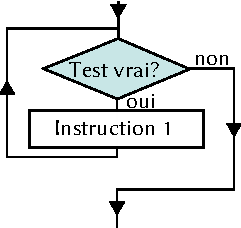
\includegraphics[scale=1.5]{images/Cf-while-fr.pdf}
\caption{Diagramme d'une boucle tant que}
\label{fig:Cf-while-fr}
\end{figure}

Cet algorithme\footnote{Un algorithme est un ensemble d'opérations ordonné qui permet de réaliser une opération plus complexe.} peut aussi être écrit\footnote{Ces exemples se veulent didactiques, nous verrons plus tard comment ces écritures peuvent être condensées.}:

\begin{Verbatim}[frame=single,rulecolor=\color{gray}, label=ne pas saisir]
>>> marche = 0
>>> while marche < 10001:
...     print(step)
...     if fatigué():
...         break
...     elif mauvais_temps():
...         break
...     else:
...         marche = marche + 1 
\end{Verbatim}

Tant que «~\texttt{marche}~» vaut moins de 10001 (tant que nous ne sommes pas arrivés) le bloc de code sera exécuté. Dans le bloc nous affichons la valeur de «~\texttt{marche}~» puis nous vérifions si nous sommes fatigués ou si le temps est mauvais. Si c'est le cas l'instruction «~\texttt{break}~» nous fait sortir de la boucle (nous sautons hors de la boucle à la ligne qui suit le bloc). Sinon nous ajoutons un à marche puis la condition de la boucle est contrôlée à nouveau.

Le mot \emph{break} signifie casser en anglais, \emph{break out}, s'évader.\\


Les étapes d'une boucle «~tant que~» sont simplement:
\begin{itemize}
\item vérifier la condition;
\item exécuter le code dans le bloc;
\item répéter.
\end{itemize}

Le plus souvent, une boucle tant que prendra en compte plusieurs conditions à la fois:

\begin{Verbatim}[frame=single,rulecolor=\color{gray}, label=ne pas saisir]
>>> marche = 0
>>> while marche < 10001 and en_forme() and beau_temps():
...     print(step)
...     marche = marche + 1 
\end{Verbatim}

Ou moins imagé mais que vous pouvez saisir tout de suite:

\begin{Verbatim}[frame=single,rulecolor=\color{mbleu}, label=à taper]
>>> x = 45
>>> y = 80
>>> while x < 50 and y < 100:
...     x = x + 1
...     y = y + 1
...     print(x, y)
\end{Verbatim}

Avant cette boucle nous créons une variable «~\texttt{x}~»  initialisé à 45 et une variable «~\texttt{y}~» initialisé à 80. Deux conditions doivent être vraies pour que le bloc de la boucle soit exécuté: x vaut moins de 50 et y moins de 100. Tant que les deux conditions sont vraies le bloc de code est exécuté. Ce bloc ajoute un aux deux variables et les affiche. Le résultat est juste:

\begin{Verbatim}[frame=single,rulecolor=\color{gray}, label=ne pas saisir]
46 81
47 82
48 83
49 84
50 85
\end{Verbatim}

Peut-être vous demandez-vous pourquoi ces nombres et seulement ces nombres sont imprimés?\\

Nous commençons à compter à partir de 45 pour «~\texttt{x}~»  et de 80 pour «~\texttt{y}~». Puis nous incrémentons (ajoutons un) à chaque variable à chaque «~tour~» de boucle. Le contrôle des conditions vérifie que x fait moins de 50 et y fait moins de 100. Après avoir parcouru la boucle cinq fois (en ajoutant un à chaque variable) la valeur de x atteint cinquante. Maintenant la première condition «~\texttt{x < 50}~»  est fausse donc Python arrête de boucler.

Un autre usage courant des boucle tant que est de créer des boucles semi-éternelles. 
Il s'agit de boucles qui s'exécutent pour toujours ou du moins jusqu'à ce quelque chose arrive dans le code qui va l'arrêter. Par exemple:

\begin{Verbatim}[frame=single,rulecolor=\color{gray}, label=ne pas saisir]
>>> while True:
...     plein de code ici
...     plein de code ici
...     plein de code ici
...     if une_condition == True:
...         break
\end{Verbatim}

La condition pour cette boucle tant que est juste «~\texttt{True}~» (vrai). Ainsi le code du bloc va toujours s'exécuter (c'est pourquoi la boucle est dite éternelle ou infinie). Néanmoins, si la variable «~\texttt{une\_condition}~»   devient vraie alors le code sortira de la boucle grâce à l'instruction «~\texttt{break}~». Vous trouverez un meilleur exemple de ce type de boucle infinie dans l'annexe C (dans la section à propos du module «~\texttt{random}~»  ) mais vous devriez attendre d'avoir lu le prochain chapitre avant d'y jeter un coup d'œil.

\section{À vous de jouer\label{PRATIQUE:BOUCLES}}
Dans ce chapitre nous avons vu comment utiliser des boucles pour réaliser des actions répétitives. Nous avons utilisé des blocs de code à l'intérieur de boucle pour les taches à répéter.


Vous trouverez des pistes de réponses dans la \autoref{REPONSES:BOUCLES}.
\subsection{Exercice 1}
Que pensez vous qu'il va arriver avec le code suivant?
\begin{Verbatim}[frame=single,rulecolor=\color{mbleu}, label=à taper]
>>> for x in range(0, 20):
... 	print('x vaut %s' % x)
... 	if x < 9:
... 		break
\end{Verbatim}

\subsection{Exercice 2}
Un lac est envahi par des nénuphars issus d'un jardin. Le premier jour un seul nénuphar est présent dans le lac.
Tous les jours le nombre de nénuphars double (est multiplié par deux). 
Sachant que le lac sera complètement envahi quand il y aura plus de mille nénuphars, combien de jours faut-il pour arriver à ce stade?

 \vfill
\begin{center}
 
\includegraphics[width=5cm]{images/sem2.pdf}
\end{center}
 \vfill

%\newpage
 
% \AddToShipoutPicture*{
% \put(0,0){
% \parbox[b][\paperheight]{\paperwidth}{

% }}}
\clearemptydoublepage

% This work is licensed under the Creative Commons Attribution-Share Alike 2.0 France License.
% To view a copy of this license, visit http://creativecommons.org/licenses/by-sa/2.0/fr/legalcode
% or send a letter to Creative Commons, 171 Second Street, Suite 300, San Francisco, California, 94105, USA.



\chapter{Une sorte de recyclage}
\section{De l'importance du recyclage}
Pensez à tous les déchets que vous créez chaque jour. Les bouteilles d'eau et d'autres boissons, les paquets de chips, les emballages en plastiques, les sacs en plastique pour les légumes, la viande en emballage plastique, les sacs de course, les journaux, les magazines et ainsi de suite.\\

Maintenant pensez à ce qui arriverez si tous ces déchets étaient mis en pile sur votre pas de porte.

\begin{center}
 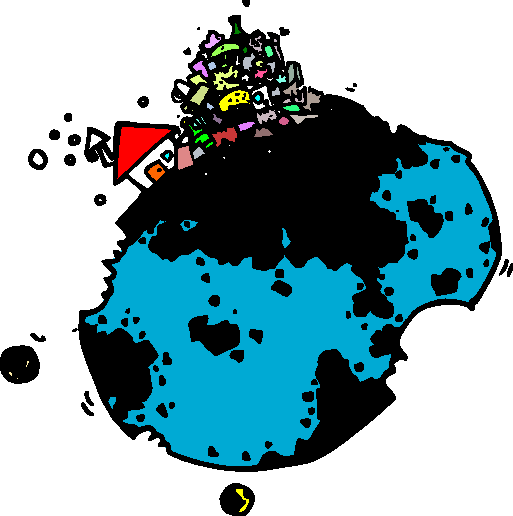
\includegraphics{images/recycler.pdf}
\end{center}

Bien sûr vous recyclez probablement autant que faire ce peut, ce qui est heureux, car personne n'aime devoir escalader un tas d'ordure pour aller à l'école. Ainsi les bouteilles en verres mises dans la poubelle pour le recyclage sont fondues et transformées en nouvelles bouteilles et saladiers. Le papier est transformé en papier recyclé. Le plastique est transformé en plastique dur et en polaires. C'est pourquoi votre pas de porte ne disparaît pas sous des tonnes de détritus.

Nous tendons à réutiliser des objets que nous créons plutôt que de creuser un gouffre sur la Terre pour fabriquer les mêmes choses encore et encore.

Recycler ou réutiliser dans le monde la programmation est aussi important. Non pas car votre programme va disparaître sous une pile d'immondices, mais si vous ne réutilisez pas une partie de ce que vous faites, vous ne pourrez plus utiliser vos doigts qui seront trop douloureux à cause de toute cette dactylographie.

Il y a de nombreuses manières différentes de réutiliser du code en Python (et dans les langages de programmation en général). Nous avons déjà aperçu certaines de ces manières avec le module «~\texttt{turtle}~»  et avec les fonctions «~\texttt{print}~» et «~\texttt{range}~».

Les fonctions sont une manière de réutiliser du code. Ainsi si vous pouvez écrire du code une fois puis l'utiliser dans vos programmes encore et encore. Commençons par essayer un exemple simple de fonction:

\begin{Verbatim}[frame=single,rulecolor=\color{mbleu}, label=à taper]
>>> def mafonction(un_nom):
...     print('Bonjour %s' % un_nom)
...
\end{Verbatim}

La fonction ci dessus a pour nom «~\texttt{mafonction}~» et pour paramètre «~\texttt{un\_nom}~».
Un paramètre est une variable qui est seulement disponible à l'intérieur du «~corps~» de la fonction. 
C'est à dire dans le bloc qui est directement après la ligne qui commence par «~\texttt{def}~». Au cas où vous vous poseriez la question «~\texttt{def}~»  est utiliser pour \emph{define} c'est à dire définir. Vous pouvez utiliser une fonction en l'appelant par son nom (défini juste après le «~\texttt{def}~») accolé à des parenthèses  qui entourent la valeur passée en paramètre:

\begin{Verbatim}[frame=single,rulecolor=\color{mbleu}, label=à taper]
>>> mafonction('Thaïs')
Bonjour Thaïs
>>> mafonction('Fripon')
Bonjour Fripon
\end{Verbatim}

Nous pouvons définir une fonction pour qu'elle prenne plusieurs paramètres, par exemple deux:

\begin{Verbatim}[frame=single,rulecolor=\color{mbleu}, label=à taper]
>>> def mafonction(prénom, nom):
...     print('Bonjour %s %s' % (prénom, nom))
...
\end{Verbatim}

Puis nous pour l'utiliser d'une manière similaire:

\begin{Verbatim}[frame=single,rulecolor=\color{mbleu}, label=à taper]
>>> mafonction('Élodie','Dupont')
Bonjour Élodie Dupont
\end{Verbatim}

Nous pouvons aussi créer des variables et appeler la fonction avec des variables:

\begin{Verbatim}[frame=single,rulecolor=\color{mbleu}, label=à taper]
>>> prénom_copain = 'Caroline'
>>> nom_copain = 'Robertson'
>>> mafonction(prénom_copain, nom_copain)
Bonjour Caroline Robertson
\end{Verbatim}

Nous pouvons, de plus, utiliser la déclaration «~\texttt{return}~» (retourner) pour retourner des valeurs:

\begin{Verbatim}[frame=single,rulecolor=\color{mbleu}, label=à taper]
>>> def économies(ménage, journeaux, dépenses):
...     return ménage + journeaux - dépenses
...
>>> print(économies(10, 10, 5))
15
\end{Verbatim}

Cette fonction prend trois paramètres puis additionne les deux premiers avant de soustraire le dernier (dépenses). Le résultat est alors retourné et peut utilisé comme paramètre d'une autre fonction (ici «~\texttt{print}~»).

Ce résultat peut aussi être utilisé pour initialiser une variable de la même manière que n'importe qu'elle valeur.

\begin{Verbatim}[frame=single,rulecolor=\color{mbleu}, label=à taper]
>>> mes_économies = économies(20, 10, 5)
>>> print(mes_économies)
25
\end{Verbatim}

Néanmoins, une variable que nous utilisons à l'intérieur du corps d'une fonction n'est pas accessible (utilisable) une fois que l'exécution est finie:

\begin{Verbatim}[frame=single,rulecolor=\color{red}, label=erreur]
>>> def test_variable():
...     a = 10
...     b = 20
...     return a * b
...
>>> print(variable_test())
200
>>> print(a)
Traceback (most recent call last):
File "<stdin>", line 1, in <module>
NameError: name 'a' is not defined
\end{Verbatim}

Dans l'exemple ci-dessus nous créons une fonction «~\texttt{test\_variable}~» qui multiplie deux variables «~\texttt{a}~» et «~\texttt{b}~» puis retourne le résultat. Si nous appelons cette fonction comme paramètre de «~\texttt{print}~»  nous avons pour réponse 200. Mais si nous appelons «~\texttt{print}~» pour afficher le contenu de «~\texttt{a}~» nous aurons  le message d'erreur «~\texttt{'a' is not defined}~» ('a' n'est pas défini). En programmation, l'endroit où est utilisable une variable est appelé la «~portée~» de cette variable.

Pensez à une petite île au milieu de l'océan trop éloignée de tout pour quitter l'île à la nage. Occasionnellement un avion vole au dessus et largue des feuilles de papier sur l'île (les paramètres de la fonction) que les habitants collent ensembles pour constituer un message qu'ils mettent dans une bouteille et jettent la bouteille à la mer (la valeur retournée). Ce que font les insulaire (ou les îliens en Bretagne) sur l'île et combien sont-ils pour faire le message, ne fait aucune différence pour la personne qui va ramasser la bouteille et lire le message qui était dedans. C'est sûrement la manière la plus simple de se représenter ce qu'est la portée. Mais il y a un petit problème avec cette représentation. Un des insulaire possède des jumelles très puissante (et l'île est proche de la côte) il peut ainsi voir le continent. Il peut même voir ce que font les continentaux et cela peut changer le message que les insulaires écrivent.

 \begin{Verbatim}[frame=single,rulecolor=\color{mbleu}, label=à taper]
>>> x = 100
>>> def test2_variable():
...     a = 10
...     b = 20
...     return a * b * x
...
>>> print(test2_variable())
20000
\end{Verbatim}

Ainsi même si les variables a et b ne peuvent pas être utilisée en dehors de la fonction la variable x qui a été créée hors de la fonction, est utilisable à l'intérieur. Essayez de penser à l'insulaire avec des jumelles et il est possible que cette image vous aidera un peu à bien comprendre les portées. 

\begin{center}
 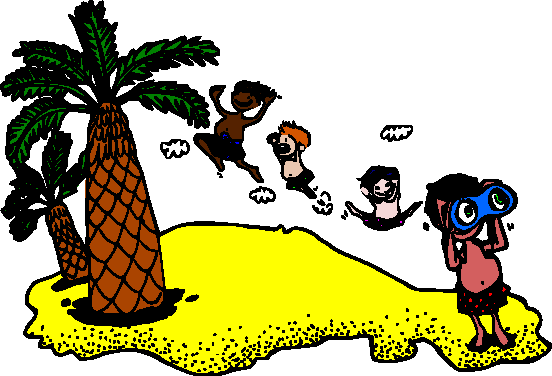
\includegraphics{images/ile.pdf}
\end{center}

L'itérateur que nous avions créé plus tôt pour afficher les économies durant une année peut facilement être intégré dans une fonction.

\begin{Verbatim}[frame=single,rulecolor=\color{mbleu}, label=à taper]
>>> def économies_annuelles(ménage, journaux, dépenses):
...     économies = 0
...     for semaine in range(1, 53):
...         économies += ménage + journaux - dépenses
...     print('Semaine %s = %s' % (semaine, économies))
...
\end{Verbatim}

Nous pouvons alors utiliser la fonction «~\texttt{économies\_annuelles()}~» :

\begin{Verbatim}[frame=single,rulecolor=\color{mbleu}, label=à taper]
>>> économies_annuelles(10, 10, 5)
Semaine 1 = 15
Semaine 2 = 30
Semaine 3 = 45
Semaine 4 = 60
Semaine 5 = 75
Semaine 6 = 90
Semaine 7 = 105
Semaine 8 = 120
Semaine 9 = 135
Semaine 10 = 150
[...]
\end{Verbatim}

Puis nous pouvons l'utiliser encore:

\begin{Verbatim}[frame=single,rulecolor=\color{mbleu}, label=à taper]
>>> économies_annuelles(25, 15, 10)
Semaine 1 = 30
Semaine 2 = 60
Semaine 3 = 90
Semaine 4 = 120
Semaine 5 = 150
[...]
\end{Verbatim}

Ce qui est plus pratique que de retaper l'itérateur à chaque fois que vous voulez essayer des valeurs différentes.
Les fonctions peuvent, par ailleurs, être groupées ensemble dans des choses appelés «~modules~»  qui sont \emph{très} utiles en Python et non pas moyennement utiles.\\

\emph{Plus à propos des modules, bientôt...}

\section{Modules}
Nous avons déjà vu quelques différentes manières de réutiliser du code. L'une d'elles est la fonction. Nous pouvons créer nous-mêmes des fonctions au sein de nos programmes ou utiliser les fonctions de base de Python comme «~\texttt{print}~», «~\texttt{range}~» «~\texttt{int}~» ou «~\texttt{str}~». 

Une autre méthode est d'utiliser des fonctions associées à des objets que nous appelons en utilisant le point «~\texttt{.}~»\footnote{Nous verrons ultérieurement les méthodes}.
 
Il est aussi possible d'utiliser des modules qui sont une manière de grouper des fonctions et des objets ensembles de manière utile.

Un exemple de module est le module «~\texttt{time}~», c'est à dire «~temps~»   en anglais:

\begin{Verbatim}[frame=single,rulecolor=\color{mbleu}, label=à taper]
>>> import time
\end{Verbatim}

La commande «~\texttt{import}~» est utilisée pour dire à Python que nous voulons accéder à un module.
Dans l'exemple ci-dessus, nous disons que nous voulons utiliser le module «~\texttt{time}~».
Nous pouvons alors appeler les fonctions et les objets qui sont disponibles dans ce module en utilisant le symbole du point «~\texttt{.}~», comme dans l'exemple ci-après:

\begin{Verbatim}[frame=single,rulecolor=\color{mbleu}, label=à taper]
>>> print(time.localtime())
time.struct_time(tm_year=2009, tm_mon=3, tm_mday=19, tm_hour=23, 
tm_min=22, tm_sec=4, tm_wday=3, tm_yday=78, tm_isdst=0)
\end{Verbatim}

La fonction «~\texttt{localtime}~» est une fonction interne au module «~\texttt{time}~» qui retourne l'heure et la date actuelle, découpées en année (\emph{year}), mois (\emph{month}), jour dans le mois «~\texttt{month day}~», heure (\emph{hour}), minutes (\emph{minutes}), secondes (\emph{seconds}), jour dans la semaine à compté de 0 pour lundi(\emph{week day}), jour dans l'année (\emph{year day}), et une indication d'un éventuel ajustement de l'heure).

Ces éléments sont stockés dans un n-uplet (voir la \autoref{sec:nuplets} page \pageref{sec:nuplets}). Nous pouvons utiliser une autre fonction du module pour avoir quelque chose de plus compréhensible:

\begin{Verbatim}[frame=single,rulecolor=\color{mbleu}, label=à taper]
>>> t = time.localtime()
>>> print(time.asctime(t))
Sat Nov 18 22:37:15 2006
\end{Verbatim}

Nous pouvons aussi utiliser les deux fonctions chaînées sur la même ligne:

\begin{Verbatim}[frame=single,rulecolor=\color{mbleu}, label=à taper]
>>> print(time.asctime(time.localtime()))
Sat Nov 18 22:37:15 2006
\end{Verbatim}

Tout cela est bien beau mais la date est en anglais! Cela est du au fait que la commande «~\texttt{time.asctime()}~» fournit la date en caractères ASCII (American Standard Code for Information Interchange). Comme vous pouvez le voir \autoref{tab:ascii} de nombreux caractères usuels en français et dans de nombreuses autres langues ne sont pas présents dans cette table. Néanmoins l'usage de l'ASCII perdure car il garantit la bonne compréhension par tous les types d'ordinateurs ou assimilés.

\begin{table}[h!]
\tt
\centering
\begin{tabular}{|c|c|c|c|c|c|c|c|c|c|}
\hline 
\verb*+ + & \verb+!+ & " & \# & \$ & \% & \& & ' & ( & ) \\ 
\hline
* & + & , & - & \verb+.+ & / & 0 & 1 & 2 & 3 \\ 
\hline
4 & 5 & 6 & 7 & 8 & 9 & \verb+:+ & \verb+;+ & $<$ & = \\ 
\hline
$>$ & \verb+?+ & @ & A & B & C & D & E & F & G \\ 
\hline
H & I & J & K & L & M & N & O & P & Q \\ 
\hline
R & S & T & U & V & W & X & Y & Z & [ \\ 
\hline
$\backslash$ & ] & \textasciicircum & \_ &  & ` & a & b & c & d \\ 
\hline
e & f & g & h & i & j & k & l & m & n \\ 
\hline
o & p & q & r & s & t & u & v & w & x \\ 
\hline
y & z & \{ & | & \} & \textasciitilde &  &  &  &  \\ 
\hline
\end{tabular}
\rm
\caption{caractères ASCII imprimables} \label{tab:ascii}
\end{table}

Heureusement Python sait aussi parler d'autres langues dont le français. Le module «~\texttt{locale}~» permet de localiser un certain nombre de fonctions:

\begin{Verbatim}[frame=single,rulecolor=\color{mbleu}, label=à taper]
>>> import locale
>>> locale.setlocale(locale.LC_ALL,'')
\end{Verbatim}

Nous indiquons ici à Python d'utiliser la langue utilisée par votre système d'exploitation (Windows dans votre cas) qui est probablement le français.

Puis nous pouvons utiliser la fonction «~\texttt{time.strftime()}~» qui permet un grand nombre de mises en forme\footnote{La fonction «~\texttt{time.strftime()}~» est décrite de manière plus détaillée en annexe.}:

\begin{small}
\begin{Verbatim}[frame=single,rulecolor=\color{mbleu}, label=à taper]
>>> temps=time.strftime('Nous somme le %A %d %B %Y et il est %H h %M min et %S s')
>>> print(temps)
Nous somme le jeudi 19 mars 2009 et il est 23 h 28 min et 24 s
\end{Verbatim}
\end{small}

Supposons que vous voulez demander à quelqu'un d'entrer ne valeur. Vous pouvez faire cela en utilisant la fonction
«~\texttt{print}~» et le module «~\texttt{sys}~» importé de la même manière que nous avions importé le module «~\texttt{time}~»: 

\begin{Verbatim}[frame=single,rulecolor=\color{mbleu}, label=à taper]
>>> import sys
\end{Verbatim}

À l'intérieur du module «~\texttt{sys}~» un objet appelé «~\texttt{stdin}~» pour \emph{standard input}.

Le mot \emph{standard input} est le terme anglais pour «~entrée standard~».

L'objet «~\texttt{stdin}~» a une méthode (ou fonction) vraiment utile appelé  «~\texttt{readline}~» qui est utiliser pour lire (\emph{read}) une ligne (\emph{line}) de texte que quelqu'un a tapé sur le clavier (après qu'il ait tapé sur la touche «~\texttt{Entrée}~». Vous pouvez tester «~\texttt{readline}~» en entrant la commande suivante dans la console Python:

\begin{Verbatim}[frame=single,rulecolor=\color{mbleu}, label=à taper]
>>> print(sys.stdin.readline())
\end{Verbatim}

Si vous tapez des mots et que vous pressez la touche entrée ce que vous venez de taper sera réaffiché. Repensons au code que nous avions écrit plus tôt en utilisant le test si:

\begin{Verbatim}[frame=single,rulecolor=\color{gray}, label=ne pas saisir]
>>> if âge >= 10 and âge <= 13:
...     print('Vous avez %s ans.' % âge)
... else:
...     print('Heu ?')
\end{Verbatim}

Plutôt que de créer une variable \texttt{âge} et de l'initialiser avec une valeur avant de l'utiliser nous pouvons  entrer une valeur au moment de la création de celle-ci au lancement d'une fonction:

\begin{Verbatim}[frame=single,rulecolor=\color{mbleu}, label=à taper]
>>> def votre_âge(âge):
...     if âge >= 6 and âge <= 13:
...         print('Vous avez %s ans.' % âge)
...     else:
...         print('Heu ?')
...
\end{Verbatim}

Notre fonction «~\texttt{votre\_âge()}~» peut être appelée en passant un nombre comme valeur en paramètre. Nous allons tester que cela fonctionne correctement: 

\begin{Verbatim}[frame=single,rulecolor=\color{mbleu}, label=à taper]
>>> votre_âge((9)
Heuh ?
>>> votre_âge((10)
Vous avez 10 ans.
\end{Verbatim}

Maintenant que nous savons qu'il n'y a pas de problème avec notre fonction, nous pouvons,
avec «~\texttt{readline}~», demander à quelqu'un d'entrer son âge.


\begin{Verbatim}[frame=single,rulecolor=\color{mbleu}, label=à taper]
>>> def votre_âge():
...     print('S'il vous plait entrez votre âge :')
...     âge = int(sys.stdin.readline())
...     if age >= 6 and age <= 13:
...         print('Vous avez %s ans.' % âge)
...     else:
...         print('Heu ?')
...
\end{Verbatim}

Comme «~\texttt{readline}~» retourne ce que la personne a entré comme texte, c'est à dire une chaîne, nous avons besoin de convertir cette chaîne en nombre avec la fonction «~\texttt{int}~». Une fois converti en nombre nous pouvons utiliser la valeur stockée en utilisant «~\texttt{âge}~» dans un test si (vous pourrez trouver des informations à ce sujet \autoref{sec:dif}, page \pageref{sec:dif}).

Maintenant essayons notre fonction, appelez  «~\texttt{votre\_âge()}~» sans paramètre et le texte que vous aviez indiqué va apparaître:

\begin{Verbatim}[frame=single,rulecolor=\color{mbleu}, label=à taper]
>>> votre_âge()
S'il vous plait entrez votre âge :
6
Vous avez 6 ans.
>>> votre_âge()
S'il vous plait entrez votre âge :
15
Heu ?
\end{Verbatim}

Deux choses sont importantes à noter:
\begin{itemize}
\item «~\texttt{readline}~» renvoie toujours une chaîne de caractères;
\item notre fonction ne fonctionne que si vous entrez des entiers (nous verrons plus tard comme régler ce problème).
\end{itemize}

Les modules «~\texttt{sys}~»  et «~\texttt{time}~»  sont juste l'un des nombreux modules inclus dans Python. Vous trouverez plus d'information sur certains modules Python (mais pas tous) en \autoref{annexe:mod}.

\section{À vous de jouer\label{pratique:recyclage}}
Dans ce chapitre nous avons vu comment recycler des choses en Python en utilisant des fonctions et des modules.
Nous verrons dans le chapitre suivant comment sauver vos programmes pour pouvoir les réutiliser ou les faire utiliser par d'autres personnes.

Nous avons évoqué la «~portée~» d'une variable, c'est à dire que les variables extérieures aux fonctions peuvent être utilisées à l'intérieur de celles-ci, alors que les variables définies à l'intérieur des fonctions ne pouvaient pas être utilisées à l'extérieur de celles-ci.

Nous avons aussi appris à créer des fonctions avec «~\texttt{def}~».

Vous trouverez des pistes de réponses dans la \autoref{reponses:recyclage}.


\subsection{Exercice 1}
Dans le deuxième exercice du \autoref{pratique:boucles}, nous avions créé un itérateur pour calculer la prolifération des nénuphars jusqu'à ce qu'il y ait milles nénuphars dans l'étang.
Essayez de créer une fonction qui prend comme paramètres:
\begin{itemize}
\item le nombre initial de nénuphar;
\item le coefficient de reproduction quotidien (par combien le nombre de nénuphars est multiplié tout les jours).
\end{itemize}
Vous pouvez appeler cette fonction de la manière suivante «~\texttt{calcul\_nénuphars(2,1.5)}~».

\subsection{Exercice 2}
Prenez la fonction que vous venez de créer et modifiez la de manière à pouvoir calculer le nombre de nénuphars pour différents nombres de jours pour lesquels nous voulons un résultat.
Vous pouvez appeler cette fonction de la manière suivante «~\texttt{calcul\_nénuphars(2,1.5)}~» 

\subsection{Exercice 3}
Plutôt qu'une simple fonction dans laquelle nous passons les valeurs en paramètre, nous pouvons faire un mini-programme qui demande à quelqu'un les valeurs en utilisant la fonction «~\texttt{sys.stdin.readline()}~».

Dans ce cas nous appellerons la fonction sans paramètre du tout «~\texttt{calcul\_nénuphars()}~».

De manière à créer cette fonction et si nous voulons pourvoir entrer des nombres à virgule, il convient de remplacer la fonction «~\texttt{int}~» par la fonction «~\texttt{float}~» dont nous n'avons pas encore parlé.
Cette fonction convertit une chaîne en nombre dit à virgule flottante (nombre rationnel dont nous avons parlé brièvement au \autoref{chap:8} page \pageref{chap:8}). Les nombre à virgule sont représentés en Python en utilisant un point «~\texttt{.}~» comme «~\texttt{20.3}~» pour 20,3 ou «~\texttt{2541.933}~»  pour 2541,933.


 \vfill
\begin{center}
 
\includegraphics[width=5cm]{images/ourochin.pdf}
\end{center}
 \vfill

% This work is licensed under the Creative Commons Attribution-Share Alike 2.0 France License.
% To view a copy of this license, visit http://creativecommons.org/licenses/by-sa/2.0/fr/legalcode
% or send a letter to Creative Commons, 171 Second Street, Suite 300, San Francisco, California, 94105, USA.



\chapter{Un court chapitre à propos des fichiers}
\section{Sauvegarde des programmes}

Vous savez déjà probablement ce qu'est un fichier ( \emph{file} en anglais pour l'informatique).
Dans votre classe vous avez probablement des fiches ---par exemple de lecture, de botanique--- qui sont réunies ensembles au sein de fichiers. Ces fichiers sont réunis dans des boites pour faciliter leur utilisation.

En informatique les choses sont assez similaires, nous mettons les informations dans des fichiers que nous rangeons dans des répertoires (appelés aussi dossiers), la \autoref{fig:Files11_directory_hierarchy} montre cette organisation.

\begin{figure}[h!]
\centering
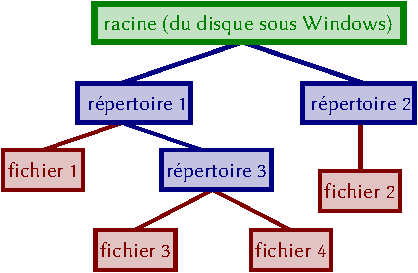
\includegraphics[scale=1]{images/Files11_directory_hierarchy.pdf}
\caption{Organisation des fichiers et des répertoires}\label{fig:Files11_directory_hierarchy}
\end{figure}


Rappelez-vous au premier chapitre nous avions créé un fichier «~\texttt{bonjour.py}~» et nous ne pouvions pas voir le résultat de l'exécution de programme.

Nous allons maintenant voir comment utiliser ce type de fichier.
Premièrement cliquez droit sur le fichier bonjour.py et choisissez «~\texttt{éditer avec IDLE}~» comme sur la \autoref{fig:edit_idle}.
\begin{figure}[h!]
\centering
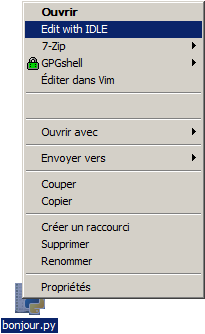
\includegraphics[scale=0.5]{images/edit_idle.png} 
\caption{Édition avec IDLE}
\label{fig:edit_idle}
\end{figure}

Deux fenêtres s'ouvrent alors: l'éditeur et le shell comme montrés sur 
la \autoref{fig:ouvert_idle}.
\begin{figure}[h!]
\centering
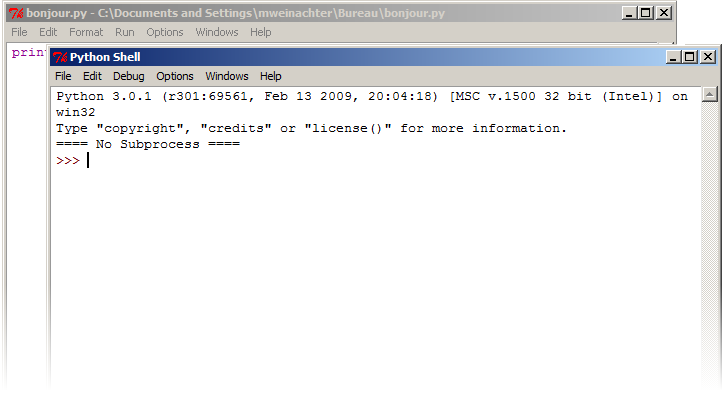
\includegraphics[scale=0.5]{images/ouvert_idle.png} 
\caption{Fenêtres d'IDLE}
\label{fig:ouvert_idle}
\end{figure}

Selon vos préférences vous pouvez afficher l'une ou l'autre des fenêtres . \\

\emph{En tant que livre je préfère une présentation de type une page à gauche et
 une page à droite. Pour ce faire je clique droit sur la barre des tâches et je choisis mosaïque verticale.}\\

Comme vous le voyez le code que vous aviez entré est affiché dans la fenêtre «~Bonjour.py~». Sélectionnez cette fenêtre puis appuyez sur la touche «~\texttt{F5}~» ou cliquez sur «~\texttt{Run}~» (courir en anglais normal, exécuter en informatique) puis «~\texttt{run module}~». Le résultat s'affiche dans le shell.

Comme vous le voyez vous pouvez éditer, sauvegarder et réutiliser le code que vous réalisez.

Modifier le code comme suit: 

\begin{Verbatim}[frame=single,rulecolor=\color{mbleu}, label=à taper]
import sys

print("Bonjour le monde")
sys.stdin.readline()
\end{Verbatim}

Puis lancez le avec la touche «~\texttt{F5}~» l'éditeur va vous demander de sauvegarder le fichier pour pouvoir l'exécuter, répondez oui car c'est ce que nous voulons. Le programme s'exécute et attend que vous appuyez sur entrée. Plus intéressant vous pouvez double-cliquer sur le fichier «~\texttt{bonjour.py}~». Le message s'affiche et reste affiché. \\

\emph{Vous pouvez si vous le souhaiter compléter ce programme et le montrer facilement à la personne qui m'a offert à vous. Par exemple vous pouvez poser une question et composer une réponse à partir de celle-ci.}\\

\section{Si on ça ne passe pas la fenêtre, passons par le soupirail}
Microsoft a décidé au cours des évolutions de son système d'exploitation de changer les endroits (répertoires) utilisés pour le bureau et les documents. Ces répertoires dont le nom était traduit, ont maintenant toujours des noms anglais.

De plus certains chemins simples d'accès comme «~\Verb+C:\+~» ne sont plus toujours accessibles pour des raisons de sécurité.

Il existe des modules qui permettent à Python de connaitre le chemin vers votre bureau ou votre répertoire personnel sans programmation mais ils nécessiteraient une installation supplémentaire. Or nous ne voulons pas déranger vos parents (ou assimilés) à nouveau... Ils sont tellement bien tranquilles sur le canapé.

Nous pourrions aussi sans programmation créer un raccourci sur le bureau pour que vous puissiez accéder facilement à votre répertoire personnel qui contient le «~\texttt{bureau}~»  et «~\texttt{mes documents}~». Cette solution est présentée pour information \autoref{fig:etapesra} page \pageref{fig:etapesra}. Mais cette solution est assez longue et finalement assez éloignée de mon sujet.

\begin{figure}[h!tb]
\centering
%\subfigure[Caption of subfigure 1]{
%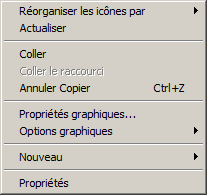
\includegraphics[scale=0.5]{images/clickdb.png}
%\label{fig:subfig1}
%}
\subfigure[Clic droit sur le bureau]{
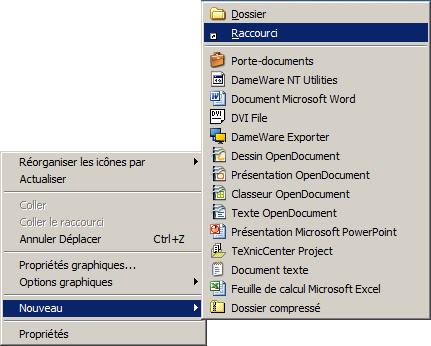
\includegraphics[scale=0.5]{images/nouvra.png}
\label{fig:nouvra}
}
\subfigure[Entrée de «~\texttt{\%userprofile\%}~»]{
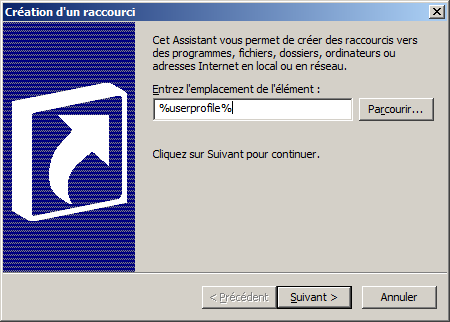
\includegraphics[scale=0.5]{images/creara.png}
\label{fig:creara}
}
\subfigure[Nom du raccourci par défaut]{
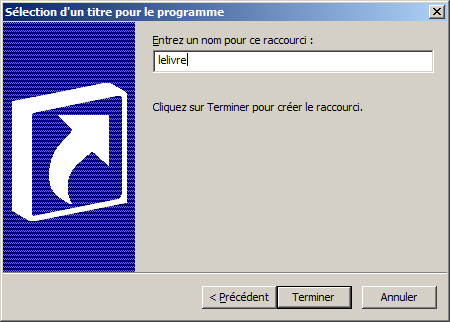
\includegraphics[scale=0.5]{images/comptera.png}
\label{fig:comptera}
}
\subfigure[Entrée de «~\texttt{maison}~»]{
\includegraphics[scale=0.5]{images/maison1.png}
\label{fig:maison1}
}

\subfigure[Le raccourci sur le bureau]{
\includegraphics[trim = -40mm 0mm -40mm 0mm, clip,scale=1]{images/maison2.png}
\label{fig:maison2}
}
\caption{Étapes de la création d'un raccourci vers le répertoire personnel}
\label{fig:etapesra}
\end{figure}


C'est pourquoi je vous propose de retrouver le chemin de votre bureau avec Python.
Dans le shell ou dans l'éditeur faites «~\texttt{Ctrl+N}~» ou «~\texttt{file}~» puis   
«~\texttt{New Window}~», une nouvelle fenêtre de l'éditeur s'ouvre alors.

Vous pouvez alors commencer par identifier la variante du système d'exploitation que vous utilisez:
\begin{Verbatim}[frame=single,rulecolor=\color{mbleu}, label=à taper]
import os,platform

print(platform.release())
print(os.environ['USERPROFILE'])
\end{Verbatim}

Après avoir tapé F5 et sauvegardé le fichier (avec l'extension «~\texttt{.py}~»)  vous devriez avoir quelque chose comme:

\begin{Verbatim}[frame=single,rulecolor=\color{gray}, label=résultat]
XP
C:\Documents and Settings\lelivre
\end{Verbatim}

Nous venons d'obtenir la version de Windows et le chemin vers votre répertoire personnel.
Utilisons alors ces données pour avoir le chemin vers votre bureau:

\begin{Verbatim}[frame=single,rulecolor=\color{mbleu}, label=à taper]
import os,platform

def chemin_bureau() :
    if platform.release()=='XP' :
        return os.path.join(os.environ['USERPROFILE'],"Bureau")
    else :
        return os.path.join(os.environ['USERPROFILE'],"Desktop")
\end{Verbatim}

Exécutons ce module: il ne se passe rien! C'est justement car le fichier que nous venons de créer est un module qui introduit une fonction «~\texttt{chemin\_bureau()}~» mais ne la lance pas. Nous devons modifier légèrement le fichier pour lancer la fonction et, par exemple, afficher le résultat:

\begin{Verbatim}[frame=single,rulecolor=\color{mbleu}, label=à taper]
import os,platform

def chemin_bureau() :
    if platform.release()=='XP' :
        return os.path.join(os.environ['USERPROFILE'],"Bureau")
    else :
        return os.path.join(os.environ['USERPROFILE'],"Desktop")
    
print(chemin_bureau())
\end{Verbatim}

Le résultat que vous devez obtenir doit ressembler à ce qui suit:

\begin{Verbatim}[frame=single,rulecolor=\color{gray}, label=résultat]
C:\Documents and Settings\lelivre\Bureau
\end{Verbatim}

Examinons ce que Python vient de faire. En premier Python importe deux modules «~\texttt{os}~» et «~\texttt{platform}~». Le module «~\texttt{platform}~» apporte des informations sur la plateforme qui sert à lancer les programmes (version du système d'exploitation par exemple). Le module «~\texttt{os}~» apporte une interface pour communiquer avec le système d'exploitation, \emph{operating system} en anglais.

Puis une fonction «~\texttt{chemin\_bureau}~» est créée qui ne prend aucun paramètre en entrée. Python regarde alors le type de Windows utilisé puis selon le résultat retourne le chemin vers le bureau au format approprié en joignant le chemin vers votre répertoire personnel et la chaîne utilisé par votre version de Windows pour identifier le bureau.

Enfin nous avons indiqué à Python que nous voulions qu'il affiche avec «~\texttt{print}~» le résultat de la commande «~\texttt{chemin\_bureau}~».

Dans un programme plus important on crée généralement une fonction «~\texttt{main}~» qui sera exécutée en premier. Cette convention facilite la lecture d'un programme par d'autres personnes.

\section{Un peu de lecture, maintenant?}
Quand Python est installé sur votre ordinateur, un tas de fonctions et de modules sont aussi installés. Certaines fonctions sont disponibles par défaut. La fonction «~\texttt{range}~» que nous avons déjà vu est de ce type. nous allons maintenant regarder la fonction «~\texttt{file}~» que nous n'avons pas encore utilisé.

Pour voir comment les fichiers sont utilisés ouvrez le bloc-notes  tapez quelques lignes et sauvez le fichier sur votre bureau:
\begin{enumerate}
\item cliquez sur le menu fichier puis enregistrer (ou simplement faites «~\texttt{Ctrl+S}~»);
\item cliquez sur Bureau;
\item dans le champ «~\texttt{nom du fichier}~» où il y a écrit «~\texttt{*.txt}~», tapez «~\texttt{test.txt}~».
\end{enumerate}

Ouvrez le fichier qui contient la fonction «~\texttt{chemin\_bureau}~» (avec un clic droit «~\texttt{edit with IDLE}~» et essayez ce qui suit à la fin du fichier:
\begin{Verbatim}[frame=single,rulecolor=\color{mbleu}, label=à taper]
import os,platform

def chemin_bureau() :
    if platform.release()=='XP' :
        return os.path.join(os.environ['USERPROFILE'],"Bureau")
    else :
        return os.path.join(os.environ['USERPROFILE'],"Desktop")
    
fichier = open(os.path.join(chemin_bureau(),'test.txt'))
print(fichier.read())
\end{Verbatim}

Lancez le programme (avec «~\texttt{F5}~») et le contenu du fichier que vous venez de créer devrait s'afficher dans le shell. 

Que peut bien faire ce code? La première ligne importe les modules «~\texttt{os}~»  et «~\texttt{platform}~». Les lignes 3 à 7 définissent la fonction pour le chemin vers le bureau.
La ligne 9 ouvre le fichier que vous venez tout juste de créer en utilisant le chemin vers le bureau et le nom du fichier.

La fonction «~\texttt{open}~»  crée un type de valeur particulier (appelé génériquement objet) qui représente le fichier. Dans le cas présent l'objet créé est de type «~\texttt{file}~» (c'est à dire fichier). La variable «~\texttt{fichier}~» pointe vers l'objet de type «~\texttt{file}~» que nous venons de créer.

La variable «~\texttt{fichier}~» n'est pas le fichier en lui-même mais une sorte de gros doigt qui pointe vers le fichier.

La dernière ligne appelle la fonction «~\texttt{read}~» propre aux objets de type «~\texttt{file}~». La fontion «~\texttt{read}~» lit le contenu du fichier et «~\texttt{print}~» l'affiche dans le shell. Parce que la variable «~\texttt{fichier}~» pointe vers un objet qui contient des informations et des fonctions (appelées méthodes pour des objets), nous devons utiliser le point «~\texttt{.}~»  pour utiliser ces méthodes disponibles dans l'objet.

\begin{center}
\fcolorbox{black}{lbleu}{
\begin{minipage}{12cm}
L'annexe \autoref{annexe:ref} (vers la fin de ce livre) contient plus d'information sur les commandes intégrées à Python.
\end{minipage}
 }
\end{center}

\section{Écrivons\\
En Python! (rime faible)}

Nous avons déjà créé un objet «~\texttt{file}~» dans la section précédente, en utilisant Python:

\begin{Verbatim}[frame=single,rulecolor=\color{gray}, label=ne pas saisir]
import os,platform

def chemin_bureau() :
    if platform.release()=='XP' :
        return os.path.join(os.environ['USERPROFILE'],"Bureau")
    else :
        return os.path.join(os.environ['USERPROFILE'],"Desktop")
    
fichier = open(os.path.join(chemin_bureau(),'test.txt'))
print(fichier.read())
\end{Verbatim}

Un objet «~\texttt{file}~» n'a pas seulement une fonction «~\texttt{read}~». Après tout un fichier ne serait pas très utile si on pouvait seulement prendre des fiches mais ne jamais en rajouter. Nous pouvons créer un nouveau fichier vide en passant un autre paramètre à la fonction «~\texttt{open}~».

Contrôlez d'abord qu'il n'existe pas de fichier «~\texttt{nouveau.txt}~» sur votre bureau. Si cela est le cas vous pouvez soit le renommer (par exemple en «~\texttt{ancien.txt}~» , soit changer «~\texttt{nouveau.txt}~» en ce que vous voulez dans les exemples qui suivent. Enfin, une fois ce contrôle effectué 

\begin{Verbatim}[frame=single,rulecolor=\color{mbleu}, label=à taper par exemple en reprenant l'existant]
import os,platform

def chemin_bureau() :
    if platform.release()=='XP' :
        return os.path.join(os.environ['USERPROFILE'],"Bureau")
    else :
        return os.path.join(os.environ['USERPROFILE'],"Desktop")
    
fichier = open(os.path.join(chemin_bureau(),'nouveau.txt'),'w')
\end{Verbatim}

Exécutez ce programmes puis regardez sur votre bureau, un fichier «~\texttt{nouveau.txt}~» vient d'être créé. Le paramètre «~\texttt{w}~» (pour \emph{write}, écrire en anglais) est utilisé pour indiquer à Python que nous voulons écrire dans un (nouveau) fichier. Si le fichier n'existe pas il est créé, s'il existe son contenu est détruit.

Nous pouvons maintenant utiliser la fonction «~\texttt{write}~». Une fois que nous aurons écrit il convient d'indiquer à Python que nous ne désirons plus écrire dans le fichier en utilisant la fonction «~\texttt{close}~» (\emph{close} signifie fermer en anglais). Notez au passage qu'il est de bon ton d'utiliser aussi la fonction «~\texttt{close}~» quand on finit d'utiliser un fichier.
 
\begin{Verbatim}[frame=single,rulecolor=\color{mbleu}, label=à taper par exemple en reprenant l'existant]
import os,platform

def chemin_bureau() :
    if platform.release()=='XP' :
        return os.path.join(os.environ['USERPROFILE'],"Bureau")
    else :
        return os.path.join(os.environ['USERPROFILE'],"Desktop")
    
fichier = open(os.path.join(chemin_bureau(),'nouveau.txt'),'w')
fichier.write('''Ceci est un fichier de test.
Ce fichier s'étend sur plusieurs lignes.
Trois en fait !''')
fichier.close()
\end{Verbatim}

Si vous ouvrez le fichier avec votre éditeur de texte favori (le bloc note à priori) vous verrez qu'il contient le texte:

\begin{Verbatim}[frame=single,rulecolor=\color{gray}, label=contenu de nouveau.txt]
Ceci est un fichier de test.
Ce fichier s'étend sur plusieurs lignes.
Trois en fait !
\end{Verbatim}

Ou mieux encore nous pouvons utiliser Python pour lire ce texte:

\begin{Verbatim}[frame=single,rulecolor=\color{mbleu}, label=à taper par exemple en reprenant l'existant]
import os,platform

def chemin_bureau() :
    if platform.release()=='XP' :
        return os.path.join(os.environ['USERPROFILE'],"Bureau")
    else :
        return os.path.join(os.environ['USERPROFILE'],"Desktop")
    
fichier = open(os.path.join(chemin_bureau(),'nouveau.txt'),'w')
fichier.write('''Ceci est un fichier de test.
Ce fichier s'étend sur plusieurs lignes.
Trois en fait !''')
fichier.close()

fichier = open(os.path.join(chemin_bureau(),'nouveau.txt'))
print(fichier.read())
fichier.close
\end{Verbatim}

À ce point quelque chose pourrait vous surprendre: le résultat de la commande ci-dessus reste nos trois lignes. Or nous avons écrit \emph{deux} fois dans le fichier. Que c'est-il passé?

L'ouverture en mode «~\texttt{w}~» indique que nous souhaitons écrire en écriture à partir de zéro. Le contenu initial du fichier a été détruit. Nous pouvons modifier le «~\texttt{w}~» en «~\texttt{a}~» pour \emph{append} qui signifie ajouter en anglais.

\begin{Verbatim}[frame=single,rulecolor=\color{mbleu}, label=à taper par exemple en reprenant l'existant]
import os,platform

def chemin_bureau() :
    if platform.release()=='XP' :
        return os.path.join(os.environ['USERPROFILE'],"Bureau")
    else :
        return os.path.join(os.environ['USERPROFILE'],"Desktop")
    
fichier = open(os.path.join(chemin_bureau(),'nouveau.txt'),'a')
fichier.write('''Ceci est un fichier de test.
Ce fichier s'étend sur plusieurs lignes.
Trois en fait !''')
fichier.close()

fichier = open(os.path.join(chemin_bureau(),'nouveau.txt'))
print(fichier.read())
fichier.close
\end{Verbatim}

Si nous exécutons ce programme le résultat devrait être:

\begin{Verbatim}[frame=single,rulecolor=\color{gray}, label=résultat en mode ajout]
Ceci est un fichier de test.
Ce fichier s'étend sur plusieurs lignes.
Trois en fait !Ceci est un fichier de test.
Ce fichier s'étend sur plusieurs lignes.
Trois en fait !
\end{Verbatim}

Bizarrement le résultat est sur cinq lignes et non pas six (deux fois trois). En fait quand nous saisissons le texte sur plusieurs lignes le caractère entrée que nous ne voyons pas est pris en compte. La dernière ligne ne finissait pas le caractère entrée et la première ne commençait pas par celui-ci.
Nous pouvons modifier la chaîne pour que les nouvelles lignes commencent par un retour à la ligne:

\begin{Verbatim}[frame=single,rulecolor=\color{mbleu}, label=à taper]
fichier.write('''
Ceci est un fichier de test.
Ce fichier s'étend sur plusieurs lignes.
Trois en fait !''')
\end{Verbatim}

Notez bien que pour alléger la notation l'ensemble du code de votre fichier n'a pas été repris. Par ailleurs et pour information, le retour à la ligne peut aussi être saisi «~\Verb+\n+~». Cette notation est simple à retenir : «~\Verb+\n+~» comme \textbf{n}ouvelle ligne.
\newpage
\thispagestyle{empty}
\AddToShipoutPicture*{
 \put(0,0){
 \parbox[b][\paperheight]{\paperwidth}{
 \vfill
\begin{center}
 \includegraphics[width=5cm]{images/Ouroboros-Zanaq.pdf}
\end{center}
 \vfill
 }}}


% This work is licensed under the Creative Commons Attribution-Share Alike 2.0 France License.
% To view a copy of this license, visit http://creativecommons.org/licenses/by-sa/2.0/fr/legalcode
% or send a letter to Creative Commons, 171 Second Street, Suite 300, San Francisco, California, 94105, USA.




\chapter{Tortues à profusion\label{chap:tortue2}}
\section{Le retour de la tortue}
Revenons au module tortue que nous avions commencé à examiner au \autoref{chap:tortue1} page \pageref{chap:tortue1}. Nous allons examiner tout un ensemble de fonctions du module turtle. 

Vous vous demandez peut-être comment avoir des informations sur toutes ces commandes, en fait Python inclut une aide interne (sans parler de l'aide disponible dans le menu démarrer). Vous pouvez faire «~\texttt{dir(turtle)}~» pour avoir la liste de toutes les commandes inclues dans turtle. La commande «~\texttt{dir}~» est disponible pour tous les modules. De plus les modules bien développés incluent une aide en ligne par exemple «~\texttt{help(turtle.Pen())}~». Cette aide est malheureusement pour les francophones en anglais. Néanmoins, cela pourrait être pire dans une langue dont vous  ne comprendriez même pas les caractères. Vous pouvez essayer ces commandes dans la console ou le shell:

\begin{Verbatim}[frame=single,rulecolor=\color{mbleu}, label=à taper]
>>> dir(str)
>>> help(str.isapha)
>>> import turtle
>>> dir(turtle)
>>> help(turtle.Pen)
\end{Verbatim}

Pour information, la méthode «~\texttt{isalpha}~» teste une chaine pour savoir si elle est composée de lettres uniquement et renvoie vrai «~\texttt{True}~» ou faux «~\texttt{False}~».

Revenons, à  nouveau, sur le module «~\texttt{turtle}~». Rappelez-vous, pour afficher une zone de dessin et dessiner dessus. Nous avions besoin d'importer le module «~\texttt{turtle}~» et de créer un objet «~\texttt{Pen}~»:
\begin{Verbatim}[frame=single,rulecolor=\color{gray}, label=ne pas saisir]
>>> import turtle
>>> tortue = turtle.Pen()
\end{Verbatim}

À l'époque nous fermions la fenêtre en lançant «~\texttt{turtle.bye()}~».

Maintenant que nous savons utiliser IDLE pour créer, exécuter et sauvegarder des programmes nous ne souhaitons pas ouvrir une  fenêtre de dessins a chaque exécution, la commande «~\texttt{turtle.bye()}~» permettrait de fermer la fenêtre dessin mais nous ne verrions plus le résultat de nos programmes c'est pourquoi je vous propose d'utiliser 
la méthode «~\texttt{turtle.exitonclick}~»  (\emph{exit} signifie sortie, \emph{on} signifie sur, \emph{click} signifie clic).

N'oubliez pas de créer une nouvelle fenêtre (\emph{new windows} dans le menu «~\texttt{File}~» d'IDLE ou de rouvrir un programme existant pour taper votre code.

\begin{Verbatim}[frame=single,rulecolor=\color{mbleu}, label=à taper]
import turtle
tortue = turtle.Pen()
tortue.forward(100)
turtle.exitonclick
\end{Verbatim}

Lancez le programme (sauvez le sous le nom de votre choix finissant par «~\texttt{.py}~» si nécessaire) puis cliquez sur la fenêtre de dessin pour quitter le programme.

Nous pouvons maintenant utiliser des fonctions simples pour déplacer notre tortue sur le zone de dessin et dessiner des formes simples. Mais encore plus intéressant nous pouvons utiliser ce que nous avons appris dans les chapitres précédents. Par exemple, le code que nous avions utilisé pour créer un carré était:

\begin{Verbatim}[frame=single,rulecolor=\color{gray}, label=ne pas saisir]
>>> tortue.forward(50)
>>> tortue.left(90)
>>> tortue.forward(50)
>>> tortue.left(90)
>>> tortue.forward(50)
>>> tortue.left(90)
\end{Verbatim}

Nous pouvons maintenant le ressaisir en utilisant un itérateur:

\begin{Verbatim}[frame=single,rulecolor=\color{mbleu}, label=à taper]
import turtle
tortue = turtle.Pen()
for x in range(4):
    tortue.forward(50)
    tortue.left(90)
    
turtle.exitonclick
\end{Verbatim}

Ce qui fait nettement moins à saisir, mais nous pouvons maintenant faire des choses un peu plus intéressantes. Essayez donc ce qui suit:
\begin{Verbatim}[frame=single,rulecolor=\color{mbleu}, label=à taper]
import turtle
tortue = turtle.Pen()
for x in range(8):
    tortue.forward(100)
    tortue.left(225)
    
turtle.exitonclick()
\end{Verbatim}

Ce code produit une étoile à huit branches comme montré sur la \autoref{fig:etoile8} (la tortue tourne de 225 degrés puis avance de 100 pixels, huit fois).
\begin{figure}[h!]
\centering
\includegraphics[scale=0.4]{images/etoile8}
\caption{Étoile à huit branches}\label{fig:etoile8}
\end{figure}


\section{Je jure [...] de dire \emph{toute} la vérité, rien que la vérité}

Comme nous avons pu le remarquer la tortue et lente, très lente... En fait on peut choisir la vitesse de la «~tortue~» avec la fonction «~\texttt{turtle.speed}~» (\emph{speed} signifie vitesse en anglais). La fonction «~\texttt{turtle.speed}~» prend en paramètre un entier entre zéro et dix. D'après le manuel, la vitesse de dessin va de très lent pour un, à très rapide pour dix. La vitesse normale (par défaut) est six. Pour une valeur de zéro aucune animation n'a lieu, c'est à dire que l'affichage du résultat est presque instantané:

\begin{Verbatim}[frame=single,rulecolor=\color{mbleu}, label=à taper]
import turtle
turtle.speed(0)
tortue = turtle.Pen()

for x in range(36):
    tortue.forward(200)
    tortue.left(170)
    
turtle.exitonclick()
\end{Verbatim}

Comme vous pouver le voir sur la \autoref{fig:etoile36} on obtient une étoile avec plein de branches.
\begin{figure}[h!]
\centering
\includegraphics[scale=0.4]{images/etoile36}
\caption{Étoile à trente six branches}\label{fig:etoile36}
\end{figure}

À ce point deux choses on pu vous surprendre:
\begin{itemize}
\item la vitesse la plus rapide est assez lente;
\item une flèche est apparue au début du dessin lors du lancement de l'instruction\\
«~\texttt{turtle.speed}~». 
\end{itemize}

En fait deux impressions expliquent ces constatations. Le système d'affichage interne de «~\texttt{turtle}~» est lent le terme instantané et donc très faux. deuxièmement l'instruction «~\texttt{turtle.Pen()}~» ne crée que par effet de bord une zone d'affichage. L'instruction «~\texttt{turtle.Pen}~» crée un stylo qui va écrire sur la zone de dessin. Si celle-ci n'existe pas elle est alors créée au passage. Inversement le module «~\texttt{turtle}~» inclut un stylo par défaut et «~\texttt{turtle.forward}~» créera un stylo pour réaliser une écriture.

Malheureusement l'instruction «~\texttt{turtle}~» créer aussi un stylo... Heureusement il existe des instructions pour cacher ou faire apparaître les stylos.

\begin{Verbatim}[frame=single,rulecolor=\color{mbleu}, label=à taper]
import turtle
turtle.hideturtle()
turtle.speed(0)

tortue = turtle.Pen()
tortue.hideturtle()


for x in range(36):
    tortue.forward(200)
    turtle.speed(0)
    tortue.left(170)

tortue.showturtle()    
turtle.exitonclick()
\end{Verbatim}

L'instruction «~\texttt{turtle.hideturtle()}~» cache le stylo par défaut (\emph{hide} cacher en anglais) plus généralement si une «~\texttt{variable}~»  est de type «~\texttt{Pen}~» on peut cacher ce stylo avec «~\texttt{variable.hideturtle()}~». Il est possible de cacher le stylo par défaut, s'il n'existe pas encore il est créé caché et ne sera jamais visible sauf si nous décidons de l'afficher avec «~\texttt{showturle}~». L'instruction  «~\texttt{showturtle}~» est généralement utilisée avant de dessiner et l'instruction «~\texttt{hideturtle}~» après avoir dessiné.

Par exemple on peut faire:
\begin{Verbatim}[frame=single,rulecolor=\color{mbleu}, label=à taper]
import turtle
turtle.hideturtle()
turtle.speed(0)

listestylos=[]

for x in range(36):
    listestylos.append(turtle.Pen())
    
for stylo in enumerate(listestylos): 
    stylo[1].left(10*stylo[0])
    stylo[1].forward(10*(stylo[0]+1))
    stylo[1].hideturtle()

turtle.exitonclick()
\end{Verbatim}

Dans cet exemple nous créons une liste de trente six stylos puis nous les utilisons et enfin nous les cachons.
Plusieurs remarques concernant ce code
\begin{itemize}
\item l'ajout d'éléments sur une liste vide;
\item l'utilisation de la fonction «~\texttt{enumerate}~».
\end{itemize}

Pour pouvoir ajouter avec «~\texttt{append}~» des éléments à une liste, il est nécessaire que la liste existe au préalable, c'est pourquoi nous l'initialisons avec une liste vide «~\texttt{[]}~».

La fonction «~\texttt{enumerate}~»  (énumérer en anglais) est utilisé pour générer des couples index et valeur (n-uplet de deux éléments) pour l'itérateur. Cette construction permet de faire un code lisible au lieu de créer une variable artificielle avec un code moche:\\

\begin{Verbatim}[frame=single,rulecolor=\color{gray}, label=moche]
for x in range(len(listestylos)): 
    listestylos[x].left(10*x)
    listestylos[x].forward(10*(x+1))
    listestylos[x].hideturtle()
\end{Verbatim}

La fonction «~\texttt{enumerate}~» fournit à chaque pas un couple «~\texttt{index, valeur}~». Dans notre cas l'index dans «~\texttt{stylo[0]}~» varie entre zéro et trente-cinq, la valeur dans «~\texttt{stylo[1]}~» est de type «~\texttt{Pen}~» et correspond aux trente six stylos que nous avions créé dans le premier itérateur.

L'abbréviation «~\texttt{len}~» est utilisée à la place de \emph{length} qui signifie longueur (de la liste dans notre cas).

\begin{figure}[h!]
\centering
\includegraphics[scale=0.4]{images/escargot}
\caption{Escargot réalisé avec 36 stylos}\label{fig:escargot}
\end{figure}

Pour la dernière fois nous indiquons ci-dessous la totalité du code du programme: Par la suite nous indiquerons uniquement le code qui nécessite votre attention:
\begin{Verbatim}[frame=single,rulecolor=\color{mbleu}, label=ne sera plus rappelé]
import turtle
turtle.hideturtle()
turtle.speed(0)
tortue = turtle.Pen()
\end{Verbatim}
\begin{Verbatim}[frame=single,rulecolor=\color{mbleu}, label= à taper]
for x in range(1,24):
	tortue.forward(200)
	tortue.left(94)
\end{Verbatim}
\begin{Verbatim}[frame=single,rulecolor=\color{mbleu}, label=ne sera plus rappelé]
tortue.hideturtle()
turtle.exitonclick()
\end{Verbatim}
 
Ce qui donne une jolie étoile présentée \autoref{fig:etoile24}.
\begin{figure}[H]
\centering
\includegraphics[scale=0.4]{images/etoile24}
\caption{Étoile à 24 branches}\label{fig:etoile24}
\end{figure}

Maintenant quelque chose d'un peu plus compliqué... Nous n'avons pas décrit tous les opérateurs. Un opérateur fort utile est «~\texttt{\%}~» qui est le reste d'une division entière. C'est à dire ce qui reste dans une division avant de faire de s'embêter avec les virgules. Cet opérateur est appelé \emph{modulo}. Si vous n'avez pas encore vu cela en classe retenez juste que si le résultat de cette opération entre deux nombre est nul c'est que le premier nombre est divisible par le premier.

Dans notre cas nous voulons savoir si «~\texttt{x}~»  est paire (divisible par deux) pour une liste d'entiers successifs entre un et dix neuf:

\begin{Verbatim}[frame=single,rulecolor=\color{mbleu}, label=à taper]
for x in range(1,19):
    tortue.forward(100)
    if x % 2 == 0:
        tortue.left(175)
    else:
        tortue.left(225)
\end{Verbatim}

Le résultat de ce code est une étoile à neuf branches que vous pouvez observer sur la \autoref{fig:etoile9}.

\begin{figure}[H]
\centering
\includegraphics[scale=0.4]{images/etoile9}
\caption{Étoile à neuf branches}\label{fig:etoile9}
\end{figure}

Nous ne sommes pas obligé de nous limiter à tracer des étoiles et des formes simples. Si nous utilisons une combinaison d'appels à des fonctions, notre tortue peut dessiner différentes choses. Nous pouvons par exemple dessiner une voiture:

\begin{Verbatim}[frame=single,rulecolor=\color{mbleu}, label=à copier-coller depuis le fichier du livre]
tortue.color(1,0,0)   #color (couleur) en (rouge,vert,bleu)
tortue.begin_fill()   #begin (commencer) fill (remplir)
tortue.forward(100)
tortue.left(90)
tortue.forward(20)
tortue.left(90)
tortue.forward(20)
tortue.right(90)
tortue.forward(20)
tortue.left(90)
tortue.forward(60)
tortue.left(90)
tortue.forward(20)
tortue.right(90)
tortue.forward(20)
tortue.left(90)
tortue.forward(20)
tortue.end_fill()     #end (finir) fill (remplir)
tortue.color(0,0,0)   #(rouge,vert,bleu) entre 0 et 1 (noir)
tortue.up()
tortue.forward(10)
tortue.down()
tortue.begin_fill()
tortue.circle(10)     #cercle de diamètre 10 pixels
tortue.end_fill()
tortue.setheading(0)  #set (fixer) heading (orientation)
tortue.up()
tortue.forward(90)
tortue.right(90)
tortue.forward(10)
tortue.setheading(0)  #orientation=0 direction initiale
tortue.begin_fill()
tortue.down()
tortue.circle(10)
tortue.end_fill()
\end{Verbatim}

Ce qui est une longue, très longue, méthode pour tracer une voiture vraiment moche et simpliste que vous pouvez voir sur la \autoref{fig:voiture}.

\begin{figure}[h!]
\centering
\includegraphics[scale=0.4]{images/voiture}
\caption{Voiture primitive}\label{fig:voiture}
\end{figure}

Néanmoins cet exemple montre quelques autres fonctions de «~\texttt{turtle}~»:
\begin{itemize}
\item «~\texttt{color}~» qui change la couleur du stylo;
\item «~\texttt{begin\_fill}~» et «~\texttt{end\_fill}~» pour remplir des zones;
\item et «~\texttt{circle}~» pour dessiner des cercles d'une taille donnée.
\end{itemize}


\section{Connaissez vous les couleurs?}

La fonction «~\texttt{color}~» prend trois paramètres. Le premier pour la quantité de rouge, le seconde pour la quantité de vert et le dernier pour la quantité de bleu.\\

\emph{Pourquoi rouge, vert et bleu?}\\


Si vous avez déjà joué avec différentes couleurs de peinture, vous connaissez déjà une partie de la réponse à cette question. Quand vous mélangez deux couleurs de peinture différentes vous obtenez une troisième couleur. En informatique les trois couleurs primaires sont rouge, vert et bleu. C'est à dire qu'à partir de ces trois couleurs on obtient toutes des couleurs qui peuvent être affichées sur l'écran\footnote{Pour la peinture, les trois couleurs primaires sont jaune, magenta, cyan.}. La \autoref{fig:r+v+b_bis} vous montre le principe de l'addition des couleurs.

\begin{figure}[h!]
\centering
\includegraphics[scale=0.6]{images/r+v+b_bis}
\caption{Addition des couleurs primaires}\label{fig:r+v+b_bis}
\end{figure}


Quand vous mélangez des peintures chaque peinture créé de la couleur car elle absorbe certaines couleurs de la lumière blanche et ne laisse qu'une partie repartir. C'est pourquoi quand vous mélanger une peinture rouge et une peinture bleu vous avez du violet plus foncé. De même si vous mélangez de nombreuses couleurs vous obtenez du brun boueux.
 
Sur un ordinateur, c'est un peu pareil mise à part que nous combinons des émissions de lumière. Si nous combinons ru rouge et du bleu nous obtenons du magenta plus clair.
Nous avons trois projecteurs que nous pouvons régler de zéro à cent pourcent (en fait de 0 à 1).

La fonction «~\texttt{color}~» comme la plupart des fonctions manipulant les couleurs en informatique prend les couleurs dans l'ordre rouge, vert et bleu. Traçons maintenant un disque jaune:

\begin{Verbatim}[frame=single,rulecolor=\color{mbleu}, label=à taper]
tortue.color(1,1,0)
tortue.begin_fill()
tortue.circle(100)
tortue.end_fill()
\end{Verbatim}

Dans l'exemple ci-dessus, nous appelons la fonction «~\texttt{color}~» avec 100\% de rouge, 100\% de vert et 0\% de bleu (en d'autres termes 1, 1 et 0). Pour faire des expériences plus facilement avec différentes couleurs, transformons ce code en fonction:
\begin{Verbatim}[frame=single,rulecolor=\color{mbleu}, label=à taper]
def mondisque(rouge, vert, bleu):
    tortue.color(rouge, vert, bleu)
    tortue.begin_fill()
    tortue.circle(100)
    tortue.end_fill()
    
mondisque(0, 1, 0)
mondisque(0, 0.5, 0)
\end{Verbatim}

Nous pouvons tracer un disque vert vif avec «~\texttt{mondisque(0, 1, 0)}~»  en utilisant le projecteur vert réglé au maximum. Nous pouvons tracer un disque vert foncé avec «~\texttt{mondisque(0, 0.5, 0)}~» en utilisant le projecteur réglé à la moitié. Comme nous utilisons de la lumière, moins de couleur signifie généralement un résultat plus sombre. C'est comme avec une lampe torche: si la batterie est chargée vous avez une lumière claire qui devient de plus en plus sombre avec la décharge de la batterie.

De manière à le voir par vous même, essayez de tracer un cercle avec le rouge à fond puis à moitié (1 et 0,5) puis avec le bleu à fond puis à moitié.

\begin{Verbatim}[frame=single,rulecolor=\color{mbleu}, label=à taper]
mondisque(1, 0, 0)
mondisque(0.5, 0, 0)
mondisque(0, 0, 1)
mondisque(0, 0, 0.5)
\end{Verbatim}

Différentes combinaisons de rouge, de vert et de bleu produirons une grande variété de couleurs.
Vous pouvez avec une couleur orangée en utilisant 100\% de rouge, 85\% de vert et pas de bleu: «~\texttt{mondisque(1, 0.85, 0)}~».

Une couleur rose bonbon peut être réalisée en combinant 100\% de rouge, 70\% de vert et 75\% de bleu: «~\texttt{mondisque(1, 0.7, 0.75)}~». 

Vous aurez du orange en combinant 100\% de rouge et 65\% de vert. Le brun peut être obtenu en combinant 100\% de rouge, 30\% de vert et 15\% de bleu:
\begin{Verbatim}[frame=single,rulecolor=\color{mbleu}, label=à taper]
mondisque(1, 0.65, 0)
mondisque(0.6, 0.3, 0.15)
\end{Verbatim}

N'hésitez pas à expérimenter par vous même. 

Vous pouvez d'ailleurs utiliser «~\texttt{tortue.clear()}~» pour effacer ce qui a été tracé.


\section{Remplissage}
Vous avez probablement déjà compris compris que les fonctions «~\texttt{begin\_fill}~» et «~\texttt{end\_fill}~» signalaient le début et la fin du zone à remplir. Le remplissage ne s'effectue réellement qu'une fois la commande «~\texttt{end\_fill}~» est invoquée et que Python peut déterminer avec exactitude la zone à remplir.

Premièrement créons une fonction «~\texttt{moncarré}~»:
\begin{Verbatim}[frame=single,rulecolor=\color{mbleu}, label=à taper]
def moncarré(taille):
    for i in range(4):
        tortue.forward(taille)
        tortue.left(90)
\end{Verbatim}

Cette fonction dessine des carrés de taille variable selon votre choix.
Vous pouvez l'essayer avec plusieurs tailles:
\begin{Verbatim}[frame=single,rulecolor=\color{mbleu}, label=à taper]
moncarré(25)
moncarré(50)
moncarré(75)
moncarré(100)
\end{Verbatim}

Notre tortue devrait dessiner quelque chose comme sur la \autoref{fig:4carrés}.

\begin{figure}[h!]
\centering
\includegraphics[scale=0.4]{images/4carres}
\caption{4 carrés}\label{fig:4carrés}
\end{figure}

Maintenant nous pouvons essayer un carré rempli. Premièrement nous allons commencer le remplissage avec
 «~\texttt{begin\_fill}~». Puis nous l'arrêterons avec  «~\texttt{end\_fill}~».

\begin{Verbatim}[frame=single,rulecolor=\color{mbleu}, label=à taper]
tortue.begin_fill()
moncarré(100)
tortue.end_fill()
\end{Verbatim}

Ce qui va produire un dessin comme le carré de la \autoref{fig:carrérempli}.
\begin{figure}[h!]
\centering
\includegraphics[scale=0.4]{images/carrerempli}
\caption{Un carré rempli}\label{fig:carrérempli}
\end{figure}

Comment changer la fonction de manière à ce que nous puisions dessiner un carré, rempli ou non? Nous avons besoin d'un autre paramètre et légèrement plus compliqué de la manière suivante:

\begin{Verbatim}[frame=single,rulecolor=\color{mbleu}, label=à taper]
def moncarré(taille, rempli):
    if rempli == True:
        tortue.begin_fill()
    for i in range(4):
        tortue.forward(taille)
        tortue.left(90)
    if rempli == True:
        tortue.end_fill()
        
moncarré(50, True)
moncarré(150, False)
\end{Verbatim}

Dans les deux premières lignes de la fonction nous vérifions si le paramètre «~\texttt{rempli}~» vaut «~\texttt{True}~». Si c'est le cas alors la fonction «~\texttt{begin\_fill}~»  est lancé. Nous bouclons alors quatre fois pour dessiner un carré avant de vérifier une seconde fois si le paramètre «~\texttt{rempli}~» vaut vrai.
Si cela est le cas nous lançons alors la fonction «~\texttt{end\_fill}~».

Puis nous traçons un carré plein et un carré vide pour tracer l'image de la \autoref{fig:oeil}. Maintenant que j'y pense, elle ressemble à un drôle d'œil carré.

\begin{figure}[h!]
\centering
\includegraphics[scale=0.4]{images/oeil}
\caption{Œil fait avec des carrés}\label{fig:oeil}
\end{figure}

Vous pouvez dessiner toute sorte de formes et les remplir avec des couleurs. Revenons à une des étoiles que nous avions tracé plus tôt. Le code original ressemblait à cela:
\begin{Verbatim}[frame=single,rulecolor=\color{gray}, label=ne pas saisir]
for x in range(1,19):
    tortue.forward(100)
    if x % 2 == 0:
        tortue.left(175)
    else:
        tortue.left(225)
\end{Verbatim}

Nous pouvons utiliser les même «~tests si~»  de la fonction «~\texttt{moncarré}~» et utiliser le paramètre de taille comme paramètre dans la fonction «~\texttt{forward}~».

\begin{Verbatim}[frame=single,rulecolor=\color{mbleu}, label=à taper]
def monétoile(taille, rempli) :
    if rempli == True:
        tortue.begin_fill()
    for x in range(1,19):
        tortue.forward(taille)
        if x % 2 == 0:
            tortue.left(175)
        else:
            tortue.left(225)
    if rempli == True:
        tortue.end_fill()
\end{Verbatim}

À la deuxième et à la troisième ligne nous contrôlons si le paramètre «~\texttt{rempli}~» est à vrai, si c'est le cas nous activons le remplissage. Nous faisons similairement à la dixième et onzième ligne mais nous arrêtons la zone de remplissage, c'est à dire que le remplissage se fait.

L'autre différence à propos de cette fonction est que nous passons la taille de l'étoile (en fait d'une branche de l'étoile) comme paramètre et que nous utilisons cette valeur à la cinquième ligne.

Maintenant choisissons la couleur de l'étoile, par exemple orangé (vous vous rappelez peut-être qu'orangé est fait en mélangent 100\% de rouge, 85\% de vert et pas de bleu), puis appelons la fonction.

\begin{Verbatim}[frame=single,rulecolor=\color{mbleu}, label=à taper]
tortue.color(1, 0.85, 0)
monétoile(120, True)
\end{Verbatim}

La tortue devrait tracer l'étoile de la \autoref{fig:etoileorange}.
\begin{figure}[h!]
\centering
\includegraphics[scale=0.4]{images/etoileorange}
\caption{Étoile orangée simple}\label{fig:etoileorange}
\end{figure}

Nous pouvons ajouter un contour à l'étoile en changeant la couleur à nouveau (cette fois par exemple en noir) et redessiner en plus une étoile similaire mais sans remplissage.
\begin{Verbatim}[frame=single,rulecolor=\color{mbleu}, label=à taper]
tortue.color(0, 0, 0)
monétoile(120, False)
\end{Verbatim}

Cette fois-ci l'étoile ressemble à la \autoref{fig:etoileorange2}
\begin{figure}[h!]
\centering
\includegraphics[scale=0.4]{images/etoileorange2}
\caption{Étoile orangée finalisée}\label{fig:etoileorange2}
\end{figure}

\section{Obscurité}

\emph{J'ai une question pour vous: qu'arrive-t'il quand vous éteignez toutes les lumières pendant la nuit?}\\

Tout devient noir. La même chose arrive avec les couleurs sur un ordinateur. Absence de couleur signifie absence de lumière. Ainsi la fonction «~\texttt{mondisque}~» avec les trois couleurs à zéro produit un disque noir. L'inverse est vrai aussi si les trois couleurs sont à un la couleur résultante est le blanc.

Pour faire un joli dessin je me dois de vous informer que les fonctions peuvent prendre des paramètres optionnels. Des paramètres facultatifs qui s'ils sont utilisés modifie le résultat d'une fonction.

Par exemple la méthode «~\texttt{circle}~» en plus du rayon peut prendre deux paramètres optionnels: l'angle «~\texttt{extent}~» (\emph{extent} signifie étendue en anglais) et le nombre d'étapes pour réaliser le tracé «~\texttt{steps}~»   (\emph{step} signifie étape en anglais).

La méthode circle s'utilise «~\texttt{circle(rayon,angle,étapes)}~» si aucun angle n'est fourni alors l'angle vaut 360 degrés (le cercle est complet). Si l'on choisi des angles plus petits des arcs de cercle seront tracés. Par exemple, 90 degrés permettront de faire de quarts de cercle et 180 degrés permettront de faire des demi-cercles.

Pour être exact \emph{on nous cache tout, on nous dit rien}\footnote{Chanson de Jacques Dutronc}, le rayon peut être choisi positif ou \emph{négatif}. Si le rayon est positif la tortue avance en tournant vers la gauche. Si le rayon est négatif la tortue avance en tournant vers la droite\footnote{Si vous n'avez pas encore vu les nombres négatifs ailleurs que sur un thermomètre, ce n'est pas grave retenez juste le changement de sens.}.

L'angle «~\texttt{extent}~» peut lui aussi être choisi négatif ou positif. Si l'angle est négatif la tortue va reculer au lieu d'avancer. Les paramètres optionnels peuvent facilement être utilisés dans l'ordre (c'est à dire les premiers mais pas les derniers). Faisons quelques tests:

\begin{Verbatim}[frame=single,rulecolor=\color{mbleu}, label=à taper]
tortue.circle(-100)
tortue.circle(100)
tortue.left(90)
tortue.circle(100, 90)
tortue.circle(100, -90)
tortue.right(90)
tortue.circle(100, -180)
tortue.right(90)
tortue.circle(-100, -90)
\end{Verbatim}

Vous devriez obtenir quelque chose comme sur la \autoref{fig:baseball}.

\begin{figure}[h!]
\centering
\includegraphics[scale=0.4]{images/baseball}
\caption{Tests avec les rayons et les arcs de cercle}\label{fig:baseball}
\end{figure}

Le nombre d'étapes est automatiquement déterminé sauf si on l'impose. Néanmoins il peut être utile de choisir des valeurs pour tracer des polygones réguliers. Il est possible de modifier un paramètre optionnel sans modifier les autres paramètres optionnels en le nommant. Attention le nombre d'étapes «~\texttt{steps}~» doit être strictement supérieur à zéro. La fonction «~\texttt{circle}~» réalise une division du cercle théorique par le nombre d'étapes pour trouver les sommets du polygone correspondant aux différentes étapes. Il se trouve que la division par zéro n'est pas une très bonne idée et n'a pas un résultat déterminé ce qui ne plait pas trop aux ordinateurs en général et à Python en particulier.

\begin{Verbatim}[frame=single,rulecolor=\color{mbleu}, label=à taper]
for i in range(1,6):
	tortue.circle(100, steps=i)
\end{Verbatim}


La \autoref{fig:poly} montre le résultat de ces instructions. 
Comme vous pouvez le voir le «~cercle~» en deux étapes est un aller-retour, qui dessine un segment et revient à la position de départ.
Le «~cercle~» en trois étapes est un triangle. Le «~cercle~» en quatre étapes est un carré et ainsi de suite. 
Rappelez-vous notre cercle fait avec un itérateur quand nous ne connaissions pas la fonction «~\texttt{circle}~».
En fait, il s'agissait d'un cercle en 360 étapes. La fonction «~\texttt{circle}~» calcule automatiquement le nombre adéquat d'étapes pour que le cercle affiché ressemble vraiment à un cercle.

\begin{figure}[H]
\centering
\includegraphics[scale=0.4]{images/poly}
\caption{Polygones obtenus grâce à «~\texttt{circle}~»}\label{fig:poly}
\end{figure}

%\clearpage{}
Nous pouvons aussi définir notre propre fonction avec des paramètres optionnels en ajoutant au nom du paramètre à quoi il est égal par défaut. Par exemple «~\texttt{def moncercle(rayon, angle=360, plein=False) :}~» défini une fonction «~\texttt{moncercle}~»  dont l'angle est par défaut 360 degré comme sur la fonction «~\texttt{circle}~» mais qui peut être plein (par défaut) ou pas.


Nous allons maintenant tracer le symbole du Yin «~{\fontspec{AR PL UMing CN}陰}~»  et du Yang «~{\fontspec{AR PL UMing CN}陽}~».

\begin{Verbatim}[frame=single,rulecolor=\color{mbleu}, label=à taper]
def moncercle(rayon, angle=360, plein=False) :
    if plein:
        tortue.begin_fill()
        tortue.circle(rayon, angle)
        tortue.end_fill()
    else :
        tortue.circle(rayon, angle)

tortue.color(0, 0, 0)
moncercle(100, 180, True)
moncercle(50, plein=True)
tortue.left(90)
tortue.forward(60)
tortue.left(90)
tortue.color(1, 1, 1)
moncercle(10, plein=True)
tortue.up()
tortue.right(90)
tortue.forward(40)
tortue.left(90)
tortue.down()
moncercle(-50, 180, True)
tortue.left(180)
tortue.color(0, 0, 0)
moncercle(100)
tortue.left(90)
tortue.up()
tortue.forward(60)
tortue.down()
tortue.left(90)
moncercle(10, plein=True)
\end{Verbatim}

Avec un peu de chance vous devriez obtenir le résultat de la \autoref{fig:yinyang}.

\begin{figure}[h!]
\centering
\includegraphics[scale=0.4]{images/yinyang}
\caption{Symbole du Yin et du Yang}\label{fig:yinyang}
\end{figure}

Vous pouvez sauvegarder le programme en utilisant l'extension de fichier «~\texttt{.pyw}~» (py comme PYthon et w comme Windows) sur le bureau typiquement. Si on exécute le programme en double cliquant dessus seul l'affichage de dessin se fera sans fenêtre texte derrière contrairement à ce qui ce passe avec l'extension «~\texttt{.py}~». Par exemple j'ai appelé mon programme «~\texttt{yinyang.pyw}~». Ce programme peut être exécuté sur tout ordinateur ou Python est installé. Il est possible de convertir les programmes Python en exécutable avec «~\texttt{py2exe}~» mais cela n'est pas expliqué dans ce livre car cela nécessite l'installation d'un logiciel supplémentaire\footnote{Py2exe est un logiciel libre téléchargeable sur le site \url{http://www.py2exe.org/}.}.


\section{À vous de jouer\label{PRATIQUE:PROFUSION}}

Dans ce chapitre nous avons complété nos connaissances du module «~\texttt{turtle}~» et nous l'avons utilisé pour tracer des figures plus complexes. Nous avons utilisé des fonctions de manière à réutiliser notre code et en particulier pour tracer des dessins de couleurs différentes.

Vous trouverez des pistes de réponses dans la \autoref{REPONSES:PROFUSION}.


\subsection{Exercice 1}
Nous avons tracé des étoiles, des carrés et des cercles. Pouvez-vous tracer un octogone régulier? Un octogone est une forme (un polygone) à huit cotés. Un octogone régulier a tous ses cotés égaux ainsi que tous ses angles aux sommets.

Indice: 360 divisés par 8 font 45, un octogone est plus proche d'un cercle qu'un carré.

\subsection{Exercice 2}
Maintenant convertissez le code pour dessiner un octogone en une fonction qui permet de créer un octogone rempli avec une couleur.


% This work is licensed under the Creative Commons Attribution-Share Alike 2.0 France License.
% To view a copy of this license, visit http://creativecommons.org/licenses/by-sa/2.0/fr/legalcode
% or send a letter to Creative Commons, 171 Second Street, Suite 300, San Francisco, California, 94105, USA.


\chapter{Un peu de graphiques}
\section{Qui va lentement, va surement.}
Le problème avec l'utilisation d'une tortue pour dessiner est... que...\hspace{0.5cm}les tortues...\hspace{1cm}\\
sont...\hspace{2cm} vraiment... \hspace{4cm} lentes.


\begin{center}
\includegraphics[scale=1]{images/tortue}
\end{center}

Même quand une tortue va à la vitesse maximale, elle continue de ne pas aller très vite.
Pour les tortues ce n'est pas vraiment un problème ---~elles ont du temps à perdre~--- mais quand on parle de graphiques sur un ordinateur, c'est un problème. Si vous avez une Nintendo DS, une PSP ou si vous jouez à des 
jeux sur votre ordinateur, pensez un moment aux graphiques que vous voyez affichés sur l'écran. Il y a différentes
manières de représenter des graphiques dans un jeu. Il y a les jeux en deux dimensions (2D) où les images sont «~plates~» et dans lesquels les personnages se déplacent verticalement et horizontalement mais pas en profondeur.
Ces jeux sont courrants sur les consoles mobiles et les téléphones mobiles. Et il y a des jeux en trois dimensions (3D) dans lesquelles les images ressemblent à la réalité et qui ajoutent de la «~profondeur~».

Tous ces types d'affichage graphiques ont une chose en commun ---~le besoin de dessiner sur l'écran vraiment rapidement. Avez-vous déjà essayé de faire vos propre animations? Celles où vous prenez un bloc de papier vierge et où dans le coin de la première page vous dessinez quelque chose (peut-être un bonhomme fil de fer) puis dans le coin de de la page suivante vous dessinez le même bonhomme avec une jambe qui a légèrement bougé. Puis sur la page d'après vous dessinez le même bonhomme avec la jambe un peu plus bougée encore. Et ainsi de suite sur toutes les pages du bloc. Quand vous avez fini, si vous faites deffiler les pages assez vite, il semblera que le bonhomme bouge. Ce sont les bases de la méthode utilisée pour toutes les animations sont faites, que vous regardiez un dessin animé ou un jeu vidéo sur une console ou un ordinateur. Vous dessinez quelque chose puis vous le dessinez à nouveau légèrement modifié pour donner l'illusion du mouvement. C'est pourquoi une tortue n'est pas bonne pour faire la plupart des graphiques. De manière à faire apparaître des images comme une image qui bouge, vous avez à dessiner chaque image de l'animation très vite.

Les graphiques en trois dimensions sont faits très différement des graphiques en deux dimensions, mais là aussi, l'idée-force est la même. Le temps que votre tortue ai fini de tracer une petite partie de l'image, il serait temps de tourner la page est de commencer à dessiner la suivante...



\section{Tortue de course}
Chaque language de programmation a des méthodes différentes pour dessiner sur un écran. Certaines méthodes sont rapides et d'autres sont lentes, ce qui veut dire que les programmeurs qui développent des vrais jeux 
doivent être vraiment attentif au language qu'ils choisissent pour travailler. Néanmoins, la plupart des graphiques de jeux sont fait avec des bibliothèques (des sortes de super modules) qui sont utilisables de manière similaire avec plusieurs langages de programmation.

Python a aussi différentes manière de faire des graphiques (incluant «~\texttt{turle}~»  que nous avons déjà utilisé) mais les meilleurs méthodes (d'un point de vue graphique) sont dans des modules et des bibliothèques qui ne sont pas inclues dans Python lui même (ni dans aucun autre langage).
Vous passerez probablement quelques années (ou mois pour les plus motivés) à programmer avant de comprendre comment installer et utiliser une de ces bibliothèques complexes.

Heureusement, il y a un module qui est fourni avec Python que nous pouvons utiliser pour faire des graphiques simples (à une vitesse plus rapide qu'une tortue). Peut-être assez rapide pour être appelé la «~tortue de course~» .
\begin{center}
\includegraphics[scale=1]{images/tortue_rapide}
\end{center}

Ce module est appelé «~\texttt{tkinter}~» pour \emph{tool kit interface}, c'est à dire boîte à outils d'interface.
Si vous avez regardé  attentivement l'icone en haut à gauche des fenètre d'IDLE et de «~\texttt{turtle}~» vous avez pu voir \includegraphics[scale=1]{images/tk} pour \emph{tool kit}. Tkinter peut être utilisé pour faire de vraies applications comme IDLE (vous pourriez même créer un traitement de texte si vous le vouliez). Il peut aussi être utilisé pour faire de simples dessin. Nous pouvons créer une simple application avec un bouton avec le code suivant:

\begin{Verbatim}[frame=single,rulecolor=\color{mbleu}, label=à taper et sauver dans un nouveau fichier .py]
import tkinter
racine = tkinter.Tk()
racine.mainloop()
\end{Verbatim}

À la première ligne nous importons le contenu du module «~\texttt{tkinter}~» ainsi nous pouvons utiliser les fonctions de celui-ci. La plus utile «~\texttt{Tk()}~»  est utilisée à la deuxième ligne pour créer une fenètre vide dans laquelle nous pourrons ajouter des choses plus tard. Finalement à la troisième ligne nous utilisons la méthode «~\texttt{mainloop}~» (boucle principale) de notre fenètre vide «~\texttt{racine}~». Cette boucle principale est une boucle infinie que nous n'avons pas a gérer directement qui parcourt la fénètre et ces éléments pour voir si quelque chose à changé. Pour le moment notre application est vide, vous pouvez la fermer en utilisant le bouton de fermeture de fenètre de votre système d'exploitation qui devrait ressembler à  %\includegraphics[scale=1]{images/fermer} ou \includegraphics[scale=1]{images/fermer2}.

Nous allons maintenant ajouter un élément à notre application et pour commencer je vous propose un bouton:
\begin{Verbatim}[frame=single,rulecolor=\color{mbleu}, label=à taper et sauver dans un nouveau fichier .py]
import tkinter
racine = tkinter.Tk()
bouton = tkinter.Button(racine, text="Cliquez moi !")
bouton.pack()
racine.mainloop()
\end{Verbatim}

À la troisième ligne nous créons un nouveau bouton avec la commande «~\texttt{Button}~» de «~\texttt{tkinter}~» et nous lui attribuons le nom «~\texttt{bouton}~». Le boutton est créé en passant comme paramètre l'objet «~\texttt{racine}~»  que nous avions préalablement créé. Tous les petits «~machins\footnote{Il s'agit du terme québécois, le terme français est «~\texttt{composants d'interface graphique}~», généralement appelé composant ou  «~\texttt{widget}~»  de \emph{window gadget} (gadget de fénètre).}~» mis dans les fénètres doivent avoir un parent qui doit être passé en paramètre, ce parent est généralement une fenètre dans notre cas il s'agit de «~\texttt{racine}~». Le deuxième paramètre est un paramètre optionnel nommé qui indique quel texte mettre dans le bouton.

La quatrième ligne indique au bouton de se désiner lui-même. La commande «~\texttt{pack}~» indique au bouton comment il doit être «~tassé~»  dans la fenètre parente (ici «~\texttt{racine}~»). Sans paramètre la méthode utilisée de «~tasser~» les composants vers le haut (\emph{top}) par le bas. À ce point, la fenètre «~\texttt{racine}~» que nous avions créé se rétrécie elle-même à la taille de notre bouton qui contient les mots : «~Cliquez moi !~». Ce bouton ne fait pas grand chose (rien en fait) mais vous pouvez au moins cliquer dessus. 

\begin{center}

\fcolorbox{black}{lbleu}{
 \begin{minipage}{12cm}
\textbf{Paramètres nommés}\\

Ce n'est pas la première fois que nous utilisons des «~paramètres nommés~».
Ceux-ci fonctionnent comme les paramètres normaux mis à part qu'ils peuvent apparaître dans n'importe quel ordre, c'est pourquoi il faut fournir leur nom.

Par exemple, supposons que nous avons une fonction rectangle qui prend deux paramètres largeur et hauteur.
Normallement nous devons appeler cette fonction en utilisant quelque chose comme «~\texttt{rectangle(200,100}~» ce qui signifie que nous voulons dessiner un rectangle de 200 pixels de large par 100 pixels de haut. Mais que ce passerait-il si les paramètres pouvaient apparaitre dans n'importe quel ordre? Comment savoir ce qui est la largeur et ce qui est la hauteur? Dans ce cas il vaut mieux dire qui est qui, par exemple «~\texttt{rectangle(hauteur=100, largeur=200)}~». En réalité l'idée générale derrière les paramètres nommés est un peu plus compliquée que cela. Ils peuvent être utilisés diversement pour faire des fonctions plus flexibles ---~mais c'est un sujet pour un livre plus avancé que cette introduction à la programmation.
\end{minipage}
}
\end{center}


Nous pouvons changer notre exemple précédent un petit peu (n'oubliez de fermer la fenètre que nous venions de créer). Premièrerement nous allons créer une fonction pour afficher du texte, puis nous allons l'appeler quand nous cliquons sur le bouton.

\begin{Verbatim}[frame=single,rulecolor=\color{mbleu}, label=à taper]
import tkinter

def coucou() :
    print("coucou")

racine = tkinter.Tk()
bouton = tkinter.Button(racine, text="Cliquez moi !", command=coucou)
bouton.pack()

racine.mainloop()
\end{Verbatim}

Le paramètre «~\texttt{command}~» indique que nous voulons lancer une fonction à chaque fois que nous cliquons sur le bouton. Dans notre cas le paramètre «~\texttt{command}~» vaut «~\texttt{coucou}~», c'est à dire que la fonction «~\texttt{coucou}~» va être lancée à chaque clic. Au passage nous remarquons que Python lance considère tout élément (ici une fonction) comme un objet qui peut être manipulé. Si vous cliquez sur le bouton vous allez voir «~coucou~»  écrit sur la console à chaque fois que le bouton est cliqué.


La fenètre «~\texttt{racine}~» a une méthode «~\texttt{destroy}~» qui permet de détruire cette fenètre: il s'agit du \emph{destructeur} de l'objet). Elle peut être appelée de la même manière.

\begin{small}
\begin{Verbatim}[frame=single,rulecolor=\color{mbleu}, label=à taper]
import tkinter

def coucou() :
    print("coucou")

racine = tkinter.Tk()
bouton = tkinter.Button(racine, text="Cliquez moi !", command=coucou)
bouton.pack()

bouton_sortir = tkinter.Button(racine, text="Sortir", command=racine.destroy)
bouton_sortir.pack()

racine.mainloop()
\end{Verbatim}
\end{small}

Si vous cliquez sur le bouton «~\texttt{Sortir}~» l'application s'arrète.

Comme vous le voyez ci-dessu, j'ai été obligé de diminuer la taille mes caractères pour faire tenir la ligne de création du bouton. À ce propos Python ignore les identations à l'intérieur des parenthèses. Ce qui est utile même quand on n'est pas un livre. 

\begin{Verbatim}[frame=single,rulecolor=\color{gray}, label=ne pas saisir]
import tkinter

def coucou() :
    print("coucou")

racine = tkinter.Tk()
bouton = tkinter.Button(racine, text="Cliquez moi !", command=coucou)
bouton.pack()

bouton_sortir = tkinter.Button(racine, text="Sortir",
                               command=racine.destroy)
bouton_sortir.pack()

racine.mainloop()
\end{Verbatim}
 

\section{Dessins simples}

Les boutons ne sont pas vraiment utiles si vous voulez dessiner des choses sur l'écran. Ainsi nous avons besoins de créer et ajouter une sorte différente de composant: une zone de dessin appelé «~\texttt{Canvas}~» . Quand nous créons une zone de dessin nous avons besoin de passer en paramètres la hauteur et la largeur, contrairement au bouton qui prennait en paramètre un texte et une commande. Mis à part la hauteur (\emph{height}) et la largeur (\emph{width}) le code est similaire à celui utilisé pour le bouton.

\begin{Verbatim}[frame=single,rulecolor=\color{mbleu}, label=à taper]
import tkinter
racine = tkinter.Tk()

canvas = tkinter.Canvas(racine, width=500, height=500)
canvas.pack()

bouton_sortir = tkinter.Button(racine, text="Sortir",
                               command=racine.destroy)
bouton_sortir.pack()
racine.mainloop()
\end{Verbatim}

\begin{Verbatim}[frame=single,rulecolor=\color{mbleu}, label=à taper]
import tkinter
racine = tkinter.Tk()

canvas = tkinter.Canvas(racine, width=500, height=500)
canvas.pack()

bouton_sortir = tkinter.Button(racine, text="Sortir",
                               command=racine.destroy)
bouton_sortir.pack()
racine.mainloop()
\end{Verbatim}

Comme dans l'exemple du bouton, une fenètre racine est créée à la deuxième ligne. Quand vous «~tassez~»\footnote{Le verbe \emph{to pack} signifie emballer ou tasser} la zone de dessin «~\texttt{canvas}~» ligne cinq, la fénètre racine augmente de taille pour l'accueillir. Nous pouvons maintenant dessiner une ligne dans la zone de dessin en utilisant des coordonnées en pixels. Les coordonnées sont les positions des pixels dans la zone de dessin (verticalement et horizontalement). Dans une zone de dessin «~\texttt{tk}~»  les coordonnées décrivent à quelle distance nous sommes du coin en haut à gauche. Ces coordonnées sont données d'abord horizontalement de gauche vers la droite puis verticalement de haut en bas. L'ensemble des valeurs horizontales (de gauche vers la droite) est traditionnellement appelé axe des «~\emph{x}~». L'ensemble des valaures verticales (de haut en bas) est traditionnellement appelé axe des «~\emph{y}~». Le coin en haut à gauche, appelé l'origine, a pour coordonnées (0,0). Comme la zone de dessin fait 500 pixels de large et 500 pixel de haut le coin en bas à droite est situé aux coordonnées (499,499)\footnote{Ces valeurs sont théoriques, en pratique, en raison d'approximations faites par «~\texttt{tk}~», les valeurs effectives peuvent être légèrement différentes. Sur l'ordinateur du traducteur l'origine est située à (2,2) et le coin en bas à droite est à (501,501).}. Ainsi la ligne de la \autoref{fig:diag} peut être tracée en utilisant (0,0) pour coordonnées de départ et (499,499) pour coordonnées d'arrivée. Pour ce faire nous utilisons la méthode «~\texttt{create\_line}~»\footnote{Le verbe \emph{to create} signifie céer en anglais et \emph{line} signifie ligne.} du «~\texttt{Canvas}~» qui prend pour paramètre les coordonnées de points et les relie par des lignes. 
\begin{Verbatim}[frame=single,rulecolor=\color{mbleu}, label=à taper]
import tkinter
racine = tkinter.Tk()

canvas = tkinter.Canvas(racine, width=500, height=500)
canvas.pack()

bouton_sortir = tkinter.Button(racine, text="Sortir",
                               command=racine.destroy)
bouton_sortir.pack()
canvas.create_line(0,0, 499,499)

racine.mainloop()
\end{Verbatim}

\begin{figure}[h!]
\centering
\includegraphics[scale=1]{images/diag}
\caption{Canvas (zone de dessin) avec les axes x et y}\label{fig:diag}
\end{figure}

Si vous avez du mal à lire les coordonnées, il convient de les séparer avec:
\begin{itemize}
\item des espace (comme ici);
\item ou un retour à la ligne.
\end{itemize}

\begin{Verbatim}[frame=single,rulecolor=\color{gray}, label=exemple]
canvas.create_line(  0,  0, 
                   499,499)
\end{Verbatim}

L'équivalent de:
\begin{Verbatim}[frame=single,rulecolor=\color{gray}, label=ne pas taper]
racine = tkinter.Tk()
canvas = tkinter.Canvas(racine, width=500, height=500)
canvas.pack()
canvas.create_line(0,0,499,499)
\end{Verbatim}
en «~\texttt{turtle}~» est: 
\begin{Verbatim}[frame=single,rulecolor=\color{gray}, label=ne pas taper]
turtle.setup(width=500, height=500)
tortue = turtle.Pen()
tortue.up()
tortue.goto(-250,250)
tortue.down()
tortue.goto(500,-500)
\end{Verbatim}

Pour faire la même chose (beaucoup plus lentement) le code est nettement plus long. Et encore nous avons utilisé la fonction «~\texttt{goto}~»\footnote{Le verbe \emph{to go} signifie aller et \emph{to} signifie «~à~».} donc je ne vous avais pas encore parlé\footnote{La méthode «~\texttt{goto}~» de «~\texttt{turtle}~» dit à la tortue de se déplacer par rapport à sa position actuelle d'un certain nombre de points horizontalement et verticalement.}. 

Avec «~\texttt{tkinter}~» le code est plus simple à comprendre et plus rapide. Il y a un grand nombre de méthodes disponibles avec l'objet «~\texttt{Canvas}~» dont certains qui ne nous seront pas très utiles, mais jetons un coup d'œil aux fonctions intéressantes.

\section{Dessiner des boîtes}

Dans «~\texttt{turtle}~», nous dessinons une boîte carrée en faisant: avancer, tourner, avancer, tourner, tourner, avancer, tourner, tourner, avancer et tourner. Éventuellement vous pouvez tracer un rectangle à la place d'un carré en changeant de combien vous avancez. Avec «~\texttt{tkinter}~» dessiner un carré ou un rectangle est considérablement plus simple ---~vous avez juste besoin de connaître les coordonnées des coins.
Dans un soucis de simpliffication et en raison de mon embompoint déjà trop important je rappelle ici pour une dernière fois les éléments qui seront à répéter tout le long de ce chapitre.

\begin{Verbatim}[frame=single,rulecolor=\color{mbleu}, label=à taper (ne sera plus indiqué par la suite)]
import tkinter
racine = tkinter.Tk()

canvas = tkinter.Canvas(racine, width=500, height=500)
canvas.pack()

bouton_sortir = tkinter.Button(racine, text="Sortir",
                               command=racine.destroy)
bouton_sortir.pack()
\end{Verbatim}

\begin{Verbatim}[frame=single,rulecolor=\color{mbleu}, label=à taper]
résultat=canvas.create_rectangle(50, 50, 
                                 10, 10)
print(résultat)
\end{Verbatim}

\begin{Verbatim}[frame=single,rulecolor=\color{mbleu}, label=à taper (ne sera plus indiqué par la suite)]
racine.mainloop()
\end{Verbatim}

La fonction «~\texttt{create\_rectangle}~» est utilisée pour créer des rectangles à partir des coordonnées de deux points. Les deux points sont les extrémités d'une diagonale. Le rectangle en question a des côtés horizontaux et verticaux.

Dans l'exemple ci-dessus nous dessinons un carré dont le premier coin (en bas à droite) est situé aux coordonnées (50,50) et dont le second coin (en haut à gauche) est situé aux coordonnées (10,10).
Vous vous demandez ce qu'est ce nombre que nous avons mis dans «~\texttt{résultat}~» puis que nous affiché dans le shell? C'est un numéro d'identification de la forme que nous venons de tracer (que cela soit une ligne, un rectangle ou un cercle). Nous reviendrons à ce numéro plus tard.

Les paramètres que nous avons passé pour créer le rectangle sont donc: la coordonnée horizontale \emph{x} du premier point, la coordonnée verticale \emph{y} du premier point, la coordonnée horizontale \emph{x} du second point, la coordonnée verticale \emph{y} du second point. On les appelle généralement \emph{x\textsubscript{1}}, \emph{y\textsubscript{1}}, \emph{x\textsubscript{2}} et \emph{y\textsubscript{2}}. Nous pouvons tracer un rectangle différent en choisissant \emph{x\textsubscript{2}} plus grand:

\begin{Verbatim}[frame=single,rulecolor=\color{mbleu}, label=à taper]
résultat=canvas.create_rectangle(50, 50, 
                                 100, 10)
print(résultat)
\end{Verbatim}

De même, nous pouvons changer ce rectangle en choisissant \emph{y\textsubscript{2}} encore plus grand:

\begin{Verbatim}[frame=single,rulecolor=\color{mbleu}, label=à taper]
résultat=canvas.create_rectangle(50, 50, 
                                 10, 200)
print(résultat)
\end{Verbatim}


Le dernier rectangle créé l'ai en disant simplement: place le premier coin 50 pixels sur la droite et 50 pixels vers le bas à partir de l'origine (le coin en haut à gauche); puis place un second coin 10 pixels vers la droite et 200 pixels vers le bas à partir de l'origine. À ce moment vous devriez avoir quelque chose comme sur la \autoref{fig:rectangle}.

\begin{figure}[h!]
\centering
\includegraphics[scale=0.4]{images/rectangle}
\caption{Un rectangle réalisé avec «~\texttt{tk}~»}\label{fig:rectangle}
\end{figure}
 
Essayons de remplir le «~\texttt{Canvas}~» avec différentes tailles de rectangles. Nous pouvons pour cela utiliser un module appelé «~\texttt{random}~»\footnote{Le mot \emph{random} signifie élément aléatoire, c'est à dire dont on ne peut pas prédire la valeur. \emph{Random} vient du vieux français \emph{randir} qui signifie courrir.}. Premièrement nous allons importer le module en lançant: «~\texttt{import random}~». Pour la lisibilité du code il est conseillé de changer la première ligne de votre programme et d'y placer: «~\texttt{import tkinter, random}~».

Puis  nous pouvons créer une fonction en utilisant des nombres aléatoires pour les deux coins de chaque rectangle. La fonction à utiliser est appelé «~\texttt{randrange}~». La fonction «~\texttt{randrange}~» peut prendre pour paramètre un entier seulement (d'autres paramètres optionnels existent) et fournit alors un résultat entier aléatoire suppérieur ou égal à zéro et strictement inférieur au nombre rentré.

Nous pouvons une fonction pour créer des rectangles aléatoires:
\begin{Verbatim}[frame=single,rulecolor=\color{mbleu}, label=à taper]
def rectangle_aléatoire(largeur, hauteur):
    x1 = random.randrange(largeur)
    y1 = random.randrange(hauteur)
    x2 = random.randrange(largeur)
    y2 = random.randrange(hauteur)
    return canvas.create_rectangle(x1, y1, x2, y2)
\end{Verbatim}

Dans les deux premières lignes du corps de la fonction nous créons des variables pour le premier coin du rectangle en passant la largeur et la hauteur de la zone où nous allons dessiner nos rectangles. 
La fonction «~\texttt{randrange}~» avec un seul nombre en argument (pour plus de détail voir TOFIX) retourne un nombre aléatoire inférieur au nombre entré. Par exemple «~\texttt{randrange(10)}~» vous donnera un nombre entre 0 et 9 et «~\texttt{randrange(100)}~» vous donnera un nombre entre 0 et 99 et ainsi de suite. Les deux lignes suivantes crée les coordonnées pour le deuxième point. Puis nous créons le rectangle aléatoire avec ses variables. Ce rectangle aléatoire peut être un carré si \emph{x\textsubscript{1}+y\textsubscript{2}=y\textsubscript{1}+x\textsubscript{2}}, c'est à dire si les côtés sont égaux.

Nous pouvons utiliser notre fonction avec :
\begin{Verbatim}[frame=single,rulecolor=\color{mbleu}, label=à taper]
rectangle_aléatoire(500,500)
\end{Verbatim}

Nous pouvons aussi remplir le «~\texttt{Canvas}~» avec une centaine de rectangles aléatoires:
\begin{Verbatim}[frame=single,rulecolor=\color{mbleu}, label=à taper]
for x in range(0, 100):
    rectangle_aléatoire(500,500)
\end{Verbatim}

Au cas où vous vous seriez perdus votre programme complet doit donner:

\begin{Verbatim}[frame=single,rulecolor=\color{mbleu}, label=à taper]
import tkinter, random

racine = tkinter.Tk()
canvas = tkinter.Canvas(racine, width=500, height=500)
canvas.pack()
bouton_sortir = tkinter.Button(racine, text="Sortir",
                               command=racine.destroy)
bouton_sortir.pack()

def rectangle_aléatoire(largeur, hauteur):
    x1 = random.randrange(largeur)
    y1 = random.randrange(hauteur)
    x2 = random.randrange(largeur)
    y2 = random.randrange(hauteur)
    return canvas.create_rectangle(x1, y1, x2, y2)

for x in range(0, 100):
    rectangle_aléatoire(500,500)

racine.mainloop()
\end{Verbatim}

Et devrait produire quelque chose qui ressemble à la \autoref{fig:rectangles}.
\begin{figure}[h!]
\centering
\includegraphics[scale=0.4]{images/rectangles}
\caption{Plein de rectangles}\label{fig:rectangles}
\end{figure}

C'est un peu le bazar mais c'est intéressant, néanmoins.
Notez au passage que chaque exécution du programme donne, très probablement, un résultat différent. Par conséquent votre résultat est sûrement différent du mien. Notez aussi comme l'affichage est rapide comparé à celui de «~\texttt{turtle}~».

Vous rappelez-vous que dans le chapitre présédent, nous avions modifié la couleur de la tortue avec des pourcentages des trois couleurs primaires: rouge, vert et bleu? Avec «~\texttt{tkinter}~» vous pouvez utiliser les couleur d'un manière similaire où d'une manière conçue initialement comme plus simple.

\subsubsection*{Commençons par la méthode faussement simple.}
La méthode «~\texttt{create\_rectangle}~» peut prendre un argument optionnel nommé «~\texttt{fill}~»\footnote{Le nom \emph{fill} signifie en anglais remplissage, du verbe «~\texttt{to fill}~» remplir.}. cet argument est une chaîne de caractères. Le nom des couleurs en anglais peut être en utilisé par exemple (\emph{red} signifie rouge):

\begin{Verbatim}[frame=single,rulecolor=\color{gray}, label=exemple]
canvas.create_rectangle(0, 0, 500, 500, fill='red')
\end{Verbatim}

Nous pouvons réfinir notre fonction «~\texttt{rectangle\_aléatoire}~»  de manière à disposer d'une paramètre optionnel pour le remplissage.

\begin{Verbatim}[frame=single,rulecolor=\color{mbleu}, label=à taper]
def rectangle_aléatoire(largeur, hauteur, remplissage=None):
    x1 = random.randrange(largeur)
    y1 = random.randrange(hauteur)
    x2 = random.randrange(largeur)
    y2 = random.randrange(hauteur)
    if remplissage==None:
        canvas.create_rectangle(x1, y1, x2, y2)
    else :	
        canvas.create_rectangle(x1, y1, x2, y2, fill=remplissage)
\end{Verbatim}

Nous pouvons alors créer une liste des couleurs en anglais\footnote{Les couleurs utilisées sont: noir, blanc, vert, rouge, bleu, orange, jaune, rose, une sorte de violet, une autre sorte de violet, magenta, cyan. Remarquez que \emph{purple} souvant traduit à tord pourpre et une sorte de violet en anglais.}. 

\begin{Verbatim}[frame=single,rulecolor=\color{mbleu}, label=à taper]
liste_couleur=['black', 'white', 'green',
               'red', 'blue', 'orange',
               'yellow', 'pink', 'purple',
               'violet', 'magenta', 'cyan']

for couleur in liste_couleur :
	rectangle_aléatoire(500,500,couleur)
\end{Verbatim}

Cette méthode a quatre inconvénients: 
\begin{itemize}
\item il faut connaître les noms des couleurs en anglais;
\item les noms des couleurs anglais ne correpondent pas forcément exactement aux même couleurs en français;
\item les couleurs nommées ne permettent pas de faire toutes les couleurs possibles;
\item les différents système d'exploitation (Linux, Mac Os X, Windows) n'ont pas tous les mêmes couleurs nommées (couleur différente voir absente ce qui crée une erreur).
\end{itemize}
\subsubsection*{Et maintenant la méthode faussement compliquée.}
Avec le module «~\texttt{turtle}~» nous avions fait de l'orangé avec 100\% de rouge, 85\% de vert et pas de bleu. Dans «~\texttt{tkinter}~» nous pouvons créer un rectangle orangé en utilisant

\begin{Verbatim}[frame=single,rulecolor=\color{mbleu}, label=à taper]
rectangle_aléatoire(500,500,'#ffd800')
\end{Verbatim}

La chaîne «~\texttt{\#ffd800}~» est en réalité une autre manière d'écrire des nombres.
Le format que nous utilisons courament est le format décimal: c'est à dire que nous utilisons dix chiffres: 0, 1, 2, 3, 4, 5, 6, 7, 8 et 9. Quand nous comptons nous commençons à 0 (en informatique en tout cas) et nous quand nous dépassons 9 nous utilisons deux chiffres 10 (1 puis 0).

Les ordinateurs sont beaucoup plus bêtes que nous et compte en réalité en binaire: ils utilisent deux chiffres: 0 et 1. Quand ils dépassent 1 (si si!) ils utilissent deux chiffres 10 (1 puis 0). La suite des nombre en binaire donne: 0, 1, 10, 11, 100, 101, 111, 1000, 1001... Par exemple deux mille neuf s'écrit en binaire 11111011001 ce qui est un peu long. Cette utilisation du binaire provient du fait que les ordinateurs ont des mémoires qui sont soient soit remplies soit vide. Cet élément d'information s'appelle un «~bit~» (prononcé bite ☺).\\

\emph{Il existe d'ailleurs une blague: «~Il existe \emph{10} types de personnes dans le monde, ce qui comprennent le binaire et les autres~»\footnote{Le 10 étant à comprendre en binaire c'est à dire deux.}.}\\


Nos grand anciens ont donc décidé d'utiliser une notation plus pratique pour les humains mais simple à utiliser l'hexadécimal: c'est à dire que nous utiliserons seize chiffres: 0, 1, 2, 3, 4, 5, 6, 7, 8, 9, a, b, c, d, e et f. Quand nous comptons en hexadécimal nous commençons à zéro et quand nous dépassons f (quinze) nous utilisons deux chiffre 1 et 0. Généralement en informatique nous utilisons deux chiffres qui permettent de compter de zéro à deux cent cinquante cinq «~\texttt{ff}~» .
Cet élément élément d'information s'appelle un «~octet~» (prononcé octé). L'octet correspond à huit bits. C'est cette unité de mesure qui est utilisée sous la forme de kilooctet\footnote{Pour information il s'agit généralement de kibioctet, 2\up{10} octets c'est à dire 1024 octets.}, de mégaoctet\footnote{Souvent, il s'agit d'un mébioctet qui vaut 2\up{20} (1024\textsf{x}1024) octets.}, de gigaoctet\footnote{Souvent, il s'agit d'un gibioctet qui vaut 2\up{30} (1024\textsf{x}1024\textsf{x}1024) octets.} voir de teraoctet\footnote{Souvent, il s'agit d'un tébioctet qui vaut 2\up{40} (1024\textsf{x}1024\textsf{x}1024\textsf{x}1024) octets.}.

Revenons à notre couleur «~\texttt{\#ffd800}~» comment lit on cette valeur? En fait le \# est là pour indiquer qu'il s'aggit d'un nombre hexagonal puis viennent trois octets par couple de deux caractère: les deux premiers «~\texttt{ff}~» pour rouge, les deux suivant «~\texttt{d8}~» pour vert et les deux derniers «~\texttt{00}~» pour bleu. La valeur décimale se lit: seize fois le premier chiffre plus le second. Le nombre «~\texttt{ff}~» vaut seize fois quinze (f) plus quinze (deux cent cinquante cinq). Le nombre «~\texttt{d8}~» vaut seize fois treize  «~\texttt{d}~» plus huit (deux cent seize). Inversement nous pouvons définir une fonction pour traduire les pourcentages de couleurs dans les valeurs utilisables par «~\texttt{create\_rectangle}~».

\begin{Verbatim}[frame=single,rulecolor=\color{mbleu}, label=à taper]
def couleurshex(rouge, vert, bleu):
    rouge = 255*(rouge/100.0)
    vert = 255*(vert/100.0)
    bleu = 255*(bleu/100.0)
    return '#%02x%02x%02x' % (rouge, vert, bleu)
\end{Verbatim}

Si nous appelons la fonction «~\texttt{couleurshex}~» avec 100 pour le rouge, 85 pour le vert et 0 pour le bleu nous donne dans le shell «~\texttt{\#ffd800}~».

\begin{Verbatim}[frame=single,rulecolor=\color{mbleu}, label=à taper]
print(couleurshex(100,85,0))
\end{Verbatim}

Nous pourrions écrire le code suivant pour créer un ractangle orangé.

\begin{Verbatim}[frame=single,rulecolor=\color{gray}, label=exemple]
rectangle_aléatoire(500,500,couleurshex(100,85,0))
\end{Verbatim}

Nous pouvons créer une couleur violet vif  en utilisant 98\% de rouge, 1\% de vert et 77\% de bleu:
\begin{Verbatim}[frame=single,rulecolor=\color{gray}, label=exemple]
rectangle_aléatoire(500,500,couleurshex(98,1,77))
\end{Verbatim}

Nous pouvons aussi créer une fonction «~\texttt{couleur\_surprise}~».
\begin{Verbatim}[frame=single,rulecolor=\color{mbleu}, label=à taper]
def couleur_surprise():
    return '#%02x%02x%02x' %(random.randrange(256),
                       random.randrange(256),
                       random.randrange(256))
\end{Verbatim}
 
Puis nous pouvons nous en servir avec «~\texttt{rectangle\_aléatoire}~». Pour information voila ce à quoi votre code doit ressembler.

\begin{Verbatim}[frame=single,rulecolor=\color{mbleu}, label=à taper]
import tkinter, random

racine = tkinter.Tk()
canvas = tkinter.Canvas(racine, width=500, height=500)
canvas.pack()
bouton_sortir = tkinter.Button(racine, text="Sortir",
                               command=racine.destroy)
bouton_sortir.pack()

def rectangle_aléatoire(largeur, hauteur, remplissage=None):
    x1 = random.randrange(largeur)
    y1 = random.randrange(hauteur)
    x2 = random.randrange(largeur)
    y2 = random.randrange(hauteur)
    if remplissage==None:
        canvas.create_rectangle(x1, y1, x2, y2)
    else :	
        canvas.create_rectangle(x1, y1, x2, y2, fill=remplissage)

def couleur_surprise():
    return couleurshex(randrange(256),randrange(256),randrange(256))


for x in range(0, 100):
    rectangle_aléatoire(500,500, couleur_surprise())

racine.mainloop()
\end{Verbatim}

Vous obtenez alors un résultat similaire à celui de la \autoref{fig:rects}. Ce programme vaut peut-être la peine d'être mis sur le bureau avec l'extension«~\texttt{.pyw}~» pour le monter à d'autres personnes?
\begin{figure}[h!]
\centering
\includegraphics[scale=0.4]{images/rectangles2}
\caption{Rectangles colorés aléatoires}\label{fig:rects}
\end{figure}

\section{Dessiner des ovales}
Comme nous avons dessiné des rectangles, nous pouvons dessiner des ovales comme vous pouvez le voir sur la \autoref{fig:ovalebis}.

\begin{Verbatim}[frame=single,rulecolor=\color{mbleu}, label=à taper]
canvas.create_oval(5, 5, 300, 200)
\end{Verbatim}

\begin{figure}[h!]
\centering
\includegraphics[scale=0.4]{images/ovalebis}
\caption{Un ovale}\label{fig:ovalebis}
\end{figure}

L'ovale est créé avec la fonction «~\texttt{create\_oval}~» inscrit dans un rectangle imaginaire décrit par les points (5,5) et (300,200). Dessinons un rectangle pour mieux comprendre cette explication.

\begin{Verbatim}[frame=single,rulecolor=\color{mbleu}, label=à taper]
canvas.create_rectangle(5, 5, 300, 200, outline="#ff0000")
canvas.create_oval(5, 5, 300, 200)
\end{Verbatim}

Le paramètre «~\texttt{outline}~» (bordure) permet d'indiquer la couleur du bord d'un rectangle ou d'un ovale.
Ici «~\texttt{\#ff0000}~» permet de dessiner un rectangle rouge. Vous pouvez le voir sur la \autoref{fig:ovale}.

\begin{figure}[h!]
\centering
\includegraphics[scale=0.4]{images/ovale}
\caption{Un ovale inscrit dans un rectangle}\label{fig:ovale}
\end{figure}

Cet exemple dessine d'abord un rectangle entre (5,5) et (300,200) puis un oval dans qui est inscrit dans un rectangle défini par les coins (5,5) et (300,200). La fonction «~\texttt{create\_oval}~» donnera exactement le même résultat sans avoir dessiner le rectangle auparavent.

En langage mathématique les ovales que nous dessinons s'appellent des élipses.
S'il est possible avec la commande «~\texttt{create\_oval}~»  des élipses, il existe un type d'élipse particulier que vous connaissez bien: le cercle!  Si le rectangle imaginaire dans lequel nous dessinons l'élipse est un carré, le résultat est un cercle comme vous pouvez le voir sur la \autoref{fig:cerclebis}.

\begin{Verbatim}[frame=single,rulecolor=\color{mbleu}, label=à taper]
canvas.create_oval(5, 5, 300, 300)
\end{Verbatim}

\section{Dessiner des arcs}
Un arc de cercle est un boût de cercle. Dans «~\texttt{tkinter}~» nous pouvons dessiner des arcs de cercle ou d'élipse. Pour rappel, une élipse est une sorte de cercle applati. 
Les arcs sont définis comme des portions d'ovale eux même décrits à partir de deux points comme à la section précédente.

\begin{Verbatim}[frame=single,rulecolor=\color{mbleu}, label=à taper]
canvas.create_arc(10, 10, 200, 100, extent=180, style='arc')
\end{Verbatim}



Cette commande crée un rectangle virtuel (qui n'existe pas) trace virtuellement une élipse puis prend un bout de celle-ci.
De la même manière que pour les cercles de «~\texttt{turtle}~» le paramètre «~\texttt{extent}~» indique l'extension de l'arc. Le style «~\texttt{'arc'}~» indique quels sont les bords à tracer. Deux autres styles sont disponibles le mode par défaut «~\texttt{'pieslice'}~»\footnote{Le mot \emph{pie slice} signifie part (pour \emph{slice}) de tarte (pour \emph{pie}).}qui trace les rayons depuis le centre du cercle ou de l'élipse, et le style «~\texttt{'chord'}~»\footnote{Le nom \emph{chord} signifie corde en anglais} trace l'arc et la ligne entre les deux extrémités de l'arc.

Nous pouvons matérialiser cette construction avec le code suivant.

\begin{Verbatim}[frame=single,rulecolor=\color{mbleu}, label=à taper]
canvas.create_rectangle(10, 10, 400, 300, outline="#ff0000")
canvas.create_arc(10, 10, 400, 300, extent=180, style='arc')
\end{Verbatim}

Vous pouvez voir le résultat sur la \autoref{fig:arc}.
\begin{figure}[h!]
\centering
\includegraphics[scale=0.4]{images/arc}
\caption{Arc inscrit dans un rectangle}\label{fig:arc}
\end{figure}

Si vous ne savez pas encore ce que sont les degrés rappelez vous le cercle des degrés de la \autoref{fig:degres} page \autoref{fig:degres}. Si cela n'est pas clair rappelez vous que
\begin{itemize}
\item un arc de 90° est un arc d'un quart de tour;
\item un arc de 180° est un arc d'un demi tour;
\item un arc de 359° est un arc de presqu'un tour complet.
\end{itemize}

Pour note: 360° sont en fait égaux à 0°, malheureusement quelques fois pour nous «~\texttt{tkinker}~» sait cela et ne dessinera rien si vous rentrez 360° ou 0°. Voici quelques lignes de code pour montrer quelques arcs descendant le long de la zone de dessin. Ainsi vous pouvez voir les différences entre différents angles d'arcs sur la \autoref{fig:arcs}
\begin{Verbatim}[frame=single,rulecolor=\color{mbleu}, label=à taper]
canvas.create_arc(10, 10, 200, 100, extent=45, style='arc')
canvas.create_arc(10, 80, 200, 160, extent=90, style='arc')
canvas.create_arc(10, 160, 200, 240, extent=135, style='arc')
canvas.create_arc(10, 240, 200, 320, extent=180, style='arc')
canvas.create_arc(10, 320, 200, 400, extent=359, style='arc')
\end{Verbatim}

\begin{figure}[h!]
\centering
\includegraphics[scale=0.4]{images/arcs}
\caption{Différents arcs}\label{fig:arcs}
\end{figure}


\section{Dessiner des polygones}
Un polygone est une figure avec trois côtés ou plus. 
Les triangles, les carrés, les rectangles, les pentagones, les hexagones et de nombreux autres sont tous des exemples de polygones. Les polygones peuvent être réguliers, avec des angles égaux de des cotés égaux, ou irréguliers. 

La fonction «~\texttt{create\_polygon}~» permet de créer des polygones à partir des coordonnées de sommets.
Par exemple, pour tracer un triangle, vous avez besoin de fournir trois couples de coordonnées (un couple pour chaque commet). Voici un petit exemple que vous pouvez voir sur la \autoref{fig:triangle}.

\begin{Verbatim}[frame=single,rulecolor=\color{mbleu}, label=à taper ne sera pas répété]
import tkinter, random

racine = tkinter.Tk()
canvas = tkinter.Canvas(racine, width=500, height=500)
canvas.pack()
bouton_sortir = tkinter.Button(racine, text="Sortir",
                               command=racine.destroy)
bouton_sortir.pack()
\end{Verbatim}
\begin{Verbatim}[frame=single,rulecolor=\color{mbleu}, label=à taper]
canvas.create_polygon(10, 10, 100, 10, 100, 50)
\end{Verbatim}
\begin{Verbatim}[frame=single,rulecolor=\color{mbleu}, label=à taper ne sera pas répété]
racine.mainloop()
\end{Verbatim}

\begin{figure}[h!]
\centering
\includegraphics[scale=0.4]{images/triangle}
\caption{Un triangle plein}\label{fig:triangle}
\end{figure}

Comme on le voit les polygones sont pas défaut remplis de noir. Le paramètre nommé «~\texttt{fill}~» permet de choisir le remplissage. Si l'on fixe ce paramètre à une chaîne vide «~\texttt{""}~», il n'y aura pas de remplissage.

\begin{Verbatim}[frame=single,rulecolor=\color{mbleu}, label=à taper]
canvas.create_polygon(10, 10, 100, 10, 100, 50, fill="")
\end{Verbatim}

Cette fonction ne donne aucun résultat. En effet les polygonnes sont rempliset sans bordure par défaut. Il convient donc de fixer une couleur de la bordure avec «~\texttt{outline}~».

\begin{Verbatim}[frame=single,rulecolor=\color{mbleu}, label=à taper]
canvas.create_polygon(10, 10, 100, 10, 100, 50, 
                      fill="", outline="#000000")
\end{Verbatim}

Nous pouvons aussi dessiner un autre polygone irrégulier et un polygone régulier.

\begin{Verbatim}[frame=single,rulecolor=\color{mbleu}, label=à taper]
canvas.create_polygon(10, 10, 100, 10, 100, 50,
                      fill="", outline="#000000")
canvas.create_polygon(200, 10, 240, 30,
                      120, 100, 140, 120,
                      fill="", outline="black")
canvas.create_polygon(260, 10, 500, 10,
                      500, 260, 260, 260,
                      fill="#00ff00", outline="black")
\end{Verbatim}

Vous pouvez voir le résultat sur la figure \autoref{fig:polys}.
\begin{figure}[h!]
\centering
\includegraphics[scale=0.4]{images/polys}
\caption{Divers polygones}\label{fig:polys}
\end{figure}

\section{Dessiner des images}
\label{sec:dessinimages}

Nous avons besoin en premier lieu d'une image préxistante, Puis nous utiliserons la méthode «~\texttt{image}~» de l'objet «~\texttt{canvas}~». Cela semble un peu illogique, mais cela fonctionnne comme suit: 
Pour pouvoir manipuler une image, vous devez savoir où elle est pour pouvoir y accéder avec Python. Je vous propose de créer une image «~\texttt{test.gif}~» sur le bureau. En effet, Python (pour être exact tkinter) peut par défaut utiliser des images aux formats «~\texttt{gif}~», «~\texttt{pgm~}~» et «~\texttt{ppm}~»\footnote{La bibliothèque «~\texttt{PIL}~», c'est à dire \emph{Python imaging library,} peut être utilisée pour manipuler d'autres formats d'image.}.



\begin{Verbatim}[frame=single,rulecolor=\color{mbleu}, label=à taper]
import tkinter

racine = tkinter.Tk()
canvas = tkinter.Canvas(racine, width=500, height=500)
canvas.pack()
bouton_sortir = tkinter.Button(racine, text="Sortir",
                               command=racine.destroy)
bouton_sortir.pack()


import os,platform

def chemin_bureau() :
    if platform.release()=='XP' :
        return os.path.join(os.environ['HOME'],"Bureau")
    else :
        return os.path.join(os.environ['HOME'],"Desktop")
    
cheminfichier = os.path.join(chemin_bureau(),'test.gif')

monimage = tkinter.PhotoImage(file=cheminfichier)
canvas.create_image(0, 0, image=monimage, anchor=tkinter.NW)

racine.mainloop()
\end{Verbatim}

Dans les premières lignes nous inialisons une fenètre et une zone de dessin comme précédemment.
Puis l'image «~\texttt{monimage}~» est chargée à partir du fichier «~\texttt{test.gif}~» en utilisant la fontion «~\texttt{tkinter.Photoimage}~».

Nous utilisons ensuite la méthode «~\texttt{canvas.create\_image}~» de notre zone de dessin pour afficher notre image. Vous devriez voir apparaître quelque chose qui ressemble à la \autoref{fig:gif}. Comme indiqué précédement PhotoImage peut traiter des fichiers d'images avec aux formats «~\texttt{gif}~», «~\texttt{pgm~}~» et «~\texttt{ppm}~».
Il y a de nombreux types d'images différents qui peuvent être créés comme par exemple les images «~\texttt{jpeg}~» qui sont stockées par les appareils photos avec l'extension «~\texttt{.jpg}~». 
La bibliothèque de traitement d'image de Python (\emph{Python imaging library} ajoute la possibilité de traiter de charger la plupart des types d'images ainsi qui certaines méthodes de traitement comme aggrandir ou réduire, changer les couleurs ou tourner les images.  Néanmoins, installer et utiliser la bibliothèque de traitement d'image de Python et légèrement en dehors du sujet de ce livre\footnote{La  bibliothèque de traitement d'image de Python peut être trouvée à l'adresse \url{http://www.pythonware.com/products/pil/index.htm}. Malheureusement à la date d'écriture de ce livre (23 juillet 2009) le portage vers Python~3 n'a pas encore été achevé.}. 

Notez que vous pouvez utiliser la fonction «~\texttt{os.getcwd()}~» pour connaître le répertoire courant utilisé par Python. Dans une ligne de commande ou un \emph{shell} Python vous pouvez taper les commandes suivantes.
\begin{Verbatim}[frame=single,rulecolor=\color{mbleu}, label=à taper]
>>> import os 
>>> print(os.getcwd())
C:\Python30
\end{Verbatim}

Il en résultera probablement quelque chose comme le chemin indiqué à la dernière ligne. Vous pouvez copier des ressources (comme les images) auquelles vos programmes accèdent très souvent dans ce répertoire. Vous pourriez par exemple y copier l'image «~\texttt{test.gif}~» et la charger avec la commande «~\texttt{monimage = tkinter.PhotoImage(file=testk.gif)}~».

\section{Aminimations simples}
Jusqu'à mainteant nous avons dessiné des images qui ne bougeaient pas. Quand est-il des animations?
Les animations ne sont pas forcément le point fort de Tk, mais je peux vous y initier.\\

\emph{Les animations ne sont d'ailleurs pas non plus le point fort des livres!}\\

Par exemple nous pouvons créer un triangle puis le faire bouger à travers l'écran avec le code suivant:
\begin{Verbatim}[frame=single,rulecolor=\color{mbleu}, label=à taper]
import tkinter

racine = tkinter.Tk()
canvas = tkinter.Canvas(racine, width=500, height=500)
canvas.pack()
bouton_sortir = tkinter.Button(racine, text="Sortir",
                               command=racine.destroy)
bouton_sortir.pack()


import time

numéro_forme=canvas.create_polygon(10, 10, 10, 60, 50, 35)
for x in range(0, 100):
    canvas.move(numéro_forme, 5, 0)
    racine.update()
    time.sleep(0.05)

racine.mainloop()
\end{Verbatim}

Juste après avoir lancé le programme un triangle va commencer à se déplacer (vous pouvez le voir à mi-chemin sur la \autoref{fig:triangle}. Comment cela fonctionne-t-il?

Après une initialisation nous dessinons un triangle avec «~\texttt{canvas.create\_polygon}~». 
Nous stockons le numéro de la forme retourné par «~\texttt{canvas.create\_polygon}~» dans la variable «~\texttt{numéro\_forme}~», pour information il s'agit de la forme numéro un.
Puis nous initialison un itérateur qui va prendre les valeurs de un à quatre-vingt dix-neuf. Le bloc utilisé juste après est le code pour bouger le triangle lentement. Tout d'abord la méthode «~\texttt{canvas.move}~»\footnote{Le mot «\emph{move}» signifie bouger en anglais de mouvoir.}  prend trois argument le numéro d'un élément à bouger, le nombre de points horizontaux vers la droite pour le déplacement (un nombre négatif crée un déplacement vers la gauche) et le nombre de points verticaux vers le bas (un nombre négatif crée un déplacement vers le haut). Dans notre exemple le triangle (objet un) est déplacé à chaque pas de cinq points vers la droite à chaque pas de l'itérateur.  
Puis nous utilisons la méthode «~\texttt{racine.update}~» pour obliger l'objet racine à se mettre à jour (\emph{update}). Si nous n'indiquons pas cela tkinter attendrait jusqu'à la fin de la boucle avant de bouger le triangle à sa position finale.  Enfin, nous disons à Python d'attendre cinq centièmes de seconde avec la méthode «~\texttt{time.sleep}~» du module «~\texttt{time}~»\footnote{Le mot \emph{sleep} signifie dormir et le mot \emph{time} signifie temps.}.

Nous pouvons si nous le souhaitons ajouter une deuxième boucle en utilisant  «~canvas.move(numéro\_forme, -5, 0)~»  pour ramener le triangle à sa position initiale.


Nous pouvons aussi déplacer le triangle en diagonale par exemple.

\begin{Verbatim}[frame=single,rulecolor=\color{mbleu}, label=à taper]
import tkinter

racine = tkinter.Tk()
canvas = tkinter.Canvas(racine, width=500, height=500)
canvas.pack()
bouton_sortir = tkinter.Button(racine, text="Sortir",
                               command=racine.destroy)
bouton_sortir.pack()


import time

numéro_forme=canvas.create_polygon(10, 10, 10, 60, 50, 35)
for x in range(0, 100):
    canvas.move(numéro_forme, 5, 5)
    racine.update()
    time.sleep(0.05)
for x in range(0, 100):
    canvas.move(numéro_forme, -5, -5)
    racine.update()
    time.sleep(0.05)


racine.mainloop()
\end{Verbatim}

\section{Réagir aux événements}
Nous pouvons aussi faire réagir le triangle quand quelqu'un presse une touche en liant une action à un événement. Les événements sont des choses qui arrivent pendant que le programme fonctionne et qu'il peut traiter comme le fait que quelqu'un presse une touche, actionne un bouton ou même ferme une fenètre. Vous pouvez configurer Tk pour surveiller ces événements et faire quelque chose en réaction. Pour commencer à gérer les événements nous avons besoin de commencer par créer une fonction. Supposons que nous voulons que le triangle bouge vers le bas quand la touche entrée est préssée. Nous pouvons définir une fonction pour déplacer le triangle.
\begin{Verbatim}[frame=single,rulecolor=\color{gray}, label=ne pas taper]
def déplacertriangle(event):
    canvas.move(1, 5, 0)
\end{Verbatim}


Figure 9.14: The triangle moving down the screen.


La fonction «~\texttt{déplacerobjet}~» doit avoir un seul paramètre «~\texttt{event}~» (événement en anglais) pour réaggir à un événement. Ainsi nous disons à Python que cette fonction doit être utilisé pour être lié à un événement.


\begin{Verbatim}[frame=single,rulecolor=\color{mbleu}, label=à taper]
import tkinter

racine = tkinter.Tk()
canvas = tkinter.Canvas(racine, width=500, height=500)
canvas.pack()
bouton_sortir = tkinter.Button(racine, text="Sortir",
                               command=racine.destroy)
bouton_sortir.pack()


import time

numéro_forme=canvas.create_polygon(10, 10, 10, 60, 50, 35)
numéro_figure=canvas.create_polygon(110, 110, 110, 160, 150, 135)

def déplaceobjet(event):
    canvas.move(numéro_figure, 0, 3)

canvas.bind_all('<KeyPress-Return>', déplaceobjet)

racine.mainloop()
\end{Verbatim}

Le premier paramètre de la méthode «~\texttt{canvas.bind\_all}~» (\emph{bind:} lier, \emph{all:} tout) quel est l'événement que nous voulons voir surveiller par Tk. Dans ce cas précis, il s'agit de l'événement «~\texttt{KeyPress-Return}~» qui à lieu lorsqu'on presse la touche (\emph{key}) entrée (\emph{return}). Le deuxième argument à Tk quelle fonction est associée à cet événement; ici nous utilisons la fonction  «~\texttt{déplaceobjet}~». Nous disons à Tk quelle fonction lancer quand la touche entrée est pressée. Lancez ce code, contrôlez que la fenêtre crée est sélectionnée et appuyez sur entrée.

Attelons nous maintenant à changer la direction de déplacement du triangle. Tout d'abord changeons la fonction déplacerobjet de manière à ce quelle réagisse différemment selon la touche appuyée.
\begin{Verbatim}[frame=single,rulecolor=\color{mbleu}, label=à taper]
def déplaceobjet(event):
    if event.keysym == 'Up':
        canvas.move(numéro_figure, 0, -3)
    elif event.keysym == 'Down':
        canvas.move(numéro_figure, 0, 3)
    elif event.keysym == 'Left':
        canvas.move(numéro_figure, -3, 0)
    else:
        canvas.move(numéro_figure, 3, 0)
\end{Verbatim}

L'objet «~\texttt{event}~» qui est passé à déplaceobjet contient de nombreuses attributs\footnote{Les attributs sont des valeurs nommées qui décrivent quelque chose de l'objet. Par exemple, un attribut du ciel est sa couleur qui est bleu quelque fois, un attribut d'une voiture est sont nombre de places. En programmation, un attribut a un nom et une valeur.}. Un de ces attribut est «~\texttt{keysym}~» qui est une chaîne qui contient le nom de la touche appuyée en anglais. Si «~\texttt{keysym}~» contient la chaîne «~\texttt{Up}~», nous appelons «~\texttt{canvas.move}~»  avec les paramètres «~\texttt{(numéro\_figure, 0, -3)}~» de manière à déplacer la forme identifiée par son numéro de zéro pixels vers la droite et de moins trois pixels vers le bas c'est à dire de trois pixels vers le haut. Si la chaîne est «~\texttt{Down}~» nous déplaçons l'objet vers le bas, si c'est «~\texttt{Left}~» vers la gauche et sinon vers la droite. Notez que nous aurions pu choisir de déplacer l'objet vers la droite seulement quand la touche droite «~\texttt{Right}~» est pressée.

\begin{Verbatim}[frame=single,rulecolor=\color{mbleu}, label=à taper]
import tkinter
racine = tkinter.Tk()
canvas = tkinter.Canvas(racine, width=800, height=500)
canvas.pack()


numéro_figure=canvas.create_polygon(110, 110, 110, 160, 150, 135)


def déplaceobjet(event):
    if event.keysym == 'Up':
        canvas.move(numéro_figure, 0, -3)
    elif event.keysym == 'Down':
        canvas.move(numéro_figure, 0, 3)
    elif event.keysym == 'Left':
        canvas.move(numéro_figure, -3, 0)
    else:
        canvas.move(numéro_figure, 3, 0)

canvas.bind_all('<KeyPress>', déplaceobjet)

racine.mainloop()
\end{Verbatim}

Avec cet exemple le triangle se déplace maintenant dans la direction de la flèche que vous pressez ou vers la droite pour toutes les touches.


% This work is licensed under the Creative Commons Attribution-Share Alike 2.0 France License.
% To view a copy of this license, visit http://creativecommons.org/licenses/by-sa/2.0/fr/legalcode
% or send a letter to Creative Commons, 171 Second Street, Suite 300, San Francisco, California, 94105, USA.


\chapter{Où aller à partir de ce point?}

Congratulations! Vous avez été jusqu'au bout. Ce que vous avez probablement appris de ce livre sont les concepts fondamentaux qui rendront l'apprentissage d'autres langages de programmation beaucoup plus simple. Même si Python est un langage de programmation brillant, un langage particulier n'est pas toujours le meilleur outil pour toutes les tâches. Donc n'ayez pas peur de regarder pour d'autres manières de programmer votre ordinateur si cela vous intéresse.

Par exemple, si vous êtes intéressés dans la programmation de jeux, vous pouvez peut-être regarder quelque chose comme BlitzBasic (\url{www.blitzbasic.com}) qui utilise le langage de programmation Basic. Ou encore, Flash qui est utilisé dans de nombreux sites web pour des animations et des jeux; par exemple le site de Nickelodeon (\url{www.nick.com}) utilise  beaucoup de Flash. Si vous êtes intéressez par la programmation en Flash un bon départ sera sûrement « Flash CS4 pour les nuls » un livre qui existe en version poche; vous pouvez aussi lire « ActionScript 3 - Développez des jeux en Flash ». Rechercher « jeu Flash » sur \url{http://www.eyrolles.com} ou sur \url{www.amazon.fr}. Certains autres livres comme « Hands on Darkbasic Pro: A Self-study Guide to Games Programming: v. 2 » ou « Game Programming for Teens » n'existent qu'en anglais.
Soyez conscients que les outils de développement BlitzBasic, DarkBasic et Flash coûtent de l'argent et que les livres en parlant sont généralement payants à l'inverse de Python. L'implication de vos parents doit donc être acquise avant même de pouvoir commencer.

NDT: Les langages les plus utilisés pour programmer sont le C et le C++ pour les jeux sur ordinateurs et consoles et Java (J2ME) pour les téléphones cellulaires. Ces langages ont l'avantage d'être gratuits et de disposer de nombreuses documentations. Par contre ils sont moins simples d'abord que le Basic. Pour les sites web le JavaScript est maintenant utilisé pour des applications complexes.

Si vous voulez continuer avec Python pour faire des jeux vous devriez aller sur \url{www.pygame.org} où vous trouverez la bibliothèque la plus utilisée pour faire des jeux. Deux livres en anglais pourront alors vous être utiles : « Beginning Game Development with Python and Pygame: From Novice to Professional » et « Game Programming With Python ».


Si vous n'êtes pas spécialement intéressés dans la programmation de jeux mais que vous voulez apprendre plus à propos de Python vous pouvez commencer par « Apprendre à programmer avec Python » \url{http://www.framasoft.net/IMG/pdf/python_notes-2.pdf}. Vous pouvez aussi jeter un coup d'œil à « Dive into Python » de Mark Pilgrim \url{www.diveintopython.org}. Il y a aussi un tutoriel libre disponible sur \url{http://docs.python.org/tut/tut.html}.

Il y a tout un ensemble de sujets que nous n'avons pas couvert dans cette simple introduction donc, tout du moins pour Python, il y a encore beaucoup à apprendre et avec quoi s'amuser. Bonne chance et amusez vous à programmer.
 

\appendix
\include{Réponses}
% fonctionsintégrées.tex

% This work is licensed under the Creative Commons Attribution-Share Alike 2.0 France License.
% To view a copy of this license, visit http://creativecommons.org/licenses/by-sa/2.0/fr/legalcode
% or send a letter to Creative Commons, 171 Second Street, Suite 300, San Francisco, California, 94105, USA.



\chapter{Quelques fonctions intégrées}\label{app:fonctionsintégrées}

Python a des fonctions intégrées --- fonctions qui peuvent être utilisées sans avoir besoin de les importer avec «~\texttt{import}~»  avant de pouvoir les utiliser. Certaines de ces fonctions couramment  utilisées sont listées si dessous.

\subsection*{abs(x)}\index{fonctions~intégrées!abs}

La fonction «~\texttt{abs}~» retourne la valeur absolue d'un nombre. La valeur absolue est un nombre qui est toujours positif qui correspond à la distance du nombre par rapport à zéro. Retourne la valeur absolue d'un nombre. L'argument doit être un entier simple ou long, ou un nombre à virgule flottante réel ou complexe. Si l'argument est un nombre complexe, sa magnitude est retournée (racine de la somme des carrés des parties réelle et imaginaire).

La valeur absolue de 10 est 10 et la valeur absolue de -20,5 est 20,5. 
\begin{Verbatim}[frame=single,rulecolor=\color{gray}]
>>> print(abs(10))
10
>>> print(abs(-20.5))
20.5
\end{Verbatim}

\subsection*{bool(x)}\index{fonctions~intégrées!bool}

La fonction « \texttt{bool} » retourne soit vrai ou faux selon la valeur passée en paramètre. Cette fonction retourne généralement vrai  sauf si:
\begin{itemize}
\item la variable vaut  «~\texttt{None}~», zéro ou est un conteneur vide comme «~\texttt{''}~», «~\texttt{()}~»,  «~\texttt{[]}~» ou «~\texttt{\{\}}~»;
\item l'objet possède une méthode «~\texttt{\_\_iszero\_\_}~» qui retourne vrai ou une méthode «~\texttt{\_\_len\_\_}~» qui retourne zéro.
\end{itemize}

Un objet utilisé dans un test sera traité comme si la commande «~\texttt{bool}~» était utilisée au préalable. 
\begin{Verbatim}[frame=single,rulecolor=\color{gray}]
>>> print(bool(0))
False
>>> print(bool(1))
True
>>> print(bool(1123.23))
True
>>> print(bool(-500))
True
\end{Verbatim}

Pour d'autres objets «~\texttt{bool}~» retourne vrai pour toute valeur non nulle.
\begin{Verbatim}[frame=single,rulecolor=\color{gray}]
>>> print(bool(None))
False
>>> print(bool(''))
False
>>> print(bool('a'))
True 
\end{Verbatim}

\subsection*{cmp}\index{fonctions~intégrées!cmp}
La fonction «~\texttt{cmp}~»  \textbf{c}o\textbf{mp}are deux valeurs et retourne un nombre négatif si la première valeur est inférieure à la seconde; retourne zéro si les deux valeurs sont identiques et retourne un nombre positif si la première valeur est plus grande que la seconde. Par exemple un vaut moins que deux:
\begin{Verbatim}[frame=single,rulecolor=\color{gray}]
>>> print(cmp(1,2))
-1
\end{Verbatim}

Deux est égal à deux:
\begin{Verbatim}[frame=single,rulecolor=\color{gray}]
>>> print(cmp(2,2))
0
\end{Verbatim}

Par contre deux est plus grand que un.
\begin{Verbatim}[frame=single,rulecolor=\color{gray}]
>>> print(cmp(2,1))
1
\end{Verbatim}

On peut comparer autre chose que des nombres. Vous pouvez utiliser d'autre valeurs comme des chaînes.
\begin{Verbatim}[frame=single,rulecolor=\color{gray}]
>>> print(cmp('a','b'))
-1
>>> print(cmp('a','a'))
0
>>> print(cmp('b','a'))
1
\end{Verbatim}

Mais faites attention avec les chaînes; la valeur retournée pourrait ne pas être exactement ce à quoi vous vous attendiez...
\begin{Verbatim}[frame=single,rulecolor=\color{gray}]
>>> print(cmp('a','A'))
1
>>> print(cmp('A','a'))
-1
\end{Verbatim}

Un «~\texttt{a}~» minuscule est en fait plus grand «~\texttt{A}~» majuscule, bien sûr...

\begin{Verbatim}[frame=single,rulecolor=\color{gray}]
>>> print(cmp('aaa','aaaa'))
-1
>>> print(cmp('aaaa','aaa'))
1
\end{Verbatim}

Mais une chaîne de trois a, «~\texttt{aaa}~», est plus petite qu'une chaîne de quatre a, «~\texttt{a}~».

\subsection*{dir}\index{fonctions~intégrées!dir}

La fonction «~\texttt{dir}~» retourne une liste d'information à propos d'une valeur. Vous pouvez l'utiliser sur des chaînes, des nombres, des fonctions, des modules, des objets, des classes et presque n'importe quoi. 
Sur certaines choses, l'information ne pas être très utile, voir ne pas avoir beaucoup de sens. Par exemple, lancer «~\texttt{dir}~»  sur le nombre un résulte...
\begin{small}
\begin{Verbatim}[frame=single,rulecolor=\color{gray}]
>>> dir(1)
['__abs__', '__add__', '__and__', '__class__', '__cmp__', '__coerce__', '__delattr__', 
'__div__', '__divmod__', '__doc__', '__float__', '__floordiv__', '__getattribute__', 
'__getnewargs__', '__hash__', '__hex__', '__index__', '__init__', '__int__', '__invert__', 
'__long__', '__lshift__', '__mod__', '__mul__', '__neg__', '__new__', '__nonzero__', 
'__oct__', '__or__', '__pos__', '__pow__', '__radd__', '__rand__', '__rdiv__', 
'__rdivmod__', '__reduce__', '__reduce_ex__', '__repr__', '__rfloordiv__', 
'__rlshift__', '__rmod__', '__rmul__', '__ror__', '__rpow__', '__rrshift__', '__rshift__',
'__rsub__', '__rtruediv__', '__rxor__', '__setattr__', '__str__', '__sub__', '__truediv__',
'__xor__']
\end{Verbatim}
\end{small}

Ce qui fait un grand nombre de fonctions spéciales. Ou alors appeler la fonction «~\texttt{dir}~» sur la chaîne «~\verb+'a'+~» donne:

\begin{small}
\begin{Verbatim}[frame=single,rulecolor=\color{gray}]
>>> dir('a')
['__add__', '__class__', '__contains__', '__delattr__', '__doc__', '__eq__', '__ge__', 
'__getattribute__', '__getitem__', '__getnewargs__', '__getslice__', '__gt__', '__hash__',
'__init__', '__le__', '__len__', '__lt__', '__mod__', '__mul__', '__ne__', '__new__', 
'__reduce__', '__reduce_ex__', '__repr__', '__rmod__', '__rmul__', '__setattr__', 
'__str__', 'capitalize', 'center', 'count', 'decode', 'encode', 'endswith', 'expandtabs', 
'find', 'index', 'isalnum', 'isalpha', 'isdigit', 'islower', 'isspace', 'istitle', 
'isupper', 'join', 'ljust', 'lower', 'lstrip', 'partition', 'replace', 'rfind', 'rindex', 
'rjust', 'rpartition', 'rsplit', 'rstrip', 'split', 'splitlines', 'startswith', 'strip', 
'swapcase', 'title', 'translate', 'upper', 'zfill']
\end{Verbatim}
\end{small}

Ce résultat montre qu'il y a des méthodes utiles comme «~\texttt{capitalize}~» qui change la première lettre d'une chaîne en capitale et qu'on utilisera de préférence pour les majuscules.

\begin{Verbatim}[frame=single,rulecolor=\color{gray}]
>>> print('jean'.capitalize())
Jean
\end{Verbatim}

Il y a aussi les méthodes:
\begin{itemize} 
\item «~\texttt{isalnum}~» qui retourne vrai si une chaîne est alphanumérique, c'est dire contient des lettres et des chiffres;
\item «~\texttt{isalpha}~» qui retourne vrai si une chaîne contient seulement des lettres;
\item et ainsi de suite.
\end{itemize}  

La fonction «~\texttt{dir}~» peut être utile quand vous avez une variable et que vous voulez rapidement savoir ce que vous voulez faire avec.


\subsection*{enumerate}\index{fonctions~intégrées!enumerate}
La fonction «~\texttt{enumerate}~» est utilisée à chaque fois que l'on veut parcourir une liste ou tout conteneur itérable en disposant de l'index et de la valeur de chaque élément. Le résultat de la fonction enumerate peut être énuméré comme une liste qui contient les doublets «~\texttt{(index,élément)}~». 

\begin{Verbatim}[frame=single,rulecolor=\color{gray}]
>>> for saison in ['printemps', 'été', 'automne', 'hiver']:
...     print(saison)
printemps
été
automne
hiver
>>> for i, saison in enumerate(['printemps', 'été', 'automne', 'hiver']):
...     print(i, saison)
0 printemps
1 été
2 automne
3 hiver
\end{Verbatim}


\subsection*{eval}\index{fonctions~intégrées!eval}

La fonction «~\texttt{eval}~» prend une chaîne comme paramètre et l'exécute comme une expression Python. Elle est similaire à l'instruction «~\texttt{exec}~»\footnote{La fonction «~\texttt{exec}~» n'est pas présentée dans ce livre.} bien que légèrement différente. Avec «~\texttt{exec}~» vous pouvez créer des mini-programmes en Python à partir de votre chaîne, avec des boucles et des fonctions. La fonction «~\texttt{eval}~» permet seulement d'exécuter des expressions simples comme par exemple:
\begin{Verbatim}[frame=single,rulecolor=\color{gray}]
>>> x=10
>>> y=5
>>> à_évaluer="%s*%s" % (x,y)
>>> print(à_évaluer)
10*5
>>> eval(à_évaluer)
50
\end{Verbatim}

\section*{exec}\index{fonctions~intégrées!exec}

La fonction «~\texttt{exec}~» est une fonction qui est utilisée pour convertir des chaînes en code python. Par exemple, vous pouvez créer une variable avec une chaîne comme suit:
\begin{Verbatim}[frame=single,rulecolor=\color{gray}]
>>> myvar = 'hello there'
\end{Verbatim}

Puis imprimer le contenu de cette variable
\begin{Verbatim}[frame=single,rulecolor=\color{gray}]
>>> print(myvar)
hello there
\end{Verbatim}

Mais vous pouvez aussi y mettre à la place du code Python.
\begin{Verbatim}[frame=single,rulecolor=\color{gray}]
>>> myvar = 'print("hello there")'
\end{Verbatim}

Et alors, vous pouvez utiliser «~\texttt{exec}~» pour transformer cette chaîne en un mini programme Python et l'exécuter.
\begin{Verbatim}[frame=single,rulecolor=\color{gray}]
>>> exec(myvar)
hello there
\end{Verbatim}

C'est une idée étrange et elle pourrait ne pas avoir de sens jusqu'à ce que vous en aillez besoin. Comme «~\texttt{assert}~», il s'agit d'une de ces fonctionnalités   avancées qui sont utilisées dans des certains programmes sophistiqués.


\subsection*{file}\index{fonctions~intégrées!file}

La fonction «~\texttt{file}~» est utilisée pour ouvrir un fichier et retourner un objet de type «~\texttt{file}~» qui dispose de méthodes qui permettent d'accéder aux informations contenues dans le fichier. Ces méthodes permettent par exemple d'accéder au contenu d'un fichier ou à sa taille. Vous pouvez trouver plus d'informations à propos de la fonction «~\texttt{file}~» et des objets «~\texttt{file}~» dans le \autoref{ch:ashortchapteraboutfiles}.

\subsection*{float}\index{fonctions~intégrées!float}

La fonction «~\texttt{float}~» convertit une chaîne ou un nombre en nombre à virgule flottante. Un nombre à virgule flottante est un nombre à virgule contenant un nombre limité de chiffres (il s'agit d'un type particulier de nombre rationnel). En Python le séparateur décimal n'est pas la virgule contrairement à l'usage français mais le point conformément à l'usage anglo-saxon. Par exemple, le nombre «~\texttt{10}~» est un entier (\emph{integer}) mais les les nombres «~\texttt{10.0}~», «~\texttt{10.1}~» ou «~\texttt{10.253}~» sont des nombres à virgule flottante (\emph{float}).

Vous pouvez convertir une chaîne en nombre à virgule flottante en passant la chaîne en paramètre à la fonction «~\texttt{float}~»: 
\begin{Verbatim}[frame=single,rulecolor=\color{gray}]
>>> float('12')
12.0
\end{Verbatim}

Vous pouvez bien sûr utiliser une chaîne contenant un point (l'équivalent de la virgule):

\begin{Verbatim}[frame=single,rulecolor=\color{gray}]
>>> float('123.456789')
123.456789
\end{Verbatim}

Un nombre entier peut être converti en un nombre à virgule flottante en utilisant «~\texttt{float}~»: 
\begin{Verbatim}[frame=single,rulecolor=\color{gray}]
>>> float(200)
200.0
\end{Verbatim}

Bien sûr, convertir un nombre à virgule flottante retourne juste un nombre à virgule flottante identique.
\begin{Verbatim}[frame=single,rulecolor=\color{gray}]
>>> float(100.123)
100.123
\end{Verbatim}

Appeler la fonction «~\texttt{float}~» sans argument retourne «~\texttt{0.0}~». 

\subsection*{int}\index{fonctions~intégrées!int}

La fonction «~\texttt{int}~» convertit une chaîne ou un nombre en un nombre entier. Par exemple:

\begin{Verbatim}[frame=single,rulecolor=\color{gray}]
>>> int(123.456)
123
>>> int('123')
123
\end{Verbatim}

Cette fonction ne réagit pas exactement comme la fonction «~\texttt{float}~» en ce qui concerne les chaînes. En effet si vous essayer de convertir une chaîne qui représente un nombre à virgule flottante avec la fonction «~\texttt{int}~» vous aurez un message d'erreur:
\begin{Verbatim}[frame=single,rulecolor=\color{gray}]
>>> int('123.456')
Traceback (most recent call last):
  File "<stdin>", line 1, in <module>
ValueError: invalid literal for int() with base 10: '123.456'
\end{Verbatim}

Par contre, si vous appelez la fonction «~\texttt{int}~»  sans argument alors «~\texttt{0}~» est retourné.

\subsection*{len}\index{fonctions~intégrées!len}

La fonction «~\texttt{len}~» retourne la longueur d'un objet. Dans le cas d'une chaîne, elle retourne le nombre de caractères de la chaîne:
\begin{Verbatim}[frame=single,rulecolor=\color{gray}]
>>> len('Ceci est une chaîne.')
20
\end{Verbatim}

Pour une liste ou un n-uplet, elle retourne le nombre d'éléments:
\begin{Verbatim}[frame=single,rulecolor=\color{gray}]
>>> maliste = [ 'a', 'b', 'c', 'd' ]
>>> print(len(maliste))
4
>>> monnuplet = (1,2,3,4,5,6)
>>> print(len(monnuplet))
6
\end{Verbatim}

Pour un dictionnaire, elle retourne le nombre d'entrées dans celui-ci:
\begin{Verbatim}[frame=single,rulecolor=\color{gray}]
>>> mondictionnaire = { 'a' : 100, 'b' : 200, 'c' : 300 }
>>> print(len(mondictionnaire))
3
\end{Verbatim}

Vous pourriez trouver la fonction «~\texttt{len}~» utile dans des boucles.
si vous voulez parcourir une liste et connaître la position de chaque élément. Par exemple, on peut parcourir une liste avec le code suivant:
\begin{Verbatim}[frame=single,rulecolor=\color{gray}]
>>> maliste = [ 'a', 'b', 'c', 'd' ]
>>> for élément in maliste:
...     print(élément)
\end{Verbatim}
Cela affichera tous les éléments de la liste (a, b, c, d)--- mais que faire si vous voulez afficher l'index de chaque élément de la liste? Dans ce cas vous pourriez avoir l'idée saugrenue et stupide de vouloir d'abord trouver la valeur de la liste, puis d'incrémenter un compteur pour afficher tous les éléments\footnote{Ceci n'est pas forcément stupide dans tous les langages de programmation...}. Utiliser des variables auxiliaires n'est pas très «~pythonesque~» et carrément pas élégant.

\begin{Verbatim}[frame=single,rulecolor=\color{gray},label=Très moche!]
>>> maliste = [ 'a', 'b', 'c', 'd' ]
>>> longueur = len(maliste)
>>> for x in range(0, longueur):
...     print("L’élément à l’index %s est %s." % (x, maliste[x]))
... 
L’élément à l’index 0 est a.
L’élément à l’index 1 est b.
L’élément à l’index 2 est c.
L’élément à l’index 3 est d.
\end{Verbatim}

On stocke la longueur de la liste dans une variable «~\texttt{longueur}~» puis nous l'utilisons avec la fonction «~\texttt{range}~» pour créer notre liste.

\begin{Verbatim}[frame=single,rulecolor=\color{green}]
>>> maliste = [ 'a', 'b', 'c', 'd' ]
>>> for (x,élément) in enumerate(maliste):
...     print("L’élément à l’index %s est %s." % (x, élément))
... 
L’élément à l’index 0 est a.
L’élément à l’index 1 est b.
L’élément à l’index 2 est c.
L’élément à l’index 3 est d.
\end{Verbatim}

Cette formulation est plus simple et plus compréhensible pour la plupart des êtres humains.

La fonction «~\texttt{len}~» peut être utilisée pour des usages plus utiles comme mesurer la longueur d'un mot de passe ou compter le nombre de jouets qu'a un enfant.

\begin{Verbatim}[frame=single,rulecolor=\color{gray}]
>>> motdepasse="simple"
>>> if len(motdepasse) < 8 :
...     print("Le mot de passe est trop court.")
...
Le mot de passe est trop court.
>>> listejouets=['voiture', 'poupée', 'puzzle']
>>> print("Il y a %s jouets." % len(listejouets))
Il y a 3 jouets.
\end{Verbatim} 

\subsection*{max}\index{fonctions~intégrées!max}

La fonction «~\texttt{max}~» retourne le plus grand objet d'une liste,  d'un n-uplet ou même d'une chaîne. Par exemple:

\begin{Verbatim}[frame=single,rulecolor=\color{gray}]
>>> maliste = [ 5, 4, 10, 30, 22 ]
>>> print(max(maliste))
30
\end{Verbatim}

La fonction «~\texttt{max}~» fonctionne sur une chaîne constituée d'éléments séparés par des virgules ou des espaces:
\begin{Verbatim}[frame=single,rulecolor=\color{gray}]
>>> s = 'a,b,d,h,g'
>>> print(max(s))
h
\end{Verbatim}

De plus, vous n'avez pas obligation d'utiliser des listes, des n-uplets ou des chaînes. Vous pouvez aussi utiliser la fonction «~\texttt{max}~» directement avec un nombre quelconque d'arguments:
\begin{Verbatim}[frame=single,rulecolor=\color{gray}]
>>> print(max(10, 300, 450, 50, 90))
450
\end{Verbatim}

\subsection*{min}\index{fonctions~intégrées!min}
La fonction «~\texttt{mini}~» fonctionne de la même manière que la fonction «~\texttt{max}~» mis à part qu'elle retourne le plus petit élémenet de la liste, du n-uplet ou de la chaîne:
\begin{Verbatim}[frame=single,rulecolor=\color{gray}]
>>> mylist = [ 5, 4, 10, 30, 22 ]
>>> print(min(mylist))
4
\end{Verbatim}

\section*{print}\index{fonctions~intégrées!print}
La fonction «~\texttt{print}~» affiche des textes composés à partir de chaînes, de nombres ou d'objets, dans la console ou dans le shell. 
\begin{Verbatim}[frame=single,rulecolor=\color{gray}]
print('Bonjour !')
print(10)
print(x)
\end{Verbatim}

\subsection*{range}\index{fonctions~intégrées!range}

La fonction «~\texttt{range}~» est principalement utilisée dans des boucles quand vous voulez répéter les mêmes actions un certain nombre de fois.  Nous avons d'abord vu la fonction «~\texttt{range}~» dans le \autoref{ch:againandagain}. Ainsi nous avons déjà vu comment l'utiliser avec un ou deux arguments. En fait nous pouvons aussi l'utiliser avec trois arguments.

\begin{Verbatim}[frame=single,rulecolor=\color{gray}]
>>> for x in range(5):
...     print(x)
... 
0
1
2
3
4
\end{Verbatim}

Ce que vous n'avez pas réalisé, c'est que la fonction «~\texttt{range}~» retourne en fait un objet spécial (appelé un itérateur) qui est utilisé par la boucle. Vous pouvez convertir l'itérateur en une liste (bizarrement en utilisant la fonction «~\texttt{list}~»), ainsi si vous affichez la liste retournée vous verrez les nombres qu'elle contient.  

\begin{Verbatim}[frame=single,rulecolor=\color{gray}]
>>> print(list(range(5)))
[0, 1, 2, 3, 4]
>>> print(list(range(0, 5)))
[0, 1, 2, 3, 4]
\end{Verbatim}

Vous obtenez une liste de nombre que vous pouvez utiliser ailleurs dans votre programme grâce à une variable.

\begin{Verbatim}[frame=single,rulecolor=\color{gray}]
>>> ma_liste_de_nombres = list(range(0, 30))
>>> print(ma_liste_de_nombres)
[0, 1, 2, 3, 4, 5, 6, 7, 8, 9, 10, 11, 12, 13, 14, 15, 
16, 17, 18, 19, 20, 21, 22, 23, 24, 25, 26, 27, 28, 29]
\end{Verbatim}

La fonction «~\texttt{range}~» peut aussi prendre un troisième argument, appelé «~pas~»; les deux premiers arguments étant le début et la fin.
Si le pas n'est pas fourni à la fonction, c'est à dire si vous ne fournissez que le début et la fin, il est considéré comme valant un. Mais qu'arrive-t-il si nous utilisons deux comme pas? Vous pouvez voir le résultat dans l'exemple qui suit:
\begin{Verbatim}[frame=single,rulecolor=\color{gray}]
>>> ma_liste_de_nombres = list(range(0, 30, 2))
>>> print(ma_liste_de_nombres)
[0, 2, 4, 6, 8, 10, 12, 14, 16, 18, 20, 22, 24, 26, 28]
\end{Verbatim}

La différence (l'écart) entre deux nombres successifs de la liste vaut deux. Le pas détermine la valeur de cet écart. Nous pouvons utiliser un pas plus grand:
\begin{Verbatim}[frame=single,rulecolor=\color{gray}]
>>> mylist = list(range(0, 500, 50))
>>> print(mylist)
[0, 50, 100, 150, 200, 250, 300, 350, 400, 450]
\end{Verbatim}

Ce qui crée une liste de zéro à cinq cent (sans inclure cinq cent, bien sûr) en incrémentant de cinquante en cinquante.

\subsection*{sum}\index{fonctions~intégrées!sum}

La fonction «~\texttt{sum}~» ajoute les éléments d'une liste et retourne le résultat.
\begin{Verbatim}[frame=single,rulecolor=\color{gray}]
>>> maliste = list(range(0, 500, 50))
>>> print(maliste)
[0, 50, 100, 150, 200, 250, 300, 350, 400, 450]

>>> print(sum(mylist))
2250
\end{Verbatim}

\newpage
% motsclef.tex


% This work is licensed under the Creative Commons Attribution-Share Alike 2.0 France License.
% To view a copy of this license, visit http://creativecommons.org/licenses/by-sa/2.0/fr/legalcode
% or send a letter to Creative Commons, 171 Second Street, Suite 300, San Francisco, California, 94105, USA.



\chapter{Tous les mots clef de Python 3}\label{app:motsclef}

Les mots clef de Python (en fait, pour la plupart des langages des programmation) sont des mots importants qui sont utilisés par le langage lui-même. Si vous essayez d'utiliser ces mots spéciaux comme des variables ou de les utiliser incorrectement, vous aurez des messages d'erreur bizarres (des fois drôles, des fois incompréhensibles) de la part de Python. 

Vous trouverez dans la \autoref{table:motsclef} l'ensemble des mots clef de Python 3.

\begin{table}[h!]
\tt
\centering
\begin{tabular}{|l|l|l|l|l|}
\hline False &   class  &    finally &   is    &     return  \\ 
\hline  None   &    continue &  for &       lambda &    try  \\ 
\hline  True  &     def  &      from  &     nonlocal  & while  \\ 
\hline  and    &    del   &     global &    not   &     with \\ 
\hline  as    &     elif  &     if   &      or   &      yield  \\ 
\hline  assert  &   else   &    import   &  pass  & \\ 
\hline  break &      except   &  in    &     raise  &\\ 
\hline 
\end{tabular} 
\rm
\caption{Les mots clef de Python 3}\label{table:motsclef}
\end{table}

Voici une description de ces mots clef classés dans l'ordre alphabétique  de Python, c'est à dire d'abord les majuscules dans l'ordre alphabétique puis les minuscules dans l'ordre alphabétique\footnote{Ce classement est issu de la table ASCII (voir le \autoref{tab:ascii}); c'est le même classement qui est utilisé pour la fonction « \texttt{cmp} ».}. 

\section*{False}\index{mots clef!False}
Le mot clef « \texttt{False} »\footnote{Attention « \texttt{False} » s'écrit avec une majuscule.} est utilisé pour représenter ce qui est faux. Il peut s'agir du résultat d'un test ou d'une assignation directe.

Une variable qui contient « \texttt{False} » (faux) ou « \texttt{True} » est appelée un booléen\footnote{Booléen se prononce « bou-lé-un ».}.  

Le code suivant affichera « \texttt{Les deux booléens sont faux.} » car il est faux de dire que un est inférieur à zéro donc « \texttt{booléen1} » contient « \texttt{False} » et « \texttt{booléen2} » contient « \texttt{False} » car nous lui attribuons la valeur « \texttt{False} ».
  
\begin{Verbatim}[frame=single,rulecolor=\color{gray}]
booléen1=1<0
booléen2=False
if booléen1 or booléen2 :
    print("Un des deux booléens est vrai.")
else :
	print("Les deux booléens sont faux.")
\end{Verbatim}

\section*{None}\index{mots clef!None}
Le mot clef « \texttt{None} »\footnote{Attention « \texttt{None} » s'écrit avec une majuscule.} (aucun) correspond au contenu d'une variable qui ne pointe pas encore vers quelque chose. On peut aussi faire pointer une variable vers « \texttt{None} » pour libérer de l'espace mémoire en particulier si l'objet n'est plus utilisé dans la suite du programme. Attention, l'utilisation d'un test sur une variable inconnu ne créé pas la variable mais crée une erreur, on utilise alors « \texttt{None} » pour ne pas avoir d'erreur.


\begin{Verbatim}[frame=single,rulecolor=\color{gray}]
x=None
for i in range(10):
    if x==None :
        x=0
    else :
        x=3*x+1
\end{Verbatim}
 
\section*{True}\index{mots clef!True}
Le mot clef « \texttt{True} »\footnote{Attention « \texttt{True} » s'écrit avec une majuscule.} est utilisé pour représenter ce qui est vrai. Il peut s'agir du résultat d'un test ou d'une assignation directe.

Une variable qui contient « \texttt{True} » (vrai) ou « \texttt{False} » est appelée un booléen\footnote{Booléen se prononce « bou-lé-un ».}.  

Le code suivant affichera « \texttt{Un des deux booléens est vrai.} » car il est vrai de dire que un est supérieur à zéro donc « \texttt{booléen1} » contient « \texttt{True} » et « \texttt{booléen2} » contient « \texttt{False} » car nous lui attribuons la valeur « \texttt{False} ».
  
\begin{Verbatim}[frame=single,rulecolor=\color{gray}]
booléen1=1>0
booléen2=False
if booléen1 or booléen2 :
    print("Un des deux booléens est vrai.")
else :
	print("Les deux booléens sont faux.")
\end{Verbatim}

\section*{and}\index{mots clef!and}

Le mot clef « \texttt{and} » est utiliser pour lier deux expressions entre elles pour un test --- par exemple un « test si » ou une boucle « tant que » --- pour dire que les deux expressions doivent être vraies pour que le résultat soit vrai\footnote{Les valeurs non nulles sont considérées comme vraies, une série d'expression « \texttt{and} » retourne la dernière valeur vraie de gauche vers la droite ou la  première valeur fausse de gauche vers la droite.}.

\begin{Verbatim}[frame=single,rulecolor=\color{gray}]
if âge > 10 and âge < 20:
    print("Vous êtes un adolescent.")
\end{Verbatim}

La phrase ne sera affichée que si « \texttt{âge} » est strictement plus grand que dix \emph{et} strictement plus petit de vingt.

\section*{as}\index{mots clef!as}

Le mot clef « \texttt{as} » est utilisé pour donner un autre nom à un module importé. Par exemple si vous avez un module dont le nom ressemble à « \texttt{jesuisunmodulepythonpastrèsutile} », il sera particulièrement ennuyeux d'avoir à taper le nom de ce module à chaque fois que vous voudrez l'utiliser:
\begin{Verbatim}[frame=single,rulecolor=\color{gray}]
>>> import jesuisunmodulepythonpastrèsutile
>>>
>>> jesuisunmodulepythonpastrèsutile.action()
J’ai fait quelque chose.
>>>  jesuisunmodulepythonpastrèsutile.autre_action()
J’ai fait quelque chose d'autre !
\end{Verbatim}

À la place vous pouvez donner un nouveau nom quand vous l'importer puis utiliser ce nouveau nom (une sorte de surnom):

\begin{Verbatim}[frame=single,rulecolor=\color{gray}]
>>> import jesuisunmodulepythonpastrèsutile as pasutile
>>>
>>> pasutile.action()
J’ai fait quelque chose.
>>>  pasutile.autre_action()
J’ai fait quelque chose d'autre !
\end{Verbatim}

Vous n'utiliserez néanmoins pas souvent le mot clef « \texttt{as} ».

\section*{assert}\index{mots clef!assert}

Le mot clef « \texttt{assert} » est un mot clef avancé qui sert à contrôler le comportement d'un programmes lors de tests. Si le code n'est pas conforme à ce qui était attendu le programme s'arrêtera en indiquant précisément où était l'erreur. Ce mot clef « \texttt{} » est généralement utilisé pour des programmes de taille importante.

\section*{break}\index{mots clef!break}
Le mot clef « \texttt{break} » est utilisé pour arrêter une boucle et sortir de celle-ci. Vous pouvez utiliser « \texttt{break} » comme suit:
\begin{Verbatim}[frame=single,rulecolor=\color{gray}]
>>> âge = 10
>>> for x in range(1, 100):
...     print('décompte %s' % x)
...     if x == age:
...         print('fin du décompte')
...         break
...
décompte 1
décompte 2
décompte 3
décompte 4
décompte 5
décompte 6
décompte 7
décompte 8
décompte 9
décompte 10
fin du décompte
\end{Verbatim}

Jetez un coup d'œil au \autoref{ch:againandagain} pour avoir plus d'information à propos des boucles.

\section*{class}\index{mots clef!class}

Le mot clef « \texttt{class} »  est utilisé pour définir un type d'objet. Un objet contient des attributs (des sortes de sous-variables) et des méthodes (des sortes de sous fonction). Vous avez utilisé tout au long de ce livre des méthodes et des attributs. 

L'existence d'objet est une fonctionnalité fournie par de nombreux langages de programmation qui est vraiment très utile pour des programmes compliqués. Néanmoins la définition de nouveaux objets et leur utilisation est trop longue à expliquer dans le cadre de ce livre\footnote{Ce genre de d'idée est expliqué dans des livres écrits plus petit pour qu'on puisse mettre plus d'idées dedans.}.

\section*{def}\index{mots clef!def}
Le mot clef « \texttt{def} » est utilisé pour définir des fonctions comme vous avez pu le voir dans le \autoref{chap:recyclage}.

\section*{del}\index{mots clef!del}
Le mot clef « \texttt{del} » est utilisé pour éliminer quelque chose. Par exemple si vous avez une liste de choses à faire dans votre carnet de textes mais que vous avez fini cette tâche; vous pourriez barrer cette tâche de la liste et en ajouter une nouvelle.

\begin{center}
\includegraphics*[width=70mm]{images/liste2}
\end{center}

Si nous avons la même liste en Python cela donne:
\begin{Verbatim}[frame=single,rulecolor=\color{gray}]
>>> àfaire=['Donner à manger au chat'
... 'Changer la litière'
... 'Prendre une douche'
... 'Ranger ma chambre'
\end{Verbatim}

... 'Faire une ballade à vélo'

Nous pouvons enlever « \texttt{'Ranger ma chambre} » (après l'avoir fait ☺) 
et ajouter un nouvel élément en utilisant la méthode « \texttt{append} ».

\begin{Verbatim}[frame=single,rulecolor=\color{gray}]
>>> del àfaire[3]
>>> àfaire.append('Faire une ballade à vélo')
\end{Verbatim}

Nous pouvons alors afficher la nouvelle liste:
\begin{Verbatim}[frame=single,rulecolor=\color{gray}]
>>> for i in àfaire :
...     print(i)
...
Donner à manger au chat
Changer la litière
Prendre une douche
Faire une ballade à vélo
\end{Verbatim}

Vous pouvez voir le \autoref{chap:8} pour plus d'information à propos des listes.

\section*{elif}\index{mots clef!elif}

Le mot clef « \texttt{elif} » est utilisé avec le mot clef « \texttt{if} » pour les tests si (voir ci-dessous). 

\section*{else}\index{mots clef!else}

Le mot clef « \texttt{else} » est aussi utilisé avec « \texttt{if} » pour les tests si (voir ci-dessous)...

\section*{except}\index{mots clef!except}

Le mot clef « \texttt{expect} » est utilisé pour géré des problèmes dans le code. C'est une expression complexe utilisée dans des programmes complexe et qui ne peut pas être expliqué suffisamment simplement dans ce livre. 


\section*{finally}\index{mots clef!finally}

Le mot clef « \texttt{finally} », lui aussi utilisé quand une erreur arrive, sert à exécuter des actions pour finir d'arranger les choses pour que le reste du code puisse s'exécuter normalement.

\section*{for}\index{mots clef!for}

Le mot clef « \texttt{for} » est utilisé pour créer une boucle. Par exemple:
\begin{Verbatim}[frame=single,rulecolor=\color{gray}]
for x in range(0,5):
    print('x vaut %s' % x)
\end{Verbatim}

La boucle ci-dessus exécute le bloc de code (la ligne avec « \texttt{print} ») cinq fois ce qui crée la sortie:
\begin{Verbatim}[frame=single,rulecolor=\color{gray}]
x vaut 0
x vaut 1
x vaut 2
x vaut 3
x vaut 4
\end{Verbatim}

\section*{from}\index{mots clef!from}
Quand vous importez un module, vous pouvez importer tout le module ou seulement la partie dont vous avez besoin en utilisant le mot clef « \texttt{from} ». Par exemple, le module « \texttt{turtle} » z une fonction  « \texttt{Pen} » qui est utilisé pour créer un objet « \texttt{Pen} » pour dessiner. Vous pouvez importer le module « \texttt{turtle} » en entier puis utiliser la fonction « \texttt{Pen} »:

\begin{Verbatim}[frame=single,rulecolor=\color{gray}]
>>> import turtle
>>> t = turtle.Pen()
\end{Verbatim}

Ou, vous pouvez juste importer la fonction « \texttt{Pen} » et l'utiliser directement sans avoir besoin de faire référence au module « \texttt{turtle} ».

\begin{Verbatim}[frame=single,rulecolor=\color{gray}]
>>> from turtle import Pen
>>> t = Pen()
\end{Verbatim}

Bien sûr, cela veut dire que vous ne pouvez pas utiliser les parties non importées d'un module. Par exemple, le module « \texttt{time} » a des fonctions appelées « \texttt{localtime} » et « \texttt{gmtime} ». Si vous importez uniquement « \texttt{localtime} » puis essayer d'utiliser « \texttt{gmtime} », vous obtiendrez une erreur.

Le code suivant fonctionnera bien:
\begin{Verbatim}[frame=single,rulecolor=\color{gray}]
>>> from time import localtime
>>> print(localtime())
(2007, 1, 30, 20, 53, 42, 1, 30, 0)
\end{Verbatim}

Mais l'utilisation de « \texttt{gmtime} » ne sera pas possible. 
\begin{Verbatim}[frame=single,rulecolor=\color{gray}]
>>> print(gmtime())
Traceback (most recent call last):
  File "<stdin>", line 1, in <module>
NameError: name 'gmtime' is not defined
\end{Verbatim}

Quand Python vous dit « \texttt{'gmtime' is not defined} », Python vous dit qu'il ne connait pas encore la fonction « \texttt{gmtime} »? Si il y a un grand nombre de fonctions d'un module que vous voulez utiliser et que vous ne voulez pas les utiliser avec le nom du module (c'est à dire « \texttt{time.localtime} » ou « \texttt{module.fonction} ») vous pouvez tout importer d'un module en utilisant le caractère étoile « \texttt{*} ».   


\begin{Verbatim}[frame=single,rulecolor=\color{gray}]
>>> from time import *
>>> print(localtime())
(2007, 1, 30, 20, 57, 7, 1, 30, 0)
>>> print(gmtime())
(2007, 1, 30, 13, 57, 9, 1, 30, 0)
\end{Verbatim}


Dans ce cas nous avons importé toutes les fonctions du module « \texttt{time} » et nous pouvons faire référence aux fonctions du module en utilisant leur nom.

\section*{global}\index{mots clef!global}

Dans le \autoref{chap:recyclage}, nous avions parlé de la portée d'une variable. La portée d'une variable est « l'espace » où est utilisable la variable. Si une variable est définie en dehors d'une fonction, elle est habituellement utilisable à l'intérieur de celle-ci. Si elle est définie à l'intérieur d'une fonction, elle n'est habituellement pas utilisable en dehors de cette dernière. 

L'utilisation du mot clef « \texttt{global} » est exception qui confirme la règle. La définition d'une variable en utilisant « \texttt{global} » permet d'utiliser cette variable dans l'ensemble du programme.

\begin{listing}
\begin{verbatim}
>>> def test():
...     global a
...     a = 1
...     b = 2
\end{verbatim}
\end{listing}

Que pensez vous qu'il arrivera si vous appelez « \texttt{print(a)} » puis « \texttt{print(b)} » après avoir exécuter la fonction « \texttt{test} »? Le premier va fonctionner, le deuxième créera un message d'erreur qui sera affiché.

\begin{Verbatim}[frame=single,rulecolor=\color{gray}]
>>> test()
>>> print(a)
1
>>> print(b)
Traceback (most recent call last):
  File "<stdin>", line 1, in <module>
NameError: name 'b' is not defined
\end{Verbatim}


La variable « \texttt{a} » est maintenant globale (utilisable dans tout le programme) mais la variable « \texttt{b} » est toujours visible uniquement à l'intérieur de la fonction. Notez que vous devez utiliser « \texttt{global} » avant de stocker quoi que ce soit dans votre variable globale.

\section*{if}\index{mots clef!if}

Le mot clef « \texttt{if} » est utilisé pour prendre des décisions; il est parfois utilisé avec des mots clef comme « \texttt{else} » et « \texttt{elif} » (else if). Un test si est une manière de dire: « si quelque chose est vrai, alors réalise cette action ». Par exemple:

\begin{Verbatim}[frame=single,rulecolor=\color{gray}]
if prix_du_jouet > 1000:
    print('Ce jouet est hors de prix.')
elif prix_du_jouet > 100:
    print('Ce jouet est cher.')
else:
    print('Je voudrais ce jouet.')
\end{Verbatim}

Ce code signifie que si le prix du jouet est supérieur à 1000{\fontspec{DejaVu Sans}€}, il est hors de prix, sinon que si son prix est supérieur à 100{\fontspec{DejaVu Sans}€}, il est cher et que sinon on peut dire à ses parents que l'on voudrait ce jouet\footnote{Malheureusement  pour vous il est probable que vos parents ont une échelle de prix plus basse...}.  Le \autoref{chap:question} contient plus d'information à propos des tests si.

\section*{import}\index{mots clef!import}
Le mot clef « \texttt{import} »  est utilisé pour dire à Python de charger un module pour qu'il puisse être utilisé, comme dans l'exemple ci-dessous.


\begin{Verbatim}[frame=single,rulecolor=\color{gray}]
>>> import sys
\end{Verbatim}

Ce code dit à Python de rendre utilisable le module « \texttt{sys} ».

\section*{in}\index{mots clef!in}

Le mot clef « \texttt{in} » est utilisé dans des expressions pour trouver un objet dans une collection d'objets. Par exemple, trouver si un nombre peut être trouvé dans une liste (une collection) de nombre.

\begin{Verbatim}[frame=single,rulecolor=\color{gray}]
>>> if 1 in [1,2,3,4]:
...     print('Le nombre un est dans la liste.')
Le nombre un est dans la liste.
\end{Verbatim}

Ou voir si on peut trouver une laitue dans la liste de course.

\begin{Verbatim}[frame=single,rulecolor=\color{gray}]
>>> courses = [ 'œufs', 'lait', 'fromage' ]
>>> if 'laitue' in courses:
...     print('Il y a de la laitue dans la liste de courses.')
... else:
...     print('Il n'y a pas de la laitue dans la liste de courses.')
...
Il n'y a pas de la laitue dans la liste de courses.
\end{Verbatim}

\section*{is}\index{mots clef!is}

Le mot clef \textbf{is} est utiliser pour contrôler si deux variables pointent vers deux objets strictement identiques. Par exemple « \texttt{2} » (entier) et « \texttt{2.0} » (flottant) seront vu comme différents pour « \texttt{is} » alors que « \texttt{==} » les considéra comme égaux (mais différents). Pour résumer quand vous comparez deux choses avec « \texttt{==} » le résultat peut être vrai alors qu'il pourra être faux avec  « \texttt{is} ».

Il s'agit là d'un mécanisme complexe qui tend à rendre confus les humaines. Donc pour le moment continuez d'utiliser « \texttt{==} ».

\section*{lambda}\index{mots clef!lambda}

Le mot clef « \texttt{lambda} » est utilisé pour créer de petites fonctions temporaires. Néanmoins l'usage qui en est s'il permet de faire de beaux programmes est si compliqué que le simple fait d'écrire une explication ferait s'enflammer ce livre.

\emph{Donc le mieux est de ne pas en parler.}


\section*{not}\index{mots clef!not}
Si quelque chose est vrai utilisé « \texttt{not} » le rendra faux et inversement. Par exemple si nous créons une variable « \texttt{x} »  à vrai et que nous utilisons « \texttt{not} » est résultat est faux.
\begin{Verbatim}[frame=single,rulecolor=\color{gray}]
>>> x = True
\end{verbatim}
>>> print(not x)
False
\end{Verbatim}

Cela peut ne pas sembler vraiment utile jusqu'à ce que vous commencerez à utiliser « \texttt{not} »  dans des tests si. Par exemple si vous avez dix ans est que vous considérez que le meilleur âge est dix ans, vous pouvez vouloir dire:

\begin{quotation}
Le meilleur nombre d'année n'est pas 1.
Le meilleur nombre d'année n'est pas 2.
Le meilleur nombre d'année n'est pas 3.
Le meilleur nombre d'année n'est pas 4.
Le meilleur nombre d'année n'est pas 5.
...
Le meilleur nombre d'année n'est pas 9.
Le meilleur nombre d'année est 10.
Le meilleur nombre d'année n'est pas 11.
...
Le meilleur nombre d'année n'est pas 19.
\end{quotation}

\begin{Verbatim}[frame=single,rulecolor=\color{gray}]
if age < 10 or age > 10:
    print("Le meilleur nombre d'année n'est pas %s."  % age)
else :
    print("Le meilleur nombre d'année est %s."  % age)
\end{Verbatim}

Mais on peut aussi écrire:

\begin{Verbatim}[frame=single,rulecolor=\color{gray}]
if not age == 10:
    print("Le meilleur nombre d'année n'est pas %s."  % age)
else :
    print("Le meilleur nombre d'année est %s."  % age)
\end{Verbatim}

L'expression « \texttt{if not age == 10:} » veut dire « si “ \texttt{age} ” ne vaut pas dix alors ».


\section*{or}\index{mots clef!or}

Le mot clef « \texttt{or} » est utilisé pour joindre deux expression dans un test pour dire qu'une des deux doit être vraie\footnote{Les valeurs non nulles sont considérées comme vraies, une série d'expression « \texttt{and} » retourne la première valeur vraie de gauche vers la droite ou la  dernière valeur fausse de gauche vers la droite.}.

\begin{Verbatim}[frame=single,rulecolor=\color{gray}]
>>> if "langue" in liste or "bananes" in liste :
...     print('Miam')
... elif "tofu" in liste or "mélasse" in liste :
...     print('Beurk')
\end{Verbatim}

Dans ce cas, nous regardons si des plats que nous aimons sont dans la liste de plats proposés: si il y a de la langue ou des bananes, on affiche « Miam » sinon si il y a tofu ou de la mélasse ou affiche « Beurk ».


\section*{pass}\index{mots clef!pass}

Le mot clef « \texttt{pass} » indique à Python de rien faire! Cela peut sembler étrange mais cela peut être très utile. 

Quelques fois vous écrivez un programme et vous voulez voir comment il fonctionne avant même d'avoir  fini de l'écrire complètement. Le problème c'est que vous ne pouvez pas avoir de « \texttt{:} », pour un test si ou une boucle par exemple, sans bloc de code à exécuter.

Par exemple, vous pouvez écrire:
\begin{Verbatim}[frame=single,rulecolor=\color{gray}]
>>> if age > 10:
...     print('plus de dix ans')
...
\end{Verbatim}

Par contre, si vous écrivez:
\begin{Verbatim}[frame=single,rulecolor=\color{gray}]
>>> if age > 10:
...
\end{Verbatim}
Vous allez avoir un message d'erreur qui devrait ressembler à quelque chose comme cela:
\noindent
You'll get an error message in the console that looks something like this:

\begin{Verbatim}[frame=single,rulecolor=\color{gray}]
  File "<stdin>", line 2
    ^
IndentationError: expected an indented block
\end{Verbatim}

Il s'agit d'un message d'erreur qui indique que Python attendait l'indentation qui correspond au bloc de code.

Le mot clef « \texttt{pass} » peut être utilisé dans ce cas, ainsi vous pouvez écrire le bloc exigé par Python sans que celui-ci ne fasse rien.
Par exemple, vous pouvez écrire une boucle avec un test si à l'intérieur. Peut-être n'avez vous pas décidé ce que vous voulez mettre si la condition est vraie. Peut-être vous mettrez un « \texttt{print} » , peut-être vous mettrez un « \texttt{break} ». Dans ce cas, vous pouvez utiliser « \texttt{pass} » et votre code fonctionnera (même s'il ne fera pas ce que vous ne savez pas encore vouloir pour le moment).

Le code suivant
\begin{Verbatim}[frame=single,rulecolor=\color{gray}]
>>> for x in range(1,7):
...     print('x vaut %s' % x)
...     if x == 5:
...         pass
\end{Verbatim}

affichera ce qui suit:


\begin{Verbatim}[frame=single,rulecolor=\color{gray}]
x vaut 1
x vaut 2
x vaut 3
x vaut 4
x vaut 5
x vaut 6
\end{Verbatim}

Plus tard vous remplacerez dans le code l'instruction « \texttt{pass} » pas quelque chose qui fera quelque chose.



\section*{raise}\index{mots clef!raise}

Encore un mot clef pour programmeur avancé, « \texttt{raise} » est utilisé pour créer un erreur---ce qui peut sembler une étrange chose à faire, mais cela est, dans certains programmes, vraiment très utile.

\section*{return}\index{mots clef!return}
Le mot clef « \texttt{return} » est utilisé pour indiqué la valeur renvoyée par une fonction et faire sortir immédiatement de la fonction. Par exemple, vous pourriez avoir envie de créer une fonction qui retourne la quantité d'argent que vous avez économisé.


\begin{Verbatim}[frame=single,rulecolor=\color{gray}]
>>> def monargent():
...     return somme_d_argent
\end{Verbatim}

Quand vous appelez cette fonction, la valeur retournée peut-être assignée à une autre variable:
\begin{Verbatim}[frame=single,rulecolor=\color{gray}]
>>> money = mymoney()
\end{Verbatim}

ou affichée

\begin{Verbatim}[frame=single,rulecolor=\color{gray}]
>>> print(mymoney())
\end{Verbatim}

\section*{try}\index{mots clef!try}

Le mot clef « \texttt{try} » est utilisé au début d'un bloc de code qui finit par le mot clef « \texttt{except} » ou\footnote{Comme dans la plupart de langues le « ou » français est inclusif, c'est à dire qu'il faut comprendre: ou « \texttt{except} » ou « \texttt{finally} » ou encore « \texttt{except} » et en plus « \texttt{finally} ».} « \texttt{finally} ». Tous ensemble ces mots clefs sont utilisés pour que le programme gère bien les erreurs---par exemple pour être sûr que le programme affiche un message utile plutôt qu'un horrible message d'erreur avant de s'arrêter.

\section*{while}\index{mots clef!while}

Le mot clef « \texttt{while} » est utilisé pour faire des boucles, un peu comme « \texttt{for} ». La boucle tant que crée par « \texttt{while} » continue de s'exécuter tant qu'une expression est vraie. Vous devez être vraiment attentifs quand vous utilisez une boucle tant que car si l'expression est toujours vrai, la boucle continuera sans fin (on parle de boucle infinie).

LE code suivant est incorrect.
\begin{Verbatim}[frame=single,rulecolor=\color{red},label="ne pas taper"]
>>> x = 1
>>> while x == 1:
...     print('Bonjour !')
\end{Verbatim}

Si vous exécutiez le code ci-dessus, il s'exécuterait sans fin. À moins, bien sût, que vous fermiez la console  Python ou que vous l'arrêtiez avec « \texttt{Ctrl+C} » (en appuyant en même temps sur la touche « \texttt{Ctrl} » et la touche « \texttt{C} »).


Par contre le code suivant:

\begin{Verbatim}[frame=single,rulecolor=\color{gray}]
>>> x = 1
>>> while x < 10:
...     print('Bonjour !')
...     x = x + 1
\end{Verbatim}

affichera « \texttt{Bonjour !} » neuf fois en ajoutant un à la variable « \texttt{x} » tant que ce dernier vaut moins de dix. C'est évidemment un peu comme une boucle avec un itérateur mais cela peut avoir un intérêt dans certaines situations.

\section*{with}\index{mots clef!with}
Le mot clef « \texttt{with} » est un mot clef très avancé. 

\section*{yield}\index{mots clef!yield}
Le mot clef « \texttt{yield} » est un autre mot clef très avancé. 

\newpage
% modules.tex
% This work is licensed under the Creative Commons Attribution-Noncommercial-Share Alike 3.0 New Zealand License.
% To view a copy of this license, visit http://creativecommons.org/licenses/by-nc-sa/3.0/nz
% or send a letter to Creative Commons, 171 Second Street, Suite 300, San Francisco, California, 94105, USA.


\chapter{Quelques modules de Python}\label{app:modules}\index{modules}

Python a un grand nombre de modules disponibles pour faire toutes sortes de choses. Vous pouvez vous renseigner sur ces derniers en lisant la documentation de Python à l'adresse suivante \url{http://docs.python.org/modindex.html}. Quelqu'un des modules les plus utiles sont décrits ici. Un avertissement si vous décidez de regarder la documentation de Python: la liste des modules est vraiment longue et certains de ces modules sont très compliqués.

\section{Le module «~\texttt{random}~»}\index{modules!random}
\subsection{Introduction à random}
Si vous avez déjà joué à faire deviner un chiffre entre un et cent ou si vous avez déjà lancé un dé, vous savez déjà ce que fait le module «~\texttt{random}~». Le module «~\texttt{random}~» contient un certain nombre de fonctions qui sont utiles pour générer des données aléatoires, c'est à dire tirées au hasard.

De toutes les fonctions de «~\texttt{random}~», les plus utiles sont sans contestation possible les fonctions \verb+randint+\index{modules!random!randint}, \verb+choice+ et \verb+shuffle+. 

\subsection{randint}
La première fonction, \verb+randint+, prend un nombre entier au hasard entre le premier argument et le deuxième argument, par exemple entre un et six ou un et cent. Par exemple:

\begin{Verbatim}[frame=single,rulecolor=\color{gray}]
>>> import random
>>> print(random.randint(1, 6))
5
>>> print(random.randint(1, 100))
861
>>> print(random.randint(1000, 5000))
3795
\end{Verbatim}

Nous pouvons utiliser cette fonction pour créer un jeu de devinette, simple (et ennuyant) en utilisant une boucle tant que:

\begin{Verbatim}[frame=single,rulecolor=\color{gray}]
import random
import sys
nombre = random.randint(1, 100)
print('''Le but est de deviner un nombre 1 and 100.
Vous pouvez quitter à tout moment avec "q" puis entrée.''')
while True:
    print('Proposez un nombre 1 and 100 :')
    prop = sys.stdin.readline()
    if prop=="q" :
        print('Vous avez perdu.')
        break
    i = int(prop)
    if i == nombre:
        print('Vous avez deviné juste!')
        break
    elif i < nombre:
        print('Essayez plus haut.')
    elif i > nombre:
        print('Essayer plus bas.')
\end{Verbatim}

\subsection{choice}

Utilisez «~\verb+choice+\index{modules!random!choice}~»,  si vous avez une liste et que vous voulez tirer un élément au hasard. Par exemple:

\begin{Verbatim}[frame=single,rulecolor=\color{gray}]
>>> import random
>>> liste1 = [ 'a', 'b', 'c', 'd', 'e', 'f', 'g', 'h' ]
>>> print(random.choice(liste1))
c
>>> liste2 = [ 'glace', 'pancakes', 'pavlova' ]
>>> print(random.choice(liste2))
pancakes
\end{Verbatim}

Et finalement, utilisez «~\verb+shuffle+\index{modules!shuffle}~» si vous voulez mélanger aléatoirement une liste (comme pour mélanger des cartes):

\begin{Verbatim}[frame=single,rulecolor=\color{gray}]
>>> import random
>>> liste1 = [ 'a', 'b', 'c', 'd', 'e', 'f', 'g', 'h' ]
>>> liste2 = [ 'glace', 'pancakes', 'pavlova' ]
>>> random.shuffle(liste1)
>>> print(liste1)
['h', 'e', 'a', 'b', 'c', 'g', 'f', 'd']
>>> random.shuffle(liste2)
>>> print(list2)
>>> ['pancakes', 'glace', 'pavlova']
\end{Verbatim}

\section{Le module «~\texttt{sys}~»}\index{modules!sys}
\subsection{Introduction à sys}

Le module «~\verb+sys+~» contient des fonctions «~système~» utiles. Le terme système est juste un mot étrange pour désigner tout ce qui fait la liaison entre le matériel (l'ordinateur que l'on peut toucher) et les logiciels (dont le votre en particulier). Certaines des fonctions les plus utiles en Python sont contenues dans le module «~\texttt{sys}~». Entre autres les foncions \verb+exit+, \verb+stdin+, \verb+stdout+ et \verb+version+.
\subsection{exit}

La fonction \verb+exit+\index{modules!sys!exit} est une manière d'arrêter Python ainsi que la console le cas échéant. Par exemple si vous tapez:

\begin{Verbatim}[frame=single,rulecolor=\color{gray}]
>>> import sys
>>> sys.exit()
\end{Verbatim}

La console Python va s'arrêter. Selon que vous utilisez Windows, Mac ou Linux, un certain nombre de choses peuvent arriver --- mais, à la fin, le résultat sera le même: La console Python s'arrêtera.
\subsection{stdin}

La fonction «~\verb+stdin+\index{modules!sys!stdin}~» a été utilisée ailleurs dans ce livre (voir \autoref{chap:recyclage}) pour demander à quelqu'un utilisant un programme d'entrée des informations. Par exemple:

\begin{Verbatim}[frame=single,rulecolor=\color{gray}]
>>> import sys
>>> mavaleur = sys.stdin.readline()
Ceci est ma valeur.
>>> print(mavaleur)
Ceci est ma valeur.
\end{Verbatim}
\subsection{stdout}

La fonction «~\verb+stdout+\index{modules!sys!stdout}~» est l'opposé de «~\texttt{stdin}~» --- elle est utilisée pour écrire des messages. D'une certaine manière elle ressemble à «~\texttt{print}~» mais elle fonctionne plus comme «~\texttt{file}~». Quelques fois il est plus pratique d'utiliser «~\texttt{stdout}~» plutôt que «~\texttt{print}~».

\begin{Verbatim}[frame=single,rulecolor=\color{gray}]
>>> import sys
>>> l = sys.stdout.write('Ceci est un test.')
Ceci est un test.>>>
\end{Verbatim}

Remarquez-vous ou l'invite «~\texttt{>>>}~» réapparait? Ce n'est pas une erreur, elle réapparait à la fin du message. C'est parce que, contrairement à «~\texttt{print}~», «~\texttt{stdout.write}~» ne rajoute pas automatiquement un retour à la ligne. Pour faire la même chose avec «~\texttt{write}~»  nous pouvons faire comme cela:

\begin{Verbatim}[frame=single,rulecolor=\color{gray}]
>>> import sys
>>> l = sys.stdout.write('Ceci est un test.\n')
Ceci est un test.
>>>
\end{Verbatim}
ou encore: 
\begin{Verbatim}[frame=single,rulecolor=\color{gray}]
>>> import sys
>>> l = sys.stdout.write('''Ceci est un test.
''')
Ceci est un test.
>>>
\end{Verbatim}

La fonction «~\texttt{stdout.write}~» retourne le nombre de caractères écrits ---essayez de faire «~\texttt{print(l)}~» ou «~\verb+print(sys.stdout.write('Ceci est un test.\n'))+~», pour voir le résultat.

Le «~\texttt{{\textbackslash}n}~» est le caractère \emph{d'échappement}\index{caractère d'échappement} pour une nouvelle ligne, c'est à dire ce que vous avez quand vous appuyez sur la touche entrée. Un caractère d'échappement est une suite de quelques caractères que l'on utilise dans les chaîne quand on ne peut pas taper directement de caractère\footnote{L'usage des triples apostrophes en Python réduit notablement l'usage des caractères d'échappement par rapport à d'autres langages.}. Par exemple si vous voulez créer une chaîne avec un saut de ligne au milieu, sans utiliser de triple apostrophe, vous aurez une erreur:
\begin{Verbatim}[frame=single,rulecolor=\color{red},label=ne fonctionne pas]
>>> s = 'test test 
  File "<stdin>", line 1
    s = 'test test 
                  ^
SyntaxError: EOL while scanning single-quoted string
\end{Verbatim}

À la place vous pouvez utiliser le caractère d'échappement de du retour à la ligne:

\begin{Verbatim}[frame=single,rulecolor=\color{gray}]
>>> s = 'test test\ntest'
\end{Verbatim}

Pour finir avec «~\texttt{sys}~», l'attribut «~\verb+version+\index{modules!sys!version}~» est utilisée pour afficher la version de Python que vous utilisez:

\begin{Verbatim}[frame=single,rulecolor=\color{gray}]
>>> import sys
>>> print(sys.version)
3.0.1+ (r301:69556, Apr 15 2009, 15:59:22) 
[GCC 4.3.3]
\end{Verbatim}

\section{Le module «~\texttt{locale}~»}\index{modules!locale}
Le module «~\texttt{locale}~» est utilisé pour «~localiser~», c'est à dire rendre utilisable localement par un utilisateur, des fonctions de Python.

Il est généralement utilisé sous la forme:
\begin{Verbatim}[frame=single,rulecolor=\color{gray}]
>>> import locale
>>> locale.setlocale(locale.LC_ALL,'')
\end{Verbatim}

Cet appel permet à Python d'utiliser la langue locale du système. Il est à noter que toutes les langues du monde ne sont pas prévues et qu'il peut être nécessaire de réaliser des traductions.

\section{Le module «~\texttt{time}~»}\index{modules!time}
\subsection{Non je ne radote pas: time.time }

Le module «~\texttt{time}~» contient des fonctions pour gérer le temps et afficher des résultats compréhensibles par l'utilisateur. Le mot «~\emph{time}~» signifie temps en anglais. Néanmoins, si vous essayer la fonction qui semble la plus simple «~\verb+time+)\index{modules!time!time (fonction)}~», le résultat pourrait bien être différent de ce que vous imaginiez:

\begin{Verbatim}[frame=single,rulecolor=\color{gray}]
>>> import time
>>> print(time.time())
1250020582.13
\end{Verbatim}

Le nombre retourné par la fonction «~\texttt{time}~»  est le nombre de secondes écoulées depuis le 1\up{er} janvier 1970 à 00:00:00 (zéro heure) en temps universel coordonnée (c'est à dire une heure de moins qu'en France métropolitaine en hiver et deux heures en été). Vous pouvez penser que cela n'est pas très utile, néanmoins cela l'est, des fois. Par exemple, si vous créez un programme et que vous voulez savoir à quelle vitesse s'exécute-t'il, vous pouvez enregistrer l'heure au début puis faire la différence avec l'heure à la fin pour connaitre le temps passé.

Par exemple, combien cela prendra-t'il de temps pour afficher tous les nombre de 1 à 100~000?  Nous pouvons facilement créer une fonction pour les afficher:
\begin{Verbatim}[frame=single,rulecolor=\color{gray}]
>>> def compter(max):
...     for x in range(1, max+1):
...         print(x)
\end{Verbatim}

Puis, nous pouvons appeler la fonction:
\begin{Verbatim}[frame=single,rulecolor=\color{gray}]
>>> compter(100000)
\end{Verbatim}

Mais si nous voulons savoir combien de temps cela prend, nous pouvons modifier la fonction et utiliser le module  «~\texttt{time}~»:

\begin{Verbatim}[frame=single,rulecolor=\color{gray}]
>>> import time
>>> def compter(max):
...     t1 = time.time()
...     for x in range(0, max):
...         print(x)
...     t2 = time.time()
...     print("Compter jusqu'à %s a pris  %s secondes" % (max,t2-t1))
\end{Verbatim}

Si nous utilisons à nouveau notre fonction, nous avons alors:

\begin{Verbatim}[frame=single,rulecolor=\color{gray}]
>>> compter(100000)
1
2
3
.
.
.
99997
99998
99999
100000
Compter jusqu'à 100000 a pris  18.7396810055 secondes
\end{Verbatim}

Comment cela fonctionne-t'il? La première fois, nous appelons la fonction «~\texttt{time}~», puis nous assignons le résultat à la variable «~\texttt{t1}~». Nous créons alors un itérateur pour afficher tous les nombres voulus. Puis nous appelons à nouveau la fonction «~\texttt{time}~» et nous mettons le résultat dans la variable «~\texttt{t2}~». Comme le parcours de la boucle a pris du temps la valeur de «~\texttt{t2}~» est plus grande (plus tard) que «~\texttt{t1}~», le nombre de seconde depuis  le 1\up{er} janvier 1970 a augmenté). Donc si nous soustrayons «~\texttt{t1}~» à «~\texttt{t2}~» nous avons le nombre de secondes qu'il a fallut pour afficher les nombres.

D'autres fonctions sont disponibles dans le module «~\texttt{time}~» dont: \verb+asctime+, \verb+ctime+, \verb+localtime+, \verb+sleep+, \verb+strftime+ et \verb+strptime+.

\subsection{asctime}


La fonction «~\verb+asctime+\index{modules!time!asctimes}~» prend une date sous la forme d'un n-uplet (rappelez-vous un n-uplet est une liste de valeurs qui ne peut pas être changé et la convertit en une forme lisible (pour les anglophones). Vous pouvez aussi l'appeler sans argument, elle affichera alors la date et l'heure actuelle:

\begin{Verbatim}[frame=single,rulecolor=\color{gray}]
>>> import time
>>> print(time.asctime())
Sun May 27 20:11:12 2007
\end{Verbatim}

Pour l'appeler avec un argument nous devons d'abord créer un n-uplet avec les valeurs correctes associées à une date (c'est à dire qui correspondent à quelque chose). Commençons par assigner un n-uplet à la variable «~\texttt{t}~»:

\begin{Verbatim}[frame=single,rulecolor=\color{gray}]
>>> t = (2007, 5, 27, 10, 30, 48, 6, 0, 0)
\end{Verbatim}

Les valeurs dans le n-uplet sont dans l'ordre: l'année, le mois, le jour, les heures, les minutes, les secondes, le jour (0 pour lundi, 1 pour mardi et ainsi de suite jusqu'à 6 pour dimanche), le jour de l'année (obligatoire mais non traité par «~\texttt{asctime}~») et enfin l'existence d'un éventuel changement d'heure pour l'économie d'énergie (1 si économie d'énergie, 0 sinon).

\begin{Verbatim}[frame=single,rulecolor=\color{gray}]
>>> import time
>>> t = (2007, 5, 27, 10, 30, 48, 6, 0, 0)
>>> print(time.asctime(t))
Sun May 27 10:30:48 2007
\end{Verbatim}

Mais faites attention à mettre des valeurs valides dans le n-uplet. Vous pouvez obtenir un résultat qui n'est pas possible si vous rentrez n'importe quoi:

\begin{Verbatim}[frame=single,rulecolor=\color{gray}]
>>> import time
>>> t = (2007, 5, 27, 10, 30, 48, 0, 0, 0)
>>> print(time.asctime(t))
Mon May 27 10:30:48 2007
\end{Verbatim}

Ici, nous avons fixé la valeur du jour de la semaine à zéro (pour lundi, \emph{monday}) alors que le 27 mai 2007 était un dimanche (6).

\subsection{ctime}

La fonction «~\texttt{ctime}~»\index{modules!time!ctime} est utilisée pour convertir un nombre de secondes en un texte lisible.  Par exemple nous pouvons l'utiliser avec la fonction «~\texttt{time}~» vue au début de cette section.

\begin{Verbatim}[frame=single,rulecolor=\color{gray}]
>>> import time
>>> t = time.time()
>>> print(t)
1180264952.57
>>> print(time.ctime(t))
Sun May 27 23:22:32 2007
\end{Verbatim}


\subsection{localtime}

La fonction «~\texttt{localtime}~»\index{modules!time!localtime} retourne la date et l'heure actuelles comme un n-uplet dont la séquence est la même que celle que nous venons d'utiliser. 

\begin{Verbatim}[frame=single,rulecolor=\color{gray}]
>>> import time
>>> print(time.localtime())
(2007, 5, 27, 23, 25, 47, 6, 147, 0)
\end{Verbatim}


Nous pouvons aussi fournir cette valeur à «~\texttt{asctime}~»:

\begin{Verbatim}[frame=single,rulecolor=\color{gray}]
>>> import time
>>> t = time.localtime()
>>> print(time.asctime(t))
Sun May 27 23:27:22 2007
\end{Verbatim}

\subsection{sleep}

La fonction «~\texttt{sleep}~»\index{modules!time!sleep} est vraiment utilise quand vous devez retarder un programme pour un certain temps. Le mot \emph{sleep} signifie dormir en anglais. Par exemple, si vous voulez afficher un nombre chaque seconde la boucle suivante ne sera pas adaptée:

\begin{Verbatim}[frame=single,rulecolor=\color{gray}]
>>> for x in range(61):
...     print(x)
...
1
2
3
4
\end{Verbatim}

Elle imprimera immédiatement tous les nombre de un à soixante. Néanmoins si vous dites à Python de dormir entre chaque affichage, vous aurez un résultat beaucoup plus proche de ce que vous voulez:

\begin{Verbatim}[frame=single,rulecolor=\color{gray}]
>>> for x in range(61):
...     print(x)
...     time.sleep(1)
...
\end{Verbatim}
Il y aura ainsi entre chaque affichage un délais. Pour être exact le temps d'affichage est non nul donc l'affichage des soixante nombres prendra dans ce cas un peu plus d'une minute (soixante temps d'affichage plus soixante secondes d'attente). Idéalement il faudrait donc ajouter un peu moins qu'une seconde à chaque pas, néanmoins l'auto-adaptation de ce délais sort du cadre de ce livre.

Dire à l'ordinateur de dormir peut ne pas sembler utile alors quand fait c'est souvent important. Pensez à votre réveil, quand vous appuyez sur le bouton, il arrête de bipper pour quelques minutes (au moins jusqu'à ce que quelqu'un vous appelle pour le petit déjeuner). La fonction «~\texttt{sleep}~» pourrait être utilisée dans ce genre de situation.

\subsection{strftime}

La fonction «~\texttt{strftime}~»\index{modules!time!strftime} est utilisée pour réaliser l'affichage de la date et de l'heure à votre convenance. Attention au «~\texttt{f}~» de «~\texttt{strftime}~», il existe une autre fonction «~\texttt{strptime}~» avec un «~\texttt{p}~» qui converti une chaîne en n-uplet.
Commençons d'abord par examiner «~\texttt{strftime}~».
Juste avant nous avons vu comment changer un n-uplet en chaîne en utilisant «~\texttt{asctime}~».

\begin{Verbatim}[frame=single,rulecolor=\color{gray}]
>>> t = (2007, 5, 27, 10, 30, 48, 6, 0, 0)
>>> print(time.asctime(t))
Sun May 27 10:30:48 2007
>>> t=time.localtime()
>>> print(time.asctime(t))
Thu Aug 13 08:56:15 2009
\end{Verbatim}



La fonction «~\texttt{localtime}~» fournit un n-uplet déjà renseigné avec toutes des informations correspondant à l'heure locale (non universelle, qui est affichée sur votre ordinateur) à l'instant où la commande est lancée si aucun argument n'est donné. La commande «~\texttt{localtime}~» peut aussi prendre en argument un nombre de secondes depuis le premier janvier 1970.   

Cela fonctionne bien pour les anglophones, mais si vous n'aimez pas la manière dont la chaîne est présenté --- comment faire si vous voulez afficher la date et pas l'heure, si vous voulez avoir un résultat en français plutôt qu'en anglais?

\begin{Verbatim}[frame=single,rulecolor=\color{gray},label=code]
import time,locale

t=time.localtime()
print(time.strftime('%d %b %Y', t))

locale.setlocale(locale.LC_ALL,'')
print(time.strftime('%d %b %Y', t))
\end{Verbatim}


\begin{Verbatim}[frame=single,rulecolor=\color{gray},label=résultat]
13 Aug 2009
13 août 2009
\end{Verbatim}

Comme vous pouvez voir «~\texttt{strftime}~» prend deux arguments: le premier est le format souhaité de la date (décrivant comment la date ou l'heure vont être affichés) et le second est un n-uplet qui contient une date. Ici nous avons généré le n-uplet avec la commande «~\texttt{localtime}~». Le format «~\texttt{\%d \%b \%Y}~» est une autre manière de dire: affiche le jour, le mois puis l'année. Remarquez que l'utilisation de «~\texttt{setlocale}~» permet d'afficher ce résultat dans la langue choisi par l'utilisateur pour son système d'exploitation.

Nous pouvons aussi afficher le mois comme un nombre:
\begin{Verbatim}[frame=single,rulecolor=\color{gray}]
>>> print(time.strftime('%d/%m/%Y', t))
13/08/2009
\end{Verbatim}

Ce format est une manière de dire: affiche le jour, puis une barre oblique, puis le mois sous la forme d'un nombre, puis une barre oblique et finalement l'année.
Il y a différentes possibilités que vous pouvez utiliser pour formater la date\index{date/time formats}:

\begin{center}
\begin{tabular}{|l|p{12cm}|}
\hline
\%a & le nom raccourci du jour de la semaine (lun., mar., mer., jeu., ven., sam. ou dim.) \\
\hline
\%A & le nom jour de la semaine  \\
\hline
\%b & le nom raccourci du mois \\
\hline
\%B & le nom du mois \\
\hline
\%c & la date et l'heure complète dans un format similaire à «~\texttt{asctime}~» mais dans la langue locale\\
\hline
\%d & le numéro du jour dans le mois\\
\hline
\%H & le nombre d'heures sur une base de vingt quatre heures (14 pour deux heures de l'après -midi) \\
\hline
\%I & le nombre d'heures sur une base de douze heures (2 pour quatorze heures)\\
\hline
\%j & le numéro du jour dans l'année\\
\hline
\%m & le numéro du mois \\
\hline
\%M & le nombre de minutes \\
\hline
\%p & non disponible en français, en anglais le matin sous la forme AM ou l'après-midi sous la forme PM \\
\hline
\%S & le nombre de secondes\\
\hline
\%U & le numéro de la semaine dans l'année \\
\hline
\%w & le numéro du jour dans la semaine (dimanche vaut 0, lundi 1...) \\
\hline
\%x & la date sous une forme numérique simple: jour/mois/année (03/25/07) si la langue est européenne  \\
\hline
\%X & l'heure sous une forme numérique simple: heure:minutes:secondes (10:30:53) \\
\hline
\%y & l'année sur deux chiffres (09 pour 2009) \\
\hline
\%Y & l'année sur quatre chiffres (2009) \\
\hline
\end{tabular}
\end{center}
\subsection{strptime}

La fonction «~\texttt{strptime}~»\index{modules!time!strptime} est presque l'inverse de la fonction «~\texttt{strftime}~» --- elle prend une chaîne comme argument et la convertie en un n-uplet qui contient la date et l'heure. Elle prend comme format une chaîne sous la même forme (\%d, \%H...):


\begin{Verbatim}[frame=single,rulecolor=\color{gray}]
>>> import time,locale
>>> locale.setlocale(locale.LC_ALL,'')
>>> t = time.strptime('13 août 2009', '%d %b %Y')
>>> print(t)
time.struct_time(tm_year=2009, tm_mon=8, tm_mday=13, tm_hour=0, 
tm_min=0, tm_sec=0, tm_wday=3, tm_yday=225, tm_isdst=-1)
\end{Verbatim}

Si la date avait été sous la forme jour/mois/année (par exemple 01/02/2007), nous pourrions utiliser «~\texttt{t = time.strptime('01/02/2007', '\%d/\%m/\%Y')}~» ou encore «~\texttt{t = time.strptime('01/02/2007', '\%x')}~».


Nous pouvons combiner «~\texttt{strptime}~» et «~\texttt{strftime}~» pour convertir une chaîne d'un format vers un autre.

\begin{Verbatim}[frame=single,rulecolor=\color{gray}]
>>> import time
>>> def convert_date(datestring, format1, format2):
...     t = time.strptime(datestring, format1)
...     return time.strftime(format2, t)
...
\end{Verbatim}

Nous pouvons utiliser cette fonction en passant une date sous la forme d'une chaîne, le format de cette dernière et le format souhaité.


\begin{Verbatim}[frame=single,rulecolor=\color{gray}]
>>> print(convert_date('03/05/2007', '%m/%d/%Y', '%d %B %Y'))
05 mars 2007
\end{Verbatim}

\include{Gâteaux}
\backmatter
\clearemptydoublepage
\phantomsection
\addcontentsline{toc}{chapter}{Index}
\printindex
%\setcounter{tocdepth}{1}
\clearemptydoublepage
\phantomsection
\addcontentsline{toc}{chapter}{Table des matières}
\tableofcontents
\end{document}
